% Terrain-Aided Navigation of a GPS-Denied UAV with a Particle Filter
% Build: latexmk -pdf -jobname=220059J_mini_project_report main.tex   (or upload report/ to Overleaf)
% Numbers come from ../generated/*.tex, tables from ../tables/, figures from ../figures/ —
% all written by the scripts in the repository; nothing here is typed by hand.
\documentclass[11pt,a4paper]{article}

\usepackage[margin=25mm]{geometry}
\usepackage[T1]{fontenc}
\usepackage[utf8]{inputenc}
\usepackage{lmodern}
\usepackage{microtype}
\usepackage{amsmath,amssymb,bm}
\usepackage{graphicx}
\usepackage{booktabs}
\usepackage{tabularx}
\usepackage{float}
\usepackage{caption}
\usepackage{subcaption}
\usepackage{xcolor}
\usepackage{listings}
\usepackage[numbers,sort&compress]{natbib}
\usepackage{hyperref}
\usepackage[nameinlink,capitalise]{cleveref}
\usepackage{textcomp}
\usepackage{newunicodechar}
\usepackage{tikz}
\usetikzlibrary{positioning,arrows.meta}

\graphicspath{{../figures/}}
\captionsetup{font=small,labelfont=bf}
\hypersetup{colorlinks=true,linkcolor=black,citecolor=black,urlcolor=blue!50!black}

% Unicode used in generated tables/captions
\newunicodechar{σ}{\ensuremath{\sigma}}
\newunicodechar{₀}{\ensuremath{_0}}
\newunicodechar{×}{\ensuremath{\times}}
\newunicodechar{≤}{\ensuremath{\le}}

% generated numbers
\IfFileExists{../generated/terrain.tex}{% Generated by scripts — do not edit.
\newcommand{\TerrHillElevMaxM}{2\,521}
\newcommand{\TerrHillElevMinM}{224}
\newcommand{\TerrHillElevRangeM}{2\,297}
\newcommand{\TerrHillElevStdM}{450}
\newcommand{\TerrHillFisherDensityPerMTwo}{12.86}
\newcommand{\TerrHillHeightKm}{39.8}
\newcommand{\TerrHillRoughnessOnekmM}{64.5}
\newcommand{\TerrHillSlopeMeanPct}{35.0}
\newcommand{\TerrHillSlopeStdPct}{21.0}
\newcommand{\TerrHillWidthKm}{39.8}
\newcommand{\TerrKandyElevMaxM}{1\,499}
\newcommand{\TerrKandyElevMinM}{64}
\newcommand{\TerrKandyElevRangeM}{1\,436}
\newcommand{\TerrKandyElevStdM}{215}
\newcommand{\TerrKandyFisherDensityPerMTwo}{6.91}
\newcommand{\TerrKandyHeightKm}{39.8}
\newcommand{\TerrKandyRoughnessOnekmM}{37.7}
\newcommand{\TerrKandySlopeMeanPct}{24.2}
\newcommand{\TerrKandySlopeStdPct}{17.6}
\newcommand{\TerrKandyWidthKm}{39.7}
\newcommand{\TerrPlainsElevMaxM}{165}
\newcommand{\TerrPlainsElevMinM}{38}
\newcommand{\TerrPlainsElevRangeM}{127}
\newcommand{\TerrPlainsElevStdM}{16}
\newcommand{\TerrPlainsFisherDensityPerMTwo}{0.12}
\newcommand{\TerrPlainsHeightKm}{39.8}
\newcommand{\TerrPlainsRoughnessOnekmM}{3.5}
\newcommand{\TerrPlainsSlopeMeanPct}{3.1}
\newcommand{\TerrPlainsSlopeStdPct}{2.4}
\newcommand{\TerrPlainsWidthKm}{39.6}
\newcommand{\TerrSyntheticElevMaxM}{2\,190}
\newcommand{\TerrSyntheticElevMinM}{221}
\newcommand{\TerrSyntheticElevRangeM}{1\,970}
\newcommand{\TerrSyntheticElevStdM}{381}
\newcommand{\TerrSyntheticFisherDensityPerMTwo}{5.62}
\newcommand{\TerrSyntheticHeightKm}{20.0}
\newcommand{\TerrSyntheticRoughnessOnekmM}{62.7}
\newcommand{\TerrSyntheticSlopeMeanPct}{22.6}
\newcommand{\TerrSyntheticSlopeStdPct}{14.7}
\newcommand{\TerrSyntheticWidthKm}{20.0}
}{}
\IfFileExists{../generated/runtime.tex}{% Generated by scripts — do not edit. region=hill_country
\newcommand{\RtDeadReckoning}{0.009}
\newcommand{\RtEkf}{0.046}
\newcommand{\RtPfFiveZeroZero}{0.215}
\newcommand{\RtPfFiveZeroZeroZero}{0.832}
\newcommand{\RtPfFiveZeroZeroZeroZero}{7.022}
\newcommand{\RtPfMonitorFiveZeroZeroZero}{0.851}
\newcommand{\RtPfOneZeroZeroZero}{0.283}
\newcommand{\RtPfOneZeroZeroZeroZero}{1.511}
\newcommand{\RtPfStudentTFiveZeroZeroZero}{0.849}
\newcommand{\RtPfTwoZeroZeroZero}{0.436}
\newcommand{\RtPfTwoZeroZeroZeroZero}{2.877}
\newcommand{\RtRbpfFiveZeroZero}{0.242}
\newcommand{\RtRbpfFiveZeroZeroZero}{0.832}
\newcommand{\RtRbpfOneZeroZeroZero}{0.296}
\newcommand{\RtRbpfOneZeroZeroZeroZero}{1.483}
\newcommand{\RtRbpfTwoZeroZeroZero}{0.434}
\newcommand{\RtRbpfTwoZeroZeroZeroZero}{2.797}
\newcommand{\RtRegion}{hill\_country}
\newcommand{\RtReps}{7}
\newcommand{\RtResampleMultinomialFiveZeroZeroZero}{0.356}
\newcommand{\RtResampleMultinomialOneZeroZeroZero}{0.060}
\newcommand{\RtResampleMultinomialTwoZeroZeroZeroZero}{1.611}
\newcommand{\RtResampleResidualFiveZeroZeroZero}{0.137}
\newcommand{\RtResampleResidualOneZeroZeroZero}{0.030}
\newcommand{\RtResampleResidualTwoZeroZeroZeroZero}{0.632}
\newcommand{\RtResampleStratifiedFiveZeroZeroZero}{0.140}
\newcommand{\RtResampleStratifiedOneZeroZeroZero}{0.029}
\newcommand{\RtResampleStratifiedTwoZeroZeroZeroZero}{0.588}
\newcommand{\RtResampleSystematicFiveZeroZeroZero}{0.134}
\newcommand{\RtResampleSystematicOneZeroZeroZero}{0.025}
\newcommand{\RtResampleSystematicTwoZeroZeroZeroZero}{0.549}
}{}
\IfFileExists{../generated/e1.tex}{% Generated by scripts — do not edit.
\newcommand{\EOneHillSFiveZeroZeroEkfConv}{28}
\newcommand{\EOneHillSFiveZeroZeroEkfConvHi}{33}
\newcommand{\EOneHillSFiveZeroZeroEkfConvLo}{23}
\newcommand{\EOneHillSFiveZeroZeroEkfFl}{70}
\newcommand{\EOneHillSFiveZeroZeroEkfRmse}{4\,215.5}
\newcommand{\EOneHillSFiveZeroZeroEkfTrack}{10.7}
\newcommand{\EOneHillSFiveZeroZeroEkfVsPfFiveZeroZeroZeroP}{<0.001}
\newcommand{\EOneHillSFiveZeroZeroPfFiveZeroZeroZeroConv}{95}
\newcommand{\EOneHillSFiveZeroZeroPfFiveZeroZeroZeroConvHi}{97}
\newcommand{\EOneHillSFiveZeroZeroPfFiveZeroZeroZeroConvLo}{92}
\newcommand{\EOneHillSFiveZeroZeroPfFiveZeroZeroZeroFl}{3}
\newcommand{\EOneHillSFiveZeroZeroPfFiveZeroZeroZeroRmse}{289.7}
\newcommand{\EOneHillSFiveZeroZeroPfFiveZeroZeroZeroTrack}{8.3}
\newcommand{\EOneHillSFiveZeroZeroPfFiveZeroZeroZeroVsPfTwoZeroZeroZeroZeroP}{0.039}
\newcommand{\EOneHillSFiveZeroZeroPfTwoZeroZeroZeroZeroConv}{98}
\newcommand{\EOneHillSFiveZeroZeroPfTwoZeroZeroZeroZeroConvHi}{99}
\newcommand{\EOneHillSFiveZeroZeroPfTwoZeroZeroZeroZeroConvLo}{95}
\newcommand{\EOneHillSFiveZeroZeroPfTwoZeroZeroZeroZeroFl}{1}
\newcommand{\EOneHillSFiveZeroZeroPfTwoZeroZeroZeroZeroRmse}{194.4}
\newcommand{\EOneHillSFiveZeroZeroPfTwoZeroZeroZeroZeroTrack}{7.2}
\newcommand{\EOneHillSOneFiveZeroZeroEkfConv}{8}
\newcommand{\EOneHillSOneFiveZeroZeroEkfConvHi}{11}
\newcommand{\EOneHillSOneFiveZeroZeroEkfConvLo}{5}
\newcommand{\EOneHillSOneFiveZeroZeroEkfFl}{92}
\newcommand{\EOneHillSOneFiveZeroZeroEkfRmse}{5\,985.1}
\newcommand{\EOneHillSOneFiveZeroZeroEkfTrack}{13.0}
\newcommand{\EOneHillSOneFiveZeroZeroEkfVsPfFiveZeroZeroZeroP}{<0.001}
\newcommand{\EOneHillSOneFiveZeroZeroPfFiveZeroZeroZeroConv}{55}
\newcommand{\EOneHillSOneFiveZeroZeroPfFiveZeroZeroZeroConvHi}{61}
\newcommand{\EOneHillSOneFiveZeroZeroPfFiveZeroZeroZeroConvLo}{49}
\newcommand{\EOneHillSOneFiveZeroZeroPfFiveZeroZeroZeroFl}{42}
\newcommand{\EOneHillSOneFiveZeroZeroPfFiveZeroZeroZeroRmse}{1\,783.7}
\newcommand{\EOneHillSOneFiveZeroZeroPfFiveZeroZeroZeroTrack}{9.2}
\newcommand{\EOneHillSOneFiveZeroZeroPfFiveZeroZeroZeroVsPfTwoZeroZeroZeroZeroP}{<0.001}
\newcommand{\EOneHillSOneFiveZeroZeroPfTwoZeroZeroZeroZeroConv}{83}
\newcommand{\EOneHillSOneFiveZeroZeroPfTwoZeroZeroZeroZeroConvHi}{87}
\newcommand{\EOneHillSOneFiveZeroZeroPfTwoZeroZeroZeroZeroConvLo}{79}
\newcommand{\EOneHillSOneFiveZeroZeroPfTwoZeroZeroZeroZeroFl}{15}
\newcommand{\EOneHillSOneFiveZeroZeroPfTwoZeroZeroZeroZeroRmse}{1\,186.3}
\newcommand{\EOneHillSOneFiveZeroZeroPfTwoZeroZeroZeroZeroTrack}{8.8}
\newcommand{\EOneHillSOneZeroZeroEkfConv}{85}
\newcommand{\EOneHillSOneZeroZeroEkfConvHi}{89}
\newcommand{\EOneHillSOneZeroZeroEkfConvLo}{81}
\newcommand{\EOneHillSOneZeroZeroEkfFl}{15}
\newcommand{\EOneHillSOneZeroZeroEkfRmse}{1\,778.0}
\newcommand{\EOneHillSOneZeroZeroEkfTrack}{7.2}
\newcommand{\EOneHillSOneZeroZeroEkfVsPfFiveZeroZeroZeroP}{<0.001}
\newcommand{\EOneHillSOneZeroZeroPfFiveZeroZeroZeroConv}{100}
\newcommand{\EOneHillSOneZeroZeroPfFiveZeroZeroZeroConvHi}{100}
\newcommand{\EOneHillSOneZeroZeroPfFiveZeroZeroZeroConvLo}{99}
\newcommand{\EOneHillSOneZeroZeroPfFiveZeroZeroZeroFl}{0}
\newcommand{\EOneHillSOneZeroZeroPfFiveZeroZeroZeroRmse}{15.1}
\newcommand{\EOneHillSOneZeroZeroPfFiveZeroZeroZeroTrack}{6.6}
\newcommand{\EOneHillSOneZeroZeroPfFiveZeroZeroZeroVsPfTwoZeroZeroZeroZeroP}{1.000}
\newcommand{\EOneHillSOneZeroZeroPfTwoZeroZeroZeroZeroConv}{100}
\newcommand{\EOneHillSOneZeroZeroPfTwoZeroZeroZeroZeroConvHi}{100}
\newcommand{\EOneHillSOneZeroZeroPfTwoZeroZeroZeroZeroConvLo}{99}
\newcommand{\EOneHillSOneZeroZeroPfTwoZeroZeroZeroZeroFl}{0}
\newcommand{\EOneHillSOneZeroZeroPfTwoZeroZeroZeroZeroRmse}{15.0}
\newcommand{\EOneHillSOneZeroZeroPfTwoZeroZeroZeroZeroTrack}{6.5}
\newcommand{\EOneHillSOneZeroZeroZeroEkfConv}{14}
\newcommand{\EOneHillSOneZeroZeroZeroEkfConvHi}{18}
\newcommand{\EOneHillSOneZeroZeroZeroEkfConvLo}{10}
\newcommand{\EOneHillSOneZeroZeroZeroEkfFl}{84}
\newcommand{\EOneHillSOneZeroZeroZeroEkfRmse}{7\,820.2}
\newcommand{\EOneHillSOneZeroZeroZeroEkfTrack}{11.2}
\newcommand{\EOneHillSOneZeroZeroZeroEkfVsPfFiveZeroZeroZeroP}{<0.001}
\newcommand{\EOneHillSOneZeroZeroZeroPfFiveZeroZeroZeroConv}{72}
\newcommand{\EOneHillSOneZeroZeroZeroPfFiveZeroZeroZeroConvHi}{76}
\newcommand{\EOneHillSOneZeroZeroZeroPfFiveZeroZeroZeroConvLo}{66}
\newcommand{\EOneHillSOneZeroZeroZeroPfFiveZeroZeroZeroFl}{25}
\newcommand{\EOneHillSOneZeroZeroZeroPfFiveZeroZeroZeroRmse}{993.9}
\newcommand{\EOneHillSOneZeroZeroZeroPfFiveZeroZeroZeroTrack}{9.1}
\newcommand{\EOneHillSOneZeroZeroZeroPfFiveZeroZeroZeroVsPfTwoZeroZeroZeroZeroP}{<0.001}
\newcommand{\EOneHillSOneZeroZeroZeroPfTwoZeroZeroZeroZeroConv}{92}
\newcommand{\EOneHillSOneZeroZeroZeroPfTwoZeroZeroZeroZeroConvHi}{95}
\newcommand{\EOneHillSOneZeroZeroZeroPfTwoZeroZeroZeroZeroConvLo}{89}
\newcommand{\EOneHillSOneZeroZeroZeroPfTwoZeroZeroZeroZeroFl}{6}
\newcommand{\EOneHillSOneZeroZeroZeroPfTwoZeroZeroZeroZeroRmse}{679.8}
\newcommand{\EOneHillSOneZeroZeroZeroPfTwoZeroZeroZeroZeroTrack}{8.2}
\newcommand{\EOneHillSTwoFiveZeroEkfConv}{55}
\newcommand{\EOneHillSTwoFiveZeroEkfConvHi}{61}
\newcommand{\EOneHillSTwoFiveZeroEkfConvLo}{50}
\newcommand{\EOneHillSTwoFiveZeroEkfFl}{43}
\newcommand{\EOneHillSTwoFiveZeroEkfRmse}{3\,166.5}
\newcommand{\EOneHillSTwoFiveZeroEkfTrack}{10.1}
\newcommand{\EOneHillSTwoFiveZeroEkfVsPfFiveZeroZeroZeroP}{<0.001}
\newcommand{\EOneHillSTwoFiveZeroPfFiveZeroZeroZeroConv}{98}
\newcommand{\EOneHillSTwoFiveZeroPfFiveZeroZeroZeroConvHi}{99}
\newcommand{\EOneHillSTwoFiveZeroPfFiveZeroZeroZeroConvLo}{96}
\newcommand{\EOneHillSTwoFiveZeroPfFiveZeroZeroZeroFl}{1}
\newcommand{\EOneHillSTwoFiveZeroPfFiveZeroZeroZeroRmse}{97.2}
\newcommand{\EOneHillSTwoFiveZeroPfFiveZeroZeroZeroTrack}{7.3}
\newcommand{\EOneHillSTwoFiveZeroPfFiveZeroZeroZeroVsPfTwoZeroZeroZeroZeroP}{0.250}
\newcommand{\EOneHillSTwoFiveZeroPfTwoZeroZeroZeroZeroConv}{99}
\newcommand{\EOneHillSTwoFiveZeroPfTwoZeroZeroZeroZeroConvHi}{100}
\newcommand{\EOneHillSTwoFiveZeroPfTwoZeroZeroZeroZeroConvLo}{98}
\newcommand{\EOneHillSTwoFiveZeroPfTwoZeroZeroZeroZeroFl}{0}
\newcommand{\EOneHillSTwoFiveZeroPfTwoZeroZeroZeroZeroRmse}{52.8}
\newcommand{\EOneHillSTwoFiveZeroPfTwoZeroZeroZeroZeroTrack}{6.7}
\newcommand{\EOneHillSTwoZeroZeroZeroEkfConv}{6}
\newcommand{\EOneHillSTwoZeroZeroZeroEkfConvHi}{9}
\newcommand{\EOneHillSTwoZeroZeroZeroEkfConvLo}{4}
\newcommand{\EOneHillSTwoZeroZeroZeroEkfFl}{93}
\newcommand{\EOneHillSTwoZeroZeroZeroEkfRmse}{10\,498.7}
\newcommand{\EOneHillSTwoZeroZeroZeroEkfTrack}{10.7}
\newcommand{\EOneHillSTwoZeroZeroZeroEkfVsPfFiveZeroZeroZeroP}{<0.001}
\newcommand{\EOneHillSTwoZeroZeroZeroPfFiveZeroZeroZeroConv}{40}
\newcommand{\EOneHillSTwoZeroZeroZeroPfFiveZeroZeroZeroConvHi}{46}
\newcommand{\EOneHillSTwoZeroZeroZeroPfFiveZeroZeroZeroConvLo}{35}
\newcommand{\EOneHillSTwoZeroZeroZeroPfFiveZeroZeroZeroFl}{54}
\newcommand{\EOneHillSTwoZeroZeroZeroPfFiveZeroZeroZeroRmse}{2\,624.0}
\newcommand{\EOneHillSTwoZeroZeroZeroPfFiveZeroZeroZeroTrack}{9.6}
\newcommand{\EOneHillSTwoZeroZeroZeroPfFiveZeroZeroZeroVsPfTwoZeroZeroZeroZeroP}{<0.001}
\newcommand{\EOneHillSTwoZeroZeroZeroPfTwoZeroZeroZeroZeroConv}{70}
\newcommand{\EOneHillSTwoZeroZeroZeroPfTwoZeroZeroZeroZeroConvHi}{75}
\newcommand{\EOneHillSTwoZeroZeroZeroPfTwoZeroZeroZeroZeroConvLo}{64}
\newcommand{\EOneHillSTwoZeroZeroZeroPfTwoZeroZeroZeroZeroFl}{29}
\newcommand{\EOneHillSTwoZeroZeroZeroPfTwoZeroZeroZeroZeroRmse}{2\,199.5}
\newcommand{\EOneHillSTwoZeroZeroZeroPfTwoZeroZeroZeroZeroTrack}{9.1}
\newcommand{\EOneKandySFiveZeroZeroEkfConv}{26}
\newcommand{\EOneKandySFiveZeroZeroEkfConvHi}{32}
\newcommand{\EOneKandySFiveZeroZeroEkfConvLo}{22}
\newcommand{\EOneKandySFiveZeroZeroEkfFl}{68}
\newcommand{\EOneKandySFiveZeroZeroEkfRmse}{3\,736.8}
\newcommand{\EOneKandySFiveZeroZeroEkfTrack}{12.7}
\newcommand{\EOneKandySFiveZeroZeroEkfVsPfFiveZeroZeroZeroP}{<0.001}
\newcommand{\EOneKandySFiveZeroZeroPfFiveZeroZeroZeroConv}{94}
\newcommand{\EOneKandySFiveZeroZeroPfFiveZeroZeroZeroConvHi}{96}
\newcommand{\EOneKandySFiveZeroZeroPfFiveZeroZeroZeroConvLo}{90}
\newcommand{\EOneKandySFiveZeroZeroPfFiveZeroZeroZeroFl}{6}
\newcommand{\EOneKandySFiveZeroZeroPfFiveZeroZeroZeroRmse}{331.3}
\newcommand{\EOneKandySFiveZeroZeroPfFiveZeroZeroZeroTrack}{10.1}
\newcommand{\EOneKandySFiveZeroZeroPfFiveZeroZeroZeroVsPfTwoZeroZeroZeroZeroP}{<0.001}
\newcommand{\EOneKandySFiveZeroZeroPfTwoZeroZeroZeroZeroConv}{99}
\newcommand{\EOneKandySFiveZeroZeroPfTwoZeroZeroZeroZeroConvHi}{100}
\newcommand{\EOneKandySFiveZeroZeroPfTwoZeroZeroZeroZeroConvLo}{97}
\newcommand{\EOneKandySFiveZeroZeroPfTwoZeroZeroZeroZeroFl}{1}
\newcommand{\EOneKandySFiveZeroZeroPfTwoZeroZeroZeroZeroRmse}{156.1}
\newcommand{\EOneKandySFiveZeroZeroPfTwoZeroZeroZeroZeroTrack}{8.4}
\newcommand{\EOneKandySOneFiveZeroZeroEkfConv}{6}
\newcommand{\EOneKandySOneFiveZeroZeroEkfConvHi}{9}
\newcommand{\EOneKandySOneFiveZeroZeroEkfConvLo}{4}
\newcommand{\EOneKandySOneFiveZeroZeroEkfFl}{92}
\newcommand{\EOneKandySOneFiveZeroZeroEkfRmse}{5\,763.3}
\newcommand{\EOneKandySOneFiveZeroZeroEkfTrack}{10.0}
\newcommand{\EOneKandySOneFiveZeroZeroEkfVsPfFiveZeroZeroZeroP}{<0.001}
\newcommand{\EOneKandySOneFiveZeroZeroPfFiveZeroZeroZeroConv}{54}
\newcommand{\EOneKandySOneFiveZeroZeroPfFiveZeroZeroZeroConvHi}{60}
\newcommand{\EOneKandySOneFiveZeroZeroPfFiveZeroZeroZeroConvLo}{48}
\newcommand{\EOneKandySOneFiveZeroZeroPfFiveZeroZeroZeroFl}{41}
\newcommand{\EOneKandySOneFiveZeroZeroPfFiveZeroZeroZeroRmse}{1\,922.6}
\newcommand{\EOneKandySOneFiveZeroZeroPfFiveZeroZeroZeroTrack}{10.9}
\newcommand{\EOneKandySOneFiveZeroZeroPfFiveZeroZeroZeroVsPfTwoZeroZeroZeroZeroP}{<0.001}
\newcommand{\EOneKandySOneFiveZeroZeroPfTwoZeroZeroZeroZeroConv}{81}
\newcommand{\EOneKandySOneFiveZeroZeroPfTwoZeroZeroZeroZeroConvHi}{85}
\newcommand{\EOneKandySOneFiveZeroZeroPfTwoZeroZeroZeroZeroConvLo}{77}
\newcommand{\EOneKandySOneFiveZeroZeroPfTwoZeroZeroZeroZeroFl}{18}
\newcommand{\EOneKandySOneFiveZeroZeroPfTwoZeroZeroZeroZeroRmse}{1\,438.5}
\newcommand{\EOneKandySOneFiveZeroZeroPfTwoZeroZeroZeroZeroTrack}{10.3}
\newcommand{\EOneKandySOneZeroZeroEkfConv}{86}
\newcommand{\EOneKandySOneZeroZeroEkfConvHi}{89}
\newcommand{\EOneKandySOneZeroZeroEkfConvLo}{81}
\newcommand{\EOneKandySOneZeroZeroEkfFl}{13}
\newcommand{\EOneKandySOneZeroZeroEkfRmse}{1\,377.2}
\newcommand{\EOneKandySOneZeroZeroEkfTrack}{9.4}
\newcommand{\EOneKandySOneZeroZeroEkfVsPfFiveZeroZeroZeroP}{<0.001}
\newcommand{\EOneKandySOneZeroZeroPfFiveZeroZeroZeroConv}{100}
\newcommand{\EOneKandySOneZeroZeroPfFiveZeroZeroZeroConvHi}{100}
\newcommand{\EOneKandySOneZeroZeroPfFiveZeroZeroZeroConvLo}{99}
\newcommand{\EOneKandySOneZeroZeroPfFiveZeroZeroZeroFl}{0}
\newcommand{\EOneKandySOneZeroZeroPfFiveZeroZeroZeroRmse}{19.5}
\newcommand{\EOneKandySOneZeroZeroPfFiveZeroZeroZeroTrack}{7.8}
\newcommand{\EOneKandySOneZeroZeroPfFiveZeroZeroZeroVsPfTwoZeroZeroZeroZeroP}{1.000}
\newcommand{\EOneKandySOneZeroZeroPfTwoZeroZeroZeroZeroConv}{100}
\newcommand{\EOneKandySOneZeroZeroPfTwoZeroZeroZeroZeroConvHi}{100}
\newcommand{\EOneKandySOneZeroZeroPfTwoZeroZeroZeroZeroConvLo}{99}
\newcommand{\EOneKandySOneZeroZeroPfTwoZeroZeroZeroZeroFl}{0}
\newcommand{\EOneKandySOneZeroZeroPfTwoZeroZeroZeroZeroRmse}{19.3}
\newcommand{\EOneKandySOneZeroZeroPfTwoZeroZeroZeroZeroTrack}{7.4}
\newcommand{\EOneKandySOneZeroZeroZeroEkfConv}{12}
\newcommand{\EOneKandySOneZeroZeroZeroEkfConvHi}{16}
\newcommand{\EOneKandySOneZeroZeroZeroEkfConvLo}{9}
\newcommand{\EOneKandySOneZeroZeroZeroEkfFl}{85}
\newcommand{\EOneKandySOneZeroZeroZeroEkfRmse}{6\,325.5}
\newcommand{\EOneKandySOneZeroZeroZeroEkfTrack}{12.8}
\newcommand{\EOneKandySOneZeroZeroZeroEkfVsPfFiveZeroZeroZeroP}{<0.001}
\newcommand{\EOneKandySOneZeroZeroZeroPfFiveZeroZeroZeroConv}{72}
\newcommand{\EOneKandySOneZeroZeroZeroPfFiveZeroZeroZeroConvHi}{77}
\newcommand{\EOneKandySOneZeroZeroZeroPfFiveZeroZeroZeroConvLo}{67}
\newcommand{\EOneKandySOneZeroZeroZeroPfFiveZeroZeroZeroFl}{23}
\newcommand{\EOneKandySOneZeroZeroZeroPfFiveZeroZeroZeroRmse}{1\,050.8}
\newcommand{\EOneKandySOneZeroZeroZeroPfFiveZeroZeroZeroTrack}{10.5}
\newcommand{\EOneKandySOneZeroZeroZeroPfFiveZeroZeroZeroVsPfTwoZeroZeroZeroZeroP}{<0.001}
\newcommand{\EOneKandySOneZeroZeroZeroPfTwoZeroZeroZeroZeroConv}{91}
\newcommand{\EOneKandySOneZeroZeroZeroPfTwoZeroZeroZeroZeroConvHi}{94}
\newcommand{\EOneKandySOneZeroZeroZeroPfTwoZeroZeroZeroZeroConvLo}{87}
\newcommand{\EOneKandySOneZeroZeroZeroPfTwoZeroZeroZeroZeroFl}{8}
\newcommand{\EOneKandySOneZeroZeroZeroPfTwoZeroZeroZeroZeroRmse}{751.4}
\newcommand{\EOneKandySOneZeroZeroZeroPfTwoZeroZeroZeroZeroTrack}{9.7}
\newcommand{\EOneKandySTwoFiveZeroEkfConv}{55}
\newcommand{\EOneKandySTwoFiveZeroEkfConvHi}{61}
\newcommand{\EOneKandySTwoFiveZeroEkfConvLo}{49}
\newcommand{\EOneKandySTwoFiveZeroEkfFl}{42}
\newcommand{\EOneKandySTwoFiveZeroEkfRmse}{2\,633.9}
\newcommand{\EOneKandySTwoFiveZeroEkfTrack}{11.6}
\newcommand{\EOneKandySTwoFiveZeroEkfVsPfFiveZeroZeroZeroP}{<0.001}
\newcommand{\EOneKandySTwoFiveZeroPfFiveZeroZeroZeroConv}{99}
\newcommand{\EOneKandySTwoFiveZeroPfFiveZeroZeroZeroConvHi}{100}
\newcommand{\EOneKandySTwoFiveZeroPfFiveZeroZeroZeroConvLo}{97}
\newcommand{\EOneKandySTwoFiveZeroPfFiveZeroZeroZeroFl}{1}
\newcommand{\EOneKandySTwoFiveZeroPfFiveZeroZeroZeroRmse}{65.5}
\newcommand{\EOneKandySTwoFiveZeroPfFiveZeroZeroZeroTrack}{8.8}
\newcommand{\EOneKandySTwoFiveZeroPfFiveZeroZeroZeroVsPfTwoZeroZeroZeroZeroP}{0.250}
\newcommand{\EOneKandySTwoFiveZeroPfTwoZeroZeroZeroZeroConv}{100}
\newcommand{\EOneKandySTwoFiveZeroPfTwoZeroZeroZeroZeroConvHi}{100}
\newcommand{\EOneKandySTwoFiveZeroPfTwoZeroZeroZeroZeroConvLo}{99}
\newcommand{\EOneKandySTwoFiveZeroPfTwoZeroZeroZeroZeroFl}{0}
\newcommand{\EOneKandySTwoFiveZeroPfTwoZeroZeroZeroZeroRmse}{49.6}
\newcommand{\EOneKandySTwoFiveZeroPfTwoZeroZeroZeroZeroTrack}{7.8}
\newcommand{\EOneKandySTwoZeroZeroZeroEkfConv}{2}
\newcommand{\EOneKandySTwoZeroZeroZeroEkfConvHi}{5}
\newcommand{\EOneKandySTwoZeroZeroZeroEkfConvLo}{1}
\newcommand{\EOneKandySTwoZeroZeroZeroEkfFl}{96}
\newcommand{\EOneKandySTwoZeroZeroZeroEkfRmse}{8\,577.2}
\newcommand{\EOneKandySTwoZeroZeroZeroEkfTrack}{8.9}
\newcommand{\EOneKandySTwoZeroZeroZeroEkfVsPfFiveZeroZeroZeroP}{<0.001}
\newcommand{\EOneKandySTwoZeroZeroZeroPfFiveZeroZeroZeroConv}{39}
\newcommand{\EOneKandySTwoZeroZeroZeroPfFiveZeroZeroZeroConvHi}{45}
\newcommand{\EOneKandySTwoZeroZeroZeroPfFiveZeroZeroZeroConvLo}{34}
\newcommand{\EOneKandySTwoZeroZeroZeroPfFiveZeroZeroZeroFl}{58}
\newcommand{\EOneKandySTwoZeroZeroZeroPfFiveZeroZeroZeroRmse}{2\,815.6}
\newcommand{\EOneKandySTwoZeroZeroZeroPfFiveZeroZeroZeroTrack}{10.6}
\newcommand{\EOneKandySTwoZeroZeroZeroPfFiveZeroZeroZeroVsPfTwoZeroZeroZeroZeroP}{<0.001}
\newcommand{\EOneKandySTwoZeroZeroZeroPfTwoZeroZeroZeroZeroConv}{68}
\newcommand{\EOneKandySTwoZeroZeroZeroPfTwoZeroZeroZeroZeroConvHi}{73}
\newcommand{\EOneKandySTwoZeroZeroZeroPfTwoZeroZeroZeroZeroConvLo}{62}
\newcommand{\EOneKandySTwoZeroZeroZeroPfTwoZeroZeroZeroZeroFl}{30}
\newcommand{\EOneKandySTwoZeroZeroZeroPfTwoZeroZeroZeroZeroRmse}{2\,284.9}
\newcommand{\EOneKandySTwoZeroZeroZeroPfTwoZeroZeroZeroZeroTrack}{10.6}
\newcommand{\EOnePlainsSFiveZeroZeroEkfConv}{12}
\newcommand{\EOnePlainsSFiveZeroZeroEkfConvHi}{16}
\newcommand{\EOnePlainsSFiveZeroZeroEkfConvLo}{9}
\newcommand{\EOnePlainsSFiveZeroZeroEkfFl}{42}
\newcommand{\EOnePlainsSFiveZeroZeroEkfRmse}{825.0}
\newcommand{\EOnePlainsSFiveZeroZeroEkfTrack}{23.6}
\newcommand{\EOnePlainsSFiveZeroZeroEkfVsPfFiveZeroZeroZeroP}{<0.001}
\newcommand{\EOnePlainsSFiveZeroZeroPfFiveZeroZeroZeroConv}{58}
\newcommand{\EOnePlainsSFiveZeroZeroPfFiveZeroZeroZeroConvHi}{64}
\newcommand{\EOnePlainsSFiveZeroZeroPfFiveZeroZeroZeroConvLo}{53}
\newcommand{\EOnePlainsSFiveZeroZeroPfFiveZeroZeroZeroFl}{1}
\newcommand{\EOnePlainsSFiveZeroZeroPfFiveZeroZeroZeroRmse}{249.4}
\newcommand{\EOnePlainsSFiveZeroZeroPfFiveZeroZeroZeroTrack}{22.0}
\newcommand{\EOnePlainsSFiveZeroZeroPfFiveZeroZeroZeroVsPfTwoZeroZeroZeroZeroP}{0.005}
\newcommand{\EOnePlainsSFiveZeroZeroPfTwoZeroZeroZeroZeroConv}{65}
\newcommand{\EOnePlainsSFiveZeroZeroPfTwoZeroZeroZeroZeroConvHi}{70}
\newcommand{\EOnePlainsSFiveZeroZeroPfTwoZeroZeroZeroZeroConvLo}{59}
\newcommand{\EOnePlainsSFiveZeroZeroPfTwoZeroZeroZeroZeroFl}{0}
\newcommand{\EOnePlainsSFiveZeroZeroPfTwoZeroZeroZeroZeroRmse}{206.8}
\newcommand{\EOnePlainsSFiveZeroZeroPfTwoZeroZeroZeroZeroTrack}{21.4}
\newcommand{\EOnePlainsSOneFiveZeroZeroEkfConv}{2}
\newcommand{\EOnePlainsSOneFiveZeroZeroEkfConvHi}{4}
\newcommand{\EOnePlainsSOneFiveZeroZeroEkfConvLo}{1}
\newcommand{\EOnePlainsSOneFiveZeroZeroEkfFl}{62}
\newcommand{\EOnePlainsSOneFiveZeroZeroEkfRmse}{2\,347.4}
\newcommand{\EOnePlainsSOneFiveZeroZeroEkfTrack}{24.9}
\newcommand{\EOnePlainsSOneFiveZeroZeroEkfVsPfFiveZeroZeroZeroP}{<0.001}
\newcommand{\EOnePlainsSOneFiveZeroZeroPfFiveZeroZeroZeroConv}{45}
\newcommand{\EOnePlainsSOneFiveZeroZeroPfFiveZeroZeroZeroConvHi}{51}
\newcommand{\EOnePlainsSOneFiveZeroZeroPfFiveZeroZeroZeroConvLo}{39}
\newcommand{\EOnePlainsSOneFiveZeroZeroPfFiveZeroZeroZeroFl}{4}
\newcommand{\EOnePlainsSOneFiveZeroZeroPfFiveZeroZeroZeroRmse}{865.8}
\newcommand{\EOnePlainsSOneFiveZeroZeroPfFiveZeroZeroZeroTrack}{23.4}
\newcommand{\EOnePlainsSOneFiveZeroZeroPfFiveZeroZeroZeroVsPfTwoZeroZeroZeroZeroP}{0.012}
\newcommand{\EOnePlainsSOneFiveZeroZeroPfTwoZeroZeroZeroZeroConv}{53}
\newcommand{\EOnePlainsSOneFiveZeroZeroPfTwoZeroZeroZeroZeroConvHi}{58}
\newcommand{\EOnePlainsSOneFiveZeroZeroPfTwoZeroZeroZeroZeroConvLo}{47}
\newcommand{\EOnePlainsSOneFiveZeroZeroPfTwoZeroZeroZeroZeroFl}{1}
\newcommand{\EOnePlainsSOneFiveZeroZeroPfTwoZeroZeroZeroZeroRmse}{834.0}
\newcommand{\EOnePlainsSOneFiveZeroZeroPfTwoZeroZeroZeroZeroTrack}{23.0}
\newcommand{\EOnePlainsSOneZeroZeroEkfConv}{48}
\newcommand{\EOnePlainsSOneZeroZeroEkfConvHi}{53}
\newcommand{\EOnePlainsSOneZeroZeroEkfConvLo}{42}
\newcommand{\EOnePlainsSOneZeroZeroEkfFl}{4}
\newcommand{\EOnePlainsSOneZeroZeroEkfRmse}{129.2}
\newcommand{\EOnePlainsSOneZeroZeroEkfTrack}{22.4}
\newcommand{\EOnePlainsSOneZeroZeroEkfVsPfFiveZeroZeroZeroP}{<0.001}
\newcommand{\EOnePlainsSOneZeroZeroPfFiveZeroZeroZeroConv}{67}
\newcommand{\EOnePlainsSOneZeroZeroPfFiveZeroZeroZeroConvHi}{72}
\newcommand{\EOnePlainsSOneZeroZeroPfFiveZeroZeroZeroConvLo}{61}
\newcommand{\EOnePlainsSOneZeroZeroPfFiveZeroZeroZeroFl}{0}
\newcommand{\EOnePlainsSOneZeroZeroPfFiveZeroZeroZeroRmse}{55.1}
\newcommand{\EOnePlainsSOneZeroZeroPfFiveZeroZeroZeroTrack}{21.4}
\newcommand{\EOnePlainsSOneZeroZeroPfFiveZeroZeroZeroVsPfTwoZeroZeroZeroZeroP}{0.648}
\newcommand{\EOnePlainsSOneZeroZeroPfTwoZeroZeroZeroZeroConv}{68}
\newcommand{\EOnePlainsSOneZeroZeroPfTwoZeroZeroZeroZeroConvHi}{73}
\newcommand{\EOnePlainsSOneZeroZeroPfTwoZeroZeroZeroZeroConvLo}{63}
\newcommand{\EOnePlainsSOneZeroZeroPfTwoZeroZeroZeroZeroFl}{0}
\newcommand{\EOnePlainsSOneZeroZeroPfTwoZeroZeroZeroZeroRmse}{53.7}
\newcommand{\EOnePlainsSOneZeroZeroPfTwoZeroZeroZeroZeroTrack}{20.9}
\newcommand{\EOnePlainsSOneZeroZeroZeroEkfConv}{4}
\newcommand{\EOnePlainsSOneZeroZeroZeroEkfConvHi}{7}
\newcommand{\EOnePlainsSOneZeroZeroZeroEkfConvLo}{3}
\newcommand{\EOnePlainsSOneZeroZeroZeroEkfFl}{58}
\newcommand{\EOnePlainsSOneZeroZeroZeroEkfRmse}{1\,608.1}
\newcommand{\EOnePlainsSOneZeroZeroZeroEkfTrack}{18.2}
\newcommand{\EOnePlainsSOneZeroZeroZeroEkfVsPfFiveZeroZeroZeroP}{<0.001}
\newcommand{\EOnePlainsSOneZeroZeroZeroPfFiveZeroZeroZeroConv}{49}
\newcommand{\EOnePlainsSOneZeroZeroZeroPfFiveZeroZeroZeroConvHi}{55}
\newcommand{\EOnePlainsSOneZeroZeroZeroPfFiveZeroZeroZeroConvLo}{44}
\newcommand{\EOnePlainsSOneZeroZeroZeroPfFiveZeroZeroZeroFl}{1}
\newcommand{\EOnePlainsSOneZeroZeroZeroPfFiveZeroZeroZeroRmse}{481.9}
\newcommand{\EOnePlainsSOneZeroZeroZeroPfFiveZeroZeroZeroTrack}{23.1}
\newcommand{\EOnePlainsSOneZeroZeroZeroPfFiveZeroZeroZeroVsPfTwoZeroZeroZeroZeroP}{<0.001}
\newcommand{\EOnePlainsSOneZeroZeroZeroPfTwoZeroZeroZeroZeroConv}{59}
\newcommand{\EOnePlainsSOneZeroZeroZeroPfTwoZeroZeroZeroZeroConvHi}{64}
\newcommand{\EOnePlainsSOneZeroZeroZeroPfTwoZeroZeroZeroZeroConvLo}{53}
\newcommand{\EOnePlainsSOneZeroZeroZeroPfTwoZeroZeroZeroZeroFl}{1}
\newcommand{\EOnePlainsSOneZeroZeroZeroPfTwoZeroZeroZeroZeroRmse}{463.0}
\newcommand{\EOnePlainsSOneZeroZeroZeroPfTwoZeroZeroZeroZeroTrack}{22.6}
\newcommand{\EOnePlainsSTwoFiveZeroEkfConv}{22}
\newcommand{\EOnePlainsSTwoFiveZeroEkfConvHi}{27}
\newcommand{\EOnePlainsSTwoFiveZeroEkfConvLo}{18}
\newcommand{\EOnePlainsSTwoFiveZeroEkfFl}{21}
\newcommand{\EOnePlainsSTwoFiveZeroEkfRmse}{378.8}
\newcommand{\EOnePlainsSTwoFiveZeroEkfTrack}{23.1}
\newcommand{\EOnePlainsSTwoFiveZeroEkfVsPfFiveZeroZeroZeroP}{<0.001}
\newcommand{\EOnePlainsSTwoFiveZeroPfFiveZeroZeroZeroConv}{62}
\newcommand{\EOnePlainsSTwoFiveZeroPfFiveZeroZeroZeroConvHi}{68}
\newcommand{\EOnePlainsSTwoFiveZeroPfFiveZeroZeroZeroConvLo}{57}
\newcommand{\EOnePlainsSTwoFiveZeroPfFiveZeroZeroZeroFl}{0}
\newcommand{\EOnePlainsSTwoFiveZeroPfFiveZeroZeroZeroRmse}{134.6}
\newcommand{\EOnePlainsSTwoFiveZeroPfFiveZeroZeroZeroTrack}{21.4}
\newcommand{\EOnePlainsSTwoFiveZeroPfFiveZeroZeroZeroVsPfTwoZeroZeroZeroZeroP}{0.016}
\newcommand{\EOnePlainsSTwoFiveZeroPfTwoZeroZeroZeroZeroConv}{67}
\newcommand{\EOnePlainsSTwoFiveZeroPfTwoZeroZeroZeroZeroConvHi}{72}
\newcommand{\EOnePlainsSTwoFiveZeroPfTwoZeroZeroZeroZeroConvLo}{61}
\newcommand{\EOnePlainsSTwoFiveZeroPfTwoZeroZeroZeroZeroFl}{0}
\newcommand{\EOnePlainsSTwoFiveZeroPfTwoZeroZeroZeroZeroRmse}{131.9}
\newcommand{\EOnePlainsSTwoFiveZeroPfTwoZeroZeroZeroZeroTrack}{21.4}
\newcommand{\EOnePlainsSTwoZeroZeroZeroEkfConv}{2}
\newcommand{\EOnePlainsSTwoZeroZeroZeroEkfConvHi}{4}
\newcommand{\EOnePlainsSTwoZeroZeroZeroEkfConvLo}{1}
\newcommand{\EOnePlainsSTwoZeroZeroZeroEkfFl}{66}
\newcommand{\EOnePlainsSTwoZeroZeroZeroEkfRmse}{3\,334.6}
\newcommand{\EOnePlainsSTwoZeroZeroZeroEkfTrack}{23.4}
\newcommand{\EOnePlainsSTwoZeroZeroZeroEkfVsPfFiveZeroZeroZeroP}{<0.001}
\newcommand{\EOnePlainsSTwoZeroZeroZeroPfFiveZeroZeroZeroConv}{37}
\newcommand{\EOnePlainsSTwoZeroZeroZeroPfFiveZeroZeroZeroConvHi}{43}
\newcommand{\EOnePlainsSTwoZeroZeroZeroPfFiveZeroZeroZeroConvLo}{32}
\newcommand{\EOnePlainsSTwoZeroZeroZeroPfFiveZeroZeroZeroFl}{6}
\newcommand{\EOnePlainsSTwoZeroZeroZeroPfFiveZeroZeroZeroRmse}{1\,521.1}
\newcommand{\EOnePlainsSTwoZeroZeroZeroPfFiveZeroZeroZeroTrack}{23.9}
\newcommand{\EOnePlainsSTwoZeroZeroZeroPfFiveZeroZeroZeroVsPfTwoZeroZeroZeroZeroP}{0.006}
\newcommand{\EOnePlainsSTwoZeroZeroZeroPfTwoZeroZeroZeroZeroConv}{46}
\newcommand{\EOnePlainsSTwoZeroZeroZeroPfTwoZeroZeroZeroZeroConvHi}{51}
\newcommand{\EOnePlainsSTwoZeroZeroZeroPfTwoZeroZeroZeroZeroConvLo}{40}
\newcommand{\EOnePlainsSTwoZeroZeroZeroPfTwoZeroZeroZeroZeroFl}{1}
\newcommand{\EOnePlainsSTwoZeroZeroZeroPfTwoZeroZeroZeroZeroRmse}{1\,155.3}
\newcommand{\EOnePlainsSTwoZeroZeroZeroPfTwoZeroZeroZeroZeroTrack}{23.0}
\newcommand{\EOneRadarHillMax}{1\,738}
\newcommand{\EOneRadarHillMedian}{1\,051}
\newcommand{\EOneRadarKandyMax}{1\,398}
\newcommand{\EOneRadarKandyMedian}{872}
\newcommand{\EOneRadarPlainsMax}{358}
\newcommand{\EOneRadarPlainsMedian}{337}
\newcommand{\EOneRuns}{300}
}{}
\IfFileExists{../generated/e2.tex}{% Generated by scripts — do not edit.
\newcommand{\ETwoHillEkfAlong}{7.6}
\newcommand{\ETwoHillEkfConv}{26}
\newcommand{\ETwoHillEkfCross}{8.0}
\newcommand{\ETwoHillEkfRho}{-0.07}
\newcommand{\ETwoHillEkfRough}{48.3}
\newcommand{\ETwoHillPfFiveZeroZeroZeroAlong}{6.0}
\newcommand{\ETwoHillPfFiveZeroZeroZeroConv}{96}
\newcommand{\ETwoHillPfFiveZeroZeroZeroCross}{6.0}
\newcommand{\ETwoHillPfFiveZeroZeroZeroRho}{-0.16}
\newcommand{\ETwoHillPfFiveZeroZeroZeroRough}{48.3}
\newcommand{\ETwoKandyEkfAlong}{9.5}
\newcommand{\ETwoKandyEkfConv}{26}
\newcommand{\ETwoKandyEkfCross}{9.5}
\newcommand{\ETwoKandyEkfRho}{0.16}
\newcommand{\ETwoKandyEkfRough}{41.6}
\newcommand{\ETwoKandyPfFiveZeroZeroZeroAlong}{7.4}
\newcommand{\ETwoKandyPfFiveZeroZeroZeroConv}{94}
\newcommand{\ETwoKandyPfFiveZeroZeroZeroCross}{7.5}
\newcommand{\ETwoKandyPfFiveZeroZeroZeroRho}{-0.26}
\newcommand{\ETwoKandyPfFiveZeroZeroZeroRough}{41.6}
\newcommand{\ETwoPlainsEkfAlong}{14.7}
\newcommand{\ETwoPlainsEkfConv}{12}
\newcommand{\ETwoPlainsEkfCross}{17.5}
\newcommand{\ETwoPlainsEkfRho}{-0.07}
\newcommand{\ETwoPlainsEkfRough}{3.2}
\newcommand{\ETwoPlainsPfFiveZeroZeroZeroAlong}{14.7}
\newcommand{\ETwoPlainsPfFiveZeroZeroZeroConv}{60}
\newcommand{\ETwoPlainsPfFiveZeroZeroZeroCross}{15.4}
\newcommand{\ETwoPlainsPfFiveZeroZeroZeroRho}{-0.05}
\newcommand{\ETwoPlainsPfFiveZeroZeroZeroRough}{3.2}
\newcommand{\ETwoRhoEkf}{0.29}
\newcommand{\ETwoRhoEkfHi}{0.37}
\newcommand{\ETwoRhoEkfLo}{0.21}
\newcommand{\ETwoRhoPfFiveZeroZeroZero}{-0.63}
\newcommand{\ETwoRhoPfFiveZeroZeroZeroHi}{-0.57}
\newcommand{\ETwoRhoPfFiveZeroZeroZeroLo}{-0.69}
\newcommand{\ETwoRuns}{200}
}{}
\IfFileExists{../generated/e3.tex}{% Generated by scripts — do not edit.
\newcommand{\EThreeEssOnePointZeroConv}{70}
\newcommand{\EThreeEssOnePointZeroResamples}{300}
\newcommand{\EThreeEssOnePointZeroTrack}{8.5}
\newcommand{\EThreeEssZeroPointFiveConv}{71}
\newcommand{\EThreeEssZeroPointFiveResamples}{119}
\newcommand{\EThreeEssZeroPointFiveTrack}{8.6}
\newcommand{\EThreeEssZeroPointOneConv}{72}
\newcommand{\EThreeEssZeroPointOneResamples}{80}
\newcommand{\EThreeEssZeroPointOneTrack}{8.6}
\newcommand{\EThreeEssZeroPointSevenConv}{69}
\newcommand{\EThreeEssZeroPointSevenResamples}{148}
\newcommand{\EThreeEssZeroPointSevenTrack}{8.5}
\newcommand{\EThreeEssZeroPointThreeConv}{72}
\newcommand{\EThreeEssZeroPointThreeResamples}{99}
\newcommand{\EThreeEssZeroPointThreeTrack}{8.6}
\newcommand{\EThreeNFiftyKConv}{98}
\newcommand{\EThreeNFiftyKMs}{7.02}
\newcommand{\EThreeNFiftyKTrack}{7.6}
\newcommand{\EThreeNFiveHundredConv}{29}
\newcommand{\EThreeNFiveHundredMs}{0.22}
\newcommand{\EThreeNFiveHundredTrack}{9.7}
\newcommand{\EThreeNFiveKConv}{71}
\newcommand{\EThreeNFiveKMs}{0.83}
\newcommand{\EThreeNFiveKTrack}{8.6}
\newcommand{\EThreeNOneKConv}{36}
\newcommand{\EThreeNOneKMs}{0.28}
\newcommand{\EThreeNOneKTrack}{9.6}
\newcommand{\EThreeNTenKConv}{81}
\newcommand{\EThreeNTenKMs}{1.51}
\newcommand{\EThreeNTenKTrack}{8.2}
\newcommand{\EThreeNTwentyKConv}{93}
\newcommand{\EThreeNTwentyKMs}{2.88}
\newcommand{\EThreeNTwentyKTrack}{7.7}
\newcommand{\EThreeNTwoKConv}{53}
\newcommand{\EThreeNTwoKMs}{0.44}
\newcommand{\EThreeNTwoKTrack}{9.2}
\newcommand{\EThreeResMultinomialPfFiveZeroZeroZeroConv}{65}
\newcommand{\EThreeResMultinomialPfFiveZeroZeroZeroTrack}{8.9}
\newcommand{\EThreeResMultinomialPfOneZeroZeroZeroConv}{36}
\newcommand{\EThreeResMultinomialPfOneZeroZeroZeroTrack}{9.5}
\newcommand{\EThreeResResidualPfFiveZeroZeroZeroConv}{68}
\newcommand{\EThreeResResidualPfFiveZeroZeroZeroTrack}{8.5}
\newcommand{\EThreeResResidualPfOneZeroZeroZeroConv}{36}
\newcommand{\EThreeResResidualPfOneZeroZeroZeroTrack}{9.9}
\newcommand{\EThreeResStratifiedPfFiveZeroZeroZeroConv}{68}
\newcommand{\EThreeResStratifiedPfFiveZeroZeroZeroTrack}{8.4}
\newcommand{\EThreeResStratifiedPfOneZeroZeroZeroConv}{38}
\newcommand{\EThreeResStratifiedPfOneZeroZeroZeroTrack}{10.1}
\newcommand{\EThreeResSystematicPfFiveZeroZeroZeroConv}{71}
\newcommand{\EThreeResSystematicPfFiveZeroZeroZeroTrack}{8.6}
\newcommand{\EThreeResSystematicPfOneZeroZeroZeroConv}{36}
\newcommand{\EThreeResSystematicPfOneZeroZeroZeroTrack}{9.6}
\newcommand{\EThreeRoughZeroPointOneZeroConv}{91}
\newcommand{\EThreeRoughZeroPointOneZeroTrack}{6.8}
\newcommand{\EThreeRoughZeroPointTwoZeroConv}{79}
\newcommand{\EThreeRoughZeroPointTwoZeroTrack}{6.7}
\newcommand{\EThreeRoughZeroPointZeroFiveConv}{94}
\newcommand{\EThreeRoughZeroPointZeroFiveTrack}{7.5}
\newcommand{\EThreeRoughZeroPointZeroZeroConv}{71}
\newcommand{\EThreeRoughZeroPointZeroZeroTrack}{8.6}
\newcommand{\EThreeRuns}{100}
\newcommand{\EThreeVarFloorFiveK}{0.179}
\newcommand{\EThreeVarFloorOneK}{0.179}
\newcommand{\EThreeVarMultinomialFiveK}{1.000}
\newcommand{\EThreeVarMultinomialOneK}{1.001}
\newcommand{\EThreeVarResidualFiveK}{0.442}
\newcommand{\EThreeVarResidualOneK}{0.438}
\newcommand{\EThreeVarStratifiedFiveK}{0.277}
\newcommand{\EThreeVarStratifiedOneK}{0.269}
\newcommand{\EThreeVarSystematicFiveK}{0.179}
\newcommand{\EThreeVarSystematicOneK}{0.180}
}{}
\IfFileExists{../generated/e4.tex}{% Generated by scripts — do not edit.
\newcommand{\EFourHbHillOFiveMean}{5.1}
\newcommand{\EFourHbHillOOneZeroMean}{10.2}
\newcommand{\EFourHbHillOTwoZeroMean}{18.3}
\newcommand{\EFourHbHillOZeroMean}{-0.7}
\newcommand{\EFourHbKandyOFiveMean}{4.8}
\newcommand{\EFourHbKandyOOneZeroMean}{10.4}
\newcommand{\EFourHbKandyOTwoZeroMean}{19.4}
\newcommand{\EFourHbKandyOZeroMean}{0.9}
\newcommand{\EFourInsGradeHillOneDeadReckoningConv}{0}
\newcommand{\EFourInsGradeHillOneDeadReckoningRmse}{761.4}
\newcommand{\EFourInsGradeHillOneDeadReckoningTrack}{--}
\newcommand{\EFourInsGradeHillOneEkfConv}{17}
\newcommand{\EFourInsGradeHillOneEkfRmse}{5\,033.8}
\newcommand{\EFourInsGradeHillOneEkfTrack}{11.0}
\newcommand{\EFourInsGradeHillOnePfFiveZeroZeroZeroConv}{83}
\newcommand{\EFourInsGradeHillOnePfFiveZeroZeroZeroRmse}{220.4}
\newcommand{\EFourInsGradeHillOnePfFiveZeroZeroZeroTrack}{15.9}
\newcommand{\EFourInsGradeHillZeroPointOneDeadReckoningConv}{0}
\newcommand{\EFourInsGradeHillZeroPointOneDeadReckoningRmse}{722.4}
\newcommand{\EFourInsGradeHillZeroPointOneDeadReckoningTrack}{--}
\newcommand{\EFourInsGradeHillZeroPointOneEkfConv}{36}
\newcommand{\EFourInsGradeHillZeroPointOneEkfRmse}{3\,872.8}
\newcommand{\EFourInsGradeHillZeroPointOneEkfTrack}{9.7}
\newcommand{\EFourInsGradeHillZeroPointOnePfFiveZeroZeroZeroConv}{95}
\newcommand{\EFourInsGradeHillZeroPointOnePfFiveZeroZeroZeroRmse}{391.6}
\newcommand{\EFourInsGradeHillZeroPointOnePfFiveZeroZeroZeroTrack}{6.4}
\newcommand{\EFourInsGradeHillZeroPointThreeDeadReckoningConv}{0}
\newcommand{\EFourInsGradeHillZeroPointThreeDeadReckoningRmse}{726.4}
\newcommand{\EFourInsGradeHillZeroPointThreeDeadReckoningTrack}{--}
\newcommand{\EFourInsGradeHillZeroPointThreeEkfConv}{23}
\newcommand{\EFourInsGradeHillZeroPointThreeEkfRmse}{4\,418.1}
\newcommand{\EFourInsGradeHillZeroPointThreeEkfTrack}{12.3}
\newcommand{\EFourInsGradeHillZeroPointThreePfFiveZeroZeroZeroConv}{96}
\newcommand{\EFourInsGradeHillZeroPointThreePfFiveZeroZeroZeroRmse}{350.9}
\newcommand{\EFourInsGradeHillZeroPointThreePfFiveZeroZeroZeroTrack}{8.2}
\newcommand{\EFourInsGradeKandyOneDeadReckoningConv}{0}
\newcommand{\EFourInsGradeKandyOneDeadReckoningRmse}{761.4}
\newcommand{\EFourInsGradeKandyOneDeadReckoningTrack}{--}
\newcommand{\EFourInsGradeKandyOneEkfConv}{12}
\newcommand{\EFourInsGradeKandyOneEkfRmse}{4\,349.4}
\newcommand{\EFourInsGradeKandyOneEkfTrack}{8.8}
\newcommand{\EFourInsGradeKandyOnePfFiveZeroZeroZeroConv}{78}
\newcommand{\EFourInsGradeKandyOnePfFiveZeroZeroZeroRmse}{423.3}
\newcommand{\EFourInsGradeKandyOnePfFiveZeroZeroZeroTrack}{15.7}
\newcommand{\EFourInsGradeKandyZeroPointOneDeadReckoningConv}{0}
\newcommand{\EFourInsGradeKandyZeroPointOneDeadReckoningRmse}{722.4}
\newcommand{\EFourInsGradeKandyZeroPointOneDeadReckoningTrack}{--}
\newcommand{\EFourInsGradeKandyZeroPointOneEkfConv}{35}
\newcommand{\EFourInsGradeKandyZeroPointOneEkfRmse}{2\,810.2}
\newcommand{\EFourInsGradeKandyZeroPointOneEkfTrack}{10.7}
\newcommand{\EFourInsGradeKandyZeroPointOnePfFiveZeroZeroZeroConv}{91}
\newcommand{\EFourInsGradeKandyZeroPointOnePfFiveZeroZeroZeroRmse}{436.7}
\newcommand{\EFourInsGradeKandyZeroPointOnePfFiveZeroZeroZeroTrack}{7.3}
\newcommand{\EFourInsGradeKandyZeroPointThreeDeadReckoningConv}{0}
\newcommand{\EFourInsGradeKandyZeroPointThreeDeadReckoningRmse}{726.4}
\newcommand{\EFourInsGradeKandyZeroPointThreeDeadReckoningTrack}{--}
\newcommand{\EFourInsGradeKandyZeroPointThreeEkfConv}{25}
\newcommand{\EFourInsGradeKandyZeroPointThreeEkfRmse}{3\,373.6}
\newcommand{\EFourInsGradeKandyZeroPointThreeEkfTrack}{13.6}
\newcommand{\EFourInsGradeKandyZeroPointThreePfFiveZeroZeroZeroConv}{92}
\newcommand{\EFourInsGradeKandyZeroPointThreePfFiveZeroZeroZeroRmse}{425.8}
\newcommand{\EFourInsGradeKandyZeroPointThreePfFiveZeroZeroZeroTrack}{10.2}
\newcommand{\EFourMapErrorHillFiveEkfConv}{19}
\newcommand{\EFourMapErrorHillFiveEkfRmse}{4\,853.6}
\newcommand{\EFourMapErrorHillFiveEkfTrack}{18.6}
\newcommand{\EFourMapErrorHillFivePfFiveZeroZeroZeroConv}{73}
\newcommand{\EFourMapErrorHillFivePfFiveZeroZeroZeroRmse}{528.1}
\newcommand{\EFourMapErrorHillFivePfFiveZeroZeroZeroTrack}{17.5}
\newcommand{\EFourMapErrorHillFivePfHbiasConv}{59}
\newcommand{\EFourMapErrorHillFivePfHbiasRmse}{442.7}
\newcommand{\EFourMapErrorHillFivePfHbiasTrack}{14.8}
\newcommand{\EFourMapErrorHillFivePfSzXFourConv}{96}
\newcommand{\EFourMapErrorHillFivePfSzXFourRmse}{242.0}
\newcommand{\EFourMapErrorHillFivePfSzXFourTrack}{16.8}
\newcommand{\EFourMapErrorHillFivePfSzXTwoConv}{91}
\newcommand{\EFourMapErrorHillFivePfSzXTwoRmse}{302.4}
\newcommand{\EFourMapErrorHillFivePfSzXTwoTrack}{16.5}
\newcommand{\EFourMapErrorHillOneZeroEkfConv}{3}
\newcommand{\EFourMapErrorHillOneZeroEkfRmse}{4\,063.0}
\newcommand{\EFourMapErrorHillOneZeroEkfTrack}{25.5}
\newcommand{\EFourMapErrorHillOneZeroPfFiveZeroZeroZeroConv}{25}
\newcommand{\EFourMapErrorHillOneZeroPfFiveZeroZeroZeroRmse}{489.9}
\newcommand{\EFourMapErrorHillOneZeroPfFiveZeroZeroZeroTrack}{25.5}
\newcommand{\EFourMapErrorHillOneZeroPfHbiasConv}{60}
\newcommand{\EFourMapErrorHillOneZeroPfHbiasRmse}{397.3}
\newcommand{\EFourMapErrorHillOneZeroPfHbiasTrack}{16.4}
\newcommand{\EFourMapErrorHillOneZeroPfSzXFourConv}{80}
\newcommand{\EFourMapErrorHillOneZeroPfSzXFourRmse}{290.6}
\newcommand{\EFourMapErrorHillOneZeroPfSzXFourTrack}{22.6}
\newcommand{\EFourMapErrorHillOneZeroPfSzXTwoConv}{58}
\newcommand{\EFourMapErrorHillOneZeroPfSzXTwoRmse}{427.4}
\newcommand{\EFourMapErrorHillOneZeroPfSzXTwoTrack}{23.3}
\newcommand{\EFourMapErrorHillTwoZeroEkfConv}{0}
\newcommand{\EFourMapErrorHillTwoZeroEkfRmse}{4\,592.0}
\newcommand{\EFourMapErrorHillTwoZeroEkfTrack}{--}
\newcommand{\EFourMapErrorHillTwoZeroPfFiveZeroZeroZeroConv}{0}
\newcommand{\EFourMapErrorHillTwoZeroPfFiveZeroZeroZeroRmse}{646.8}
\newcommand{\EFourMapErrorHillTwoZeroPfFiveZeroZeroZeroTrack}{--}
\newcommand{\EFourMapErrorHillTwoZeroPfHbiasConv}{48}
\newcommand{\EFourMapErrorHillTwoZeroPfHbiasRmse}{550.5}
\newcommand{\EFourMapErrorHillTwoZeroPfHbiasTrack}{17.7}
\newcommand{\EFourMapErrorHillTwoZeroPfSzXFourConv}{11}
\newcommand{\EFourMapErrorHillTwoZeroPfSzXFourRmse}{432.7}
\newcommand{\EFourMapErrorHillTwoZeroPfSzXFourTrack}{23.6}
\newcommand{\EFourMapErrorHillTwoZeroPfSzXTwoConv}{2}
\newcommand{\EFourMapErrorHillTwoZeroPfSzXTwoRmse}{557.4}
\newcommand{\EFourMapErrorHillTwoZeroPfSzXTwoTrack}{27.6}
\newcommand{\EFourMapErrorHillZeroEkfConv}{27}
\newcommand{\EFourMapErrorHillZeroEkfRmse}{4\,104.8}
\newcommand{\EFourMapErrorHillZeroEkfTrack}{14.4}
\newcommand{\EFourMapErrorHillZeroPfFiveZeroZeroZeroConv}{94}
\newcommand{\EFourMapErrorHillZeroPfFiveZeroZeroZeroRmse}{190.2}
\newcommand{\EFourMapErrorHillZeroPfFiveZeroZeroZeroTrack}{11.4}
\newcommand{\EFourMapErrorHillZeroPfHbiasConv}{64}
\newcommand{\EFourMapErrorHillZeroPfHbiasRmse}{334.6}
\newcommand{\EFourMapErrorHillZeroPfHbiasTrack}{15.5}
\newcommand{\EFourMapErrorHillZeroPfSzXFourConv}{96}
\newcommand{\EFourMapErrorHillZeroPfSzXFourRmse}{197.3}
\newcommand{\EFourMapErrorHillZeroPfSzXFourTrack}{13.1}
\newcommand{\EFourMapErrorHillZeroPfSzXTwoConv}{96}
\newcommand{\EFourMapErrorHillZeroPfSzXTwoRmse}{242.1}
\newcommand{\EFourMapErrorHillZeroPfSzXTwoTrack}{11.5}
\newcommand{\EFourMapErrorKandyFiveEkfConv}{21}
\newcommand{\EFourMapErrorKandyFiveEkfRmse}{3\,396.5}
\newcommand{\EFourMapErrorKandyFiveEkfTrack}{20.0}
\newcommand{\EFourMapErrorKandyFivePfFiveZeroZeroZeroConv}{60}
\newcommand{\EFourMapErrorKandyFivePfFiveZeroZeroZeroRmse}{588.9}
\newcommand{\EFourMapErrorKandyFivePfFiveZeroZeroZeroTrack}{18.0}
\newcommand{\EFourMapErrorKandyFivePfHbiasConv}{65}
\newcommand{\EFourMapErrorKandyFivePfHbiasRmse}{552.6}
\newcommand{\EFourMapErrorKandyFivePfHbiasTrack}{14.4}
\newcommand{\EFourMapErrorKandyFivePfSzXFourConv}{90}
\newcommand{\EFourMapErrorKandyFivePfSzXFourRmse}{257.3}
\newcommand{\EFourMapErrorKandyFivePfSzXFourTrack}{17.9}
\newcommand{\EFourMapErrorKandyFivePfSzXTwoConv}{79}
\newcommand{\EFourMapErrorKandyFivePfSzXTwoRmse}{435.3}
\newcommand{\EFourMapErrorKandyFivePfSzXTwoTrack}{17.0}
\newcommand{\EFourMapErrorKandyOneZeroEkfConv}{3}
\newcommand{\EFourMapErrorKandyOneZeroEkfRmse}{3\,795.8}
\newcommand{\EFourMapErrorKandyOneZeroEkfTrack}{30.3}
\newcommand{\EFourMapErrorKandyOneZeroPfFiveZeroZeroZeroConv}{14}
\newcommand{\EFourMapErrorKandyOneZeroPfFiveZeroZeroZeroRmse}{788.1}
\newcommand{\EFourMapErrorKandyOneZeroPfFiveZeroZeroZeroTrack}{25.6}
\newcommand{\EFourMapErrorKandyOneZeroPfHbiasConv}{58}
\newcommand{\EFourMapErrorKandyOneZeroPfHbiasRmse}{547.9}
\newcommand{\EFourMapErrorKandyOneZeroPfHbiasTrack}{14.9}
\newcommand{\EFourMapErrorKandyOneZeroPfSzXFourConv}{61}
\newcommand{\EFourMapErrorKandyOneZeroPfSzXFourRmse}{526.3}
\newcommand{\EFourMapErrorKandyOneZeroPfSzXFourTrack}{24.1}
\newcommand{\EFourMapErrorKandyOneZeroPfSzXTwoConv}{37}
\newcommand{\EFourMapErrorKandyOneZeroPfSzXTwoRmse}{645.3}
\newcommand{\EFourMapErrorKandyOneZeroPfSzXTwoTrack}{23.0}
\newcommand{\EFourMapErrorKandyTwoZeroEkfConv}{0}
\newcommand{\EFourMapErrorKandyTwoZeroEkfRmse}{4\,113.4}
\newcommand{\EFourMapErrorKandyTwoZeroEkfTrack}{--}
\newcommand{\EFourMapErrorKandyTwoZeroPfFiveZeroZeroZeroConv}{0}
\newcommand{\EFourMapErrorKandyTwoZeroPfFiveZeroZeroZeroRmse}{895.6}
\newcommand{\EFourMapErrorKandyTwoZeroPfFiveZeroZeroZeroTrack}{--}
\newcommand{\EFourMapErrorKandyTwoZeroPfHbiasConv}{48}
\newcommand{\EFourMapErrorKandyTwoZeroPfHbiasRmse}{556.0}
\newcommand{\EFourMapErrorKandyTwoZeroPfHbiasTrack}{16.4}
\newcommand{\EFourMapErrorKandyTwoZeroPfSzXFourConv}{9}
\newcommand{\EFourMapErrorKandyTwoZeroPfSzXFourRmse}{801.3}
\newcommand{\EFourMapErrorKandyTwoZeroPfSzXFourTrack}{29.8}
\newcommand{\EFourMapErrorKandyTwoZeroPfSzXTwoConv}{1}
\newcommand{\EFourMapErrorKandyTwoZeroPfSzXTwoRmse}{904.8}
\newcommand{\EFourMapErrorKandyTwoZeroPfSzXTwoTrack}{25.2}
\newcommand{\EFourMapErrorKandyZeroEkfConv}{22}
\newcommand{\EFourMapErrorKandyZeroEkfRmse}{3\,385.8}
\newcommand{\EFourMapErrorKandyZeroEkfTrack}{14.8}
\newcommand{\EFourMapErrorKandyZeroPfFiveZeroZeroZeroConv}{86}
\newcommand{\EFourMapErrorKandyZeroPfFiveZeroZeroZeroRmse}{468.0}
\newcommand{\EFourMapErrorKandyZeroPfFiveZeroZeroZeroTrack}{12.4}
\newcommand{\EFourMapErrorKandyZeroPfHbiasConv}{61}
\newcommand{\EFourMapErrorKandyZeroPfHbiasRmse}{559.3}
\newcommand{\EFourMapErrorKandyZeroPfHbiasTrack}{15.8}
\newcommand{\EFourMapErrorKandyZeroPfSzXFourConv}{95}
\newcommand{\EFourMapErrorKandyZeroPfSzXFourRmse}{230.4}
\newcommand{\EFourMapErrorKandyZeroPfSzXFourTrack}{12.9}
\newcommand{\EFourMapErrorKandyZeroPfSzXTwoConv}{96}
\newcommand{\EFourMapErrorKandyZeroPfSzXTwoRmse}{243.5}
\newcommand{\EFourMapErrorKandyZeroPfSzXTwoTrack}{11.6}
\newcommand{\EFourOutliersHillFiveEkfConv}{2}
\newcommand{\EFourOutliersHillFiveEkfRmse}{4\,643.0}
\newcommand{\EFourOutliersHillFiveEkfTrack}{13.4}
\newcommand{\EFourOutliersHillFivePfFiveZeroZeroZeroConv}{65}
\newcommand{\EFourOutliersHillFivePfFiveZeroZeroZeroRmse}{520.2}
\newcommand{\EFourOutliersHillFivePfFiveZeroZeroZeroTrack}{17.0}
\newcommand{\EFourOutliersHillFivePfStudentTConv}{95}
\newcommand{\EFourOutliersHillFivePfStudentTRmse}{271.3}
\newcommand{\EFourOutliersHillFivePfStudentTTrack}{8.2}
\newcommand{\EFourOutliersHillOneEkfConv}{14}
\newcommand{\EFourOutliersHillOneEkfRmse}{4\,421.6}
\newcommand{\EFourOutliersHillOneEkfTrack}{12.5}
\newcommand{\EFourOutliersHillOnePfFiveZeroZeroZeroConv}{91}
\newcommand{\EFourOutliersHillOnePfFiveZeroZeroZeroRmse}{385.3}
\newcommand{\EFourOutliersHillOnePfFiveZeroZeroZeroTrack}{11.8}
\newcommand{\EFourOutliersHillOnePfStudentTConv}{97}
\newcommand{\EFourOutliersHillOnePfStudentTRmse}{230.0}
\newcommand{\EFourOutliersHillOnePfStudentTTrack}{8.1}
\newcommand{\EFourOutliersHillOneZeroEkfConv}{0}
\newcommand{\EFourOutliersHillOneZeroEkfRmse}{4\,603.6}
\newcommand{\EFourOutliersHillOneZeroEkfTrack}{--}
\newcommand{\EFourOutliersHillOneZeroPfFiveZeroZeroZeroConv}{42}
\newcommand{\EFourOutliersHillOneZeroPfFiveZeroZeroZeroRmse}{602.5}
\newcommand{\EFourOutliersHillOneZeroPfFiveZeroZeroZeroTrack}{19.0}
\newcommand{\EFourOutliersHillOneZeroPfStudentTConv}{94}
\newcommand{\EFourOutliersHillOneZeroPfStudentTRmse}{334.4}
\newcommand{\EFourOutliersHillOneZeroPfStudentTTrack}{8.7}
\newcommand{\EFourOutliersHillZeroEkfConv}{23}
\newcommand{\EFourOutliersHillZeroEkfRmse}{4\,418.1}
\newcommand{\EFourOutliersHillZeroEkfTrack}{12.3}
\newcommand{\EFourOutliersHillZeroPfFiveZeroZeroZeroConv}{96}
\newcommand{\EFourOutliersHillZeroPfFiveZeroZeroZeroRmse}{350.9}
\newcommand{\EFourOutliersHillZeroPfFiveZeroZeroZeroTrack}{8.2}
\newcommand{\EFourOutliersHillZeroPfStudentTConv}{97}
\newcommand{\EFourOutliersHillZeroPfStudentTRmse}{225.2}
\newcommand{\EFourOutliersHillZeroPfStudentTTrack}{8.0}
\newcommand{\EFourOutliersKandyFiveEkfConv}{0}
\newcommand{\EFourOutliersKandyFiveEkfRmse}{3\,630.9}
\newcommand{\EFourOutliersKandyFiveEkfTrack}{--}
\newcommand{\EFourOutliersKandyFivePfFiveZeroZeroZeroConv}{39}
\newcommand{\EFourOutliersKandyFivePfFiveZeroZeroZeroRmse}{705.2}
\newcommand{\EFourOutliersKandyFivePfFiveZeroZeroZeroTrack}{16.0}
\newcommand{\EFourOutliersKandyFivePfStudentTConv}{96}
\newcommand{\EFourOutliersKandyFivePfStudentTRmse}{301.4}
\newcommand{\EFourOutliersKandyFivePfStudentTTrack}{10.4}
\newcommand{\EFourOutliersKandyOneEkfConv}{9}
\newcommand{\EFourOutliersKandyOneEkfRmse}{3\,482.2}
\newcommand{\EFourOutliersKandyOneEkfTrack}{13.8}
\newcommand{\EFourOutliersKandyOnePfFiveZeroZeroZeroConv}{78}
\newcommand{\EFourOutliersKandyOnePfFiveZeroZeroZeroRmse}{506.6}
\newcommand{\EFourOutliersKandyOnePfFiveZeroZeroZeroTrack}{13.4}
\newcommand{\EFourOutliersKandyOnePfStudentTConv}{96}
\newcommand{\EFourOutliersKandyOnePfStudentTRmse}{301.5}
\newcommand{\EFourOutliersKandyOnePfStudentTTrack}{10.0}
\newcommand{\EFourOutliersKandyOneZeroEkfConv}{0}
\newcommand{\EFourOutliersKandyOneZeroEkfRmse}{3\,709.5}
\newcommand{\EFourOutliersKandyOneZeroEkfTrack}{--}
\newcommand{\EFourOutliersKandyOneZeroPfFiveZeroZeroZeroConv}{23}
\newcommand{\EFourOutliersKandyOneZeroPfFiveZeroZeroZeroRmse}{785.2}
\newcommand{\EFourOutliersKandyOneZeroPfFiveZeroZeroZeroTrack}{18.8}
\newcommand{\EFourOutliersKandyOneZeroPfStudentTConv}{92}
\newcommand{\EFourOutliersKandyOneZeroPfStudentTRmse}{321.9}
\newcommand{\EFourOutliersKandyOneZeroPfStudentTTrack}{8.6}
\newcommand{\EFourOutliersKandyZeroEkfConv}{25}
\newcommand{\EFourOutliersKandyZeroEkfRmse}{3\,373.6}
\newcommand{\EFourOutliersKandyZeroEkfTrack}{13.6}
\newcommand{\EFourOutliersKandyZeroPfFiveZeroZeroZeroConv}{92}
\newcommand{\EFourOutliersKandyZeroPfFiveZeroZeroZeroRmse}{425.8}
\newcommand{\EFourOutliersKandyZeroPfFiveZeroZeroZeroTrack}{10.2}
\newcommand{\EFourOutliersKandyZeroPfStudentTConv}{95}
\newcommand{\EFourOutliersKandyZeroPfStudentTRmse}{301.6}
\newcommand{\EFourOutliersKandyZeroPfStudentTTrack}{9.5}
\newcommand{\EFourRuns}{100}
}{}
\IfFileExists{../generated/e5.tex}{% Generated by scripts — do not edit.
\newcommand{\EFiveAneesHi}{2.23}
\newcommand{\EFiveAneesLo}{1.78}
\newcommand{\EFiveAneesSigma}{500}
\newcommand{\EFiveHillSFiveZeroZeroBound}{2.7}
\newcommand{\EFiveHillSFiveZeroZeroEkfAneesConv}{2.11}
\newcommand{\EFiveHillSFiveZeroZeroEkfBoundRatio}{3.89}
\newcommand{\EFiveHillSFiveZeroZeroEkfBoundRatioAll}{2\,216.7}
\newcommand{\EFiveHillSFiveZeroZeroEkfInside}{90}
\newcommand{\EFiveHillSFiveZeroZeroPfFiveZeroZeroZeroAneesConv}{1.46}
\newcommand{\EFiveHillSFiveZeroZeroPfFiveZeroZeroZeroBoundRatio}{3.04}
\newcommand{\EFiveHillSFiveZeroZeroPfFiveZeroZeroZeroBoundRatioAll}{99.4}
\newcommand{\EFiveHillSFiveZeroZeroPfFiveZeroZeroZeroInside}{95}
\newcommand{\EFiveHillSFiveZeroZeroPfTwoZeroZeroZeroZeroAneesConv}{1.14}
\newcommand{\EFiveHillSFiveZeroZeroPfTwoZeroZeroZeroZeroBoundRatio}{2.63}
\newcommand{\EFiveHillSFiveZeroZeroPfTwoZeroZeroZeroZeroBoundRatioAll}{65.5}
\newcommand{\EFiveHillSFiveZeroZeroPfTwoZeroZeroZeroZeroInside}{95}
\newcommand{\EFiveHillSOneFiveZeroZeroBound}{2.7}
\newcommand{\EFiveHillSOneFiveZeroZeroEkfAneesConv}{3.14}
\newcommand{\EFiveHillSOneFiveZeroZeroEkfBoundRatio}{4.69}
\newcommand{\EFiveHillSOneFiveZeroZeroEkfBoundRatioAll}{2\,896.0}
\newcommand{\EFiveHillSOneFiveZeroZeroEkfInside}{86}
\newcommand{\EFiveHillSOneFiveZeroZeroPfFiveZeroZeroZeroAneesConv}{1.76}
\newcommand{\EFiveHillSOneFiveZeroZeroPfFiveZeroZeroZeroBoundRatio}{3.36}
\newcommand{\EFiveHillSOneFiveZeroZeroPfFiveZeroZeroZeroBoundRatioAll}{642.5}
\newcommand{\EFiveHillSOneFiveZeroZeroPfFiveZeroZeroZeroInside}{94}
\newcommand{\EFiveHillSOneFiveZeroZeroPfTwoZeroZeroZeroZeroAneesConv}{1.59}
\newcommand{\EFiveHillSOneFiveZeroZeroPfTwoZeroZeroZeroZeroBoundRatio}{3.21}
\newcommand{\EFiveHillSOneFiveZeroZeroPfTwoZeroZeroZeroZeroBoundRatioAll}{423.3}
\newcommand{\EFiveHillSOneFiveZeroZeroPfTwoZeroZeroZeroZeroInside}{95}
\newcommand{\EFiveHillSOneZeroZeroBound}{2.7}
\newcommand{\EFiveHillSOneZeroZeroEkfAneesConv}{1.07}
\newcommand{\EFiveHillSOneZeroZeroEkfBoundRatio}{2.63}
\newcommand{\EFiveHillSOneZeroZeroEkfBoundRatioAll}{959.4}
\newcommand{\EFiveHillSOneZeroZeroEkfInside}{94}
\newcommand{\EFiveHillSOneZeroZeroPfFiveZeroZeroZeroAneesConv}{1.00}
\newcommand{\EFiveHillSOneZeroZeroPfFiveZeroZeroZeroBoundRatio}{2.42}
\newcommand{\EFiveHillSOneZeroZeroPfFiveZeroZeroZeroBoundRatioAll}{2.4}
\newcommand{\EFiveHillSOneZeroZeroPfFiveZeroZeroZeroInside}{94}
\newcommand{\EFiveHillSOneZeroZeroPfTwoZeroZeroZeroZeroAneesConv}{0.96}
\newcommand{\EFiveHillSOneZeroZeroPfTwoZeroZeroZeroZeroBoundRatio}{2.37}
\newcommand{\EFiveHillSOneZeroZeroPfTwoZeroZeroZeroZeroBoundRatioAll}{2.4}
\newcommand{\EFiveHillSOneZeroZeroPfTwoZeroZeroZeroZeroInside}{94}
\newcommand{\EFiveHillSOneZeroZeroZeroBound}{2.7}
\newcommand{\EFiveHillSOneZeroZeroZeroEkfAneesConv}{2.24}
\newcommand{\EFiveHillSOneZeroZeroZeroEkfBoundRatio}{4.05}
\newcommand{\EFiveHillSOneZeroZeroZeroEkfBoundRatioAll}{4\,043.7}
\newcommand{\EFiveHillSOneZeroZeroZeroEkfInside}{94}
\newcommand{\EFiveHillSOneZeroZeroZeroPfFiveZeroZeroZeroAneesConv}{1.71}
\newcommand{\EFiveHillSOneZeroZeroZeroPfFiveZeroZeroZeroBoundRatio}{3.33}
\newcommand{\EFiveHillSOneZeroZeroZeroPfFiveZeroZeroZeroBoundRatioAll}{351.8}
\newcommand{\EFiveHillSOneZeroZeroZeroPfFiveZeroZeroZeroInside}{94}
\newcommand{\EFiveHillSOneZeroZeroZeroPfTwoZeroZeroZeroZeroAneesConv}{1.42}
\newcommand{\EFiveHillSOneZeroZeroZeroPfTwoZeroZeroZeroZeroBoundRatio}{2.99}
\newcommand{\EFiveHillSOneZeroZeroZeroPfTwoZeroZeroZeroZeroBoundRatioAll}{238.5}
\newcommand{\EFiveHillSOneZeroZeroZeroPfTwoZeroZeroZeroZeroInside}{95}
\newcommand{\EFiveHillSTwoFiveZeroBound}{2.7}
\newcommand{\EFiveHillSTwoFiveZeroEkfAneesConv}{1.82}
\newcommand{\EFiveHillSTwoFiveZeroEkfBoundRatio}{3.67}
\newcommand{\EFiveHillSTwoFiveZeroEkfBoundRatioAll}{1\,686.4}
\newcommand{\EFiveHillSTwoFiveZeroEkfInside}{92}
\newcommand{\EFiveHillSTwoFiveZeroPfFiveZeroZeroZeroAneesConv}{1.16}
\newcommand{\EFiveHillSTwoFiveZeroPfFiveZeroZeroZeroBoundRatio}{2.66}
\newcommand{\EFiveHillSTwoFiveZeroPfFiveZeroZeroZeroBoundRatioAll}{27.7}
\newcommand{\EFiveHillSTwoFiveZeroPfFiveZeroZeroZeroInside}{95}
\newcommand{\EFiveHillSTwoFiveZeroPfTwoZeroZeroZeroZeroAneesConv}{1.01}
\newcommand{\EFiveHillSTwoFiveZeroPfTwoZeroZeroZeroZeroBoundRatio}{2.44}
\newcommand{\EFiveHillSTwoFiveZeroPfTwoZeroZeroZeroZeroBoundRatioAll}{7.8}
\newcommand{\EFiveHillSTwoFiveZeroPfTwoZeroZeroZeroZeroInside}{94}
\newcommand{\EFiveHillSTwoZeroZeroZeroBound}{2.7}
\newcommand{\EFiveHillSTwoZeroZeroZeroEkfAneesConv}{2.32}
\newcommand{\EFiveHillSTwoZeroZeroZeroEkfBoundRatio}{3.86}
\newcommand{\EFiveHillSTwoZeroZeroZeroEkfBoundRatioAll}{4\,367.2}
\newcommand{\EFiveHillSTwoZeroZeroZeroEkfInside}{91}
\newcommand{\EFiveHillSTwoZeroZeroZeroPfFiveZeroZeroZeroAneesConv}{1.92}
\newcommand{\EFiveHillSTwoZeroZeroZeroPfFiveZeroZeroZeroBoundRatio}{3.49}
\newcommand{\EFiveHillSTwoZeroZeroZeroPfFiveZeroZeroZeroBoundRatioAll}{950.2}
\newcommand{\EFiveHillSTwoZeroZeroZeroPfFiveZeroZeroZeroInside}{95}
\newcommand{\EFiveHillSTwoZeroZeroZeroPfTwoZeroZeroZeroZeroAneesConv}{1.68}
\newcommand{\EFiveHillSTwoZeroZeroZeroPfTwoZeroZeroZeroZeroBoundRatio}{3.33}
\newcommand{\EFiveHillSTwoZeroZeroZeroPfTwoZeroZeroZeroZeroBoundRatioAll}{791.5}
\newcommand{\EFiveHillSTwoZeroZeroZeroPfTwoZeroZeroZeroZeroInside}{95}
\newcommand{\EFiveKandySFiveZeroZeroBound}{3.0}
\newcommand{\EFiveKandySFiveZeroZeroEkfAneesConv}{2.46}
\newcommand{\EFiveKandySFiveZeroZeroEkfBoundRatio}{4.29}
\newcommand{\EFiveKandySFiveZeroZeroEkfBoundRatioAll}{1\,850.0}
\newcommand{\EFiveKandySFiveZeroZeroEkfInside}{90}
\newcommand{\EFiveKandySFiveZeroZeroPfFiveZeroZeroZeroAneesConv}{1.55}
\newcommand{\EFiveKandySFiveZeroZeroPfFiveZeroZeroZeroBoundRatio}{3.43}
\newcommand{\EFiveKandySFiveZeroZeroPfFiveZeroZeroZeroBoundRatioAll}{104.6}
\newcommand{\EFiveKandySFiveZeroZeroPfFiveZeroZeroZeroInside}{95}
\newcommand{\EFiveKandySFiveZeroZeroPfTwoZeroZeroZeroZeroAneesConv}{1.15}
\newcommand{\EFiveKandySFiveZeroZeroPfTwoZeroZeroZeroZeroBoundRatio}{2.86}
\newcommand{\EFiveKandySFiveZeroZeroPfTwoZeroZeroZeroZeroBoundRatioAll}{38.6}
\newcommand{\EFiveKandySFiveZeroZeroPfTwoZeroZeroZeroZeroInside}{95}
\newcommand{\EFiveKandySOneFiveZeroZeroBound}{3.0}
\newcommand{\EFiveKandySOneFiveZeroZeroEkfAneesConv}{1.63}
\newcommand{\EFiveKandySOneFiveZeroZeroEkfBoundRatio}{3.30}
\newcommand{\EFiveKandySOneFiveZeroZeroEkfBoundRatioAll}{2\,592.0}
\newcommand{\EFiveKandySOneFiveZeroZeroEkfInside}{96}
\newcommand{\EFiveKandySOneFiveZeroZeroPfFiveZeroZeroZeroAneesConv}{1.87}
\newcommand{\EFiveKandySOneFiveZeroZeroPfFiveZeroZeroZeroBoundRatio}{3.68}
\newcommand{\EFiveKandySOneFiveZeroZeroPfFiveZeroZeroZeroBoundRatioAll}{646.5}
\newcommand{\EFiveKandySOneFiveZeroZeroPfFiveZeroZeroZeroInside}{95}
\newcommand{\EFiveKandySOneFiveZeroZeroPfTwoZeroZeroZeroZeroAneesConv}{1.65}
\newcommand{\EFiveKandySOneFiveZeroZeroPfTwoZeroZeroZeroZeroBoundRatio}{3.48}
\newcommand{\EFiveKandySOneFiveZeroZeroPfTwoZeroZeroZeroZeroBoundRatioAll}{479.1}
\newcommand{\EFiveKandySOneFiveZeroZeroPfTwoZeroZeroZeroZeroInside}{95}
\newcommand{\EFiveKandySOneZeroZeroBound}{3.0}
\newcommand{\EFiveKandySOneZeroZeroEkfAneesConv}{1.28}
\newcommand{\EFiveKandySOneZeroZeroEkfBoundRatio}{3.18}
\newcommand{\EFiveKandySOneZeroZeroEkfBoundRatioAll}{697.1}
\newcommand{\EFiveKandySOneZeroZeroEkfInside}{94}
\newcommand{\EFiveKandySOneZeroZeroPfFiveZeroZeroZeroAneesConv}{1.01}
\newcommand{\EFiveKandySOneZeroZeroPfFiveZeroZeroZeroBoundRatio}{2.64}
\newcommand{\EFiveKandySOneZeroZeroPfFiveZeroZeroZeroBoundRatioAll}{2.6}
\newcommand{\EFiveKandySOneZeroZeroPfFiveZeroZeroZeroInside}{95}
\newcommand{\EFiveKandySOneZeroZeroPfTwoZeroZeroZeroZeroAneesConv}{0.95}
\newcommand{\EFiveKandySOneZeroZeroPfTwoZeroZeroZeroZeroBoundRatio}{2.49}
\newcommand{\EFiveKandySOneZeroZeroPfTwoZeroZeroZeroZeroBoundRatioAll}{2.5}
\newcommand{\EFiveKandySOneZeroZeroPfTwoZeroZeroZeroZeroInside}{94}
\newcommand{\EFiveKandySOneZeroZeroZeroBound}{3.0}
\newcommand{\EFiveKandySOneZeroZeroZeroEkfAneesConv}{2.68}
\newcommand{\EFiveKandySOneZeroZeroZeroEkfBoundRatio}{4.30}
\newcommand{\EFiveKandySOneZeroZeroZeroEkfBoundRatioAll}{2\,598.2}
\newcommand{\EFiveKandySOneZeroZeroZeroEkfInside}{88}
\newcommand{\EFiveKandySOneZeroZeroZeroPfFiveZeroZeroZeroAneesConv}{1.77}
\newcommand{\EFiveKandySOneZeroZeroZeroPfFiveZeroZeroZeroBoundRatio}{3.57}
\newcommand{\EFiveKandySOneZeroZeroZeroPfFiveZeroZeroZeroBoundRatioAll}{353.2}
\newcommand{\EFiveKandySOneZeroZeroZeroPfFiveZeroZeroZeroInside}{95}
\newcommand{\EFiveKandySOneZeroZeroZeroPfTwoZeroZeroZeroZeroAneesConv}{1.45}
\newcommand{\EFiveKandySOneZeroZeroZeroPfTwoZeroZeroZeroZeroBoundRatio}{3.28}
\newcommand{\EFiveKandySOneZeroZeroZeroPfTwoZeroZeroZeroZeroBoundRatioAll}{246.5}
\newcommand{\EFiveKandySOneZeroZeroZeroPfTwoZeroZeroZeroZeroInside}{96}
\newcommand{\EFiveKandySTwoFiveZeroBound}{3.0}
\newcommand{\EFiveKandySTwoFiveZeroEkfAneesConv}{1.94}
\newcommand{\EFiveKandySTwoFiveZeroEkfBoundRatio}{3.94}
\newcommand{\EFiveKandySTwoFiveZeroEkfBoundRatioAll}{1\,323.3}
\newcommand{\EFiveKandySTwoFiveZeroEkfInside}{92}
\newcommand{\EFiveKandySTwoFiveZeroPfFiveZeroZeroZeroAneesConv}{1.19}
\newcommand{\EFiveKandySTwoFiveZeroPfFiveZeroZeroZeroBoundRatio}{2.97}
\newcommand{\EFiveKandySTwoFiveZeroPfFiveZeroZeroZeroBoundRatioAll}{14.8}
\newcommand{\EFiveKandySTwoFiveZeroPfFiveZeroZeroZeroInside}{95}
\newcommand{\EFiveKandySTwoFiveZeroPfTwoZeroZeroZeroZeroAneesConv}{1.03}
\newcommand{\EFiveKandySTwoFiveZeroPfTwoZeroZeroZeroZeroBoundRatio}{2.64}
\newcommand{\EFiveKandySTwoFiveZeroPfTwoZeroZeroZeroZeroBoundRatioAll}{2.6}
\newcommand{\EFiveKandySTwoFiveZeroPfTwoZeroZeroZeroZeroInside}{95}
\newcommand{\EFiveKandySTwoZeroZeroZeroBound}{3.0}
\newcommand{\EFiveKandySTwoZeroZeroZeroEkfAneesConv}{1.46}
\newcommand{\EFiveKandySTwoZeroZeroZeroEkfBoundRatio}{2.99}
\newcommand{\EFiveKandySTwoZeroZeroZeroEkfBoundRatioAll}{3\,492.4}
\newcommand{\EFiveKandySTwoZeroZeroZeroEkfInside}{99}
\newcommand{\EFiveKandySTwoZeroZeroZeroPfFiveZeroZeroZeroAneesConv}{1.79}
\newcommand{\EFiveKandySTwoZeroZeroZeroPfFiveZeroZeroZeroBoundRatio}{3.60}
\newcommand{\EFiveKandySTwoZeroZeroZeroPfFiveZeroZeroZeroBoundRatioAll}{952.6}
\newcommand{\EFiveKandySTwoZeroZeroZeroPfFiveZeroZeroZeroInside}{95}
\newcommand{\EFiveKandySTwoZeroZeroZeroPfTwoZeroZeroZeroZeroAneesConv}{1.74}
\newcommand{\EFiveKandySTwoZeroZeroZeroPfTwoZeroZeroZeroZeroBoundRatio}{3.58}
\newcommand{\EFiveKandySTwoZeroZeroZeroPfTwoZeroZeroZeroZeroBoundRatioAll}{768.7}
\newcommand{\EFiveKandySTwoZeroZeroZeroPfTwoZeroZeroZeroZeroInside}{95}
\newcommand{\EFiveMaxAneesAllExp}{16}
\newcommand{\EFiveMinRatioAll}{1.29}
\newcommand{\EFivePlainsSFiveZeroZeroBound}{20.5}
\newcommand{\EFivePlainsSFiveZeroZeroEkfAneesConv}{1.30}
\newcommand{\EFivePlainsSFiveZeroZeroEkfBoundRatio}{1.15}
\newcommand{\EFivePlainsSFiveZeroZeroEkfBoundRatioAll}{41.9}
\newcommand{\EFivePlainsSFiveZeroZeroEkfInside}{96}
\newcommand{\EFivePlainsSFiveZeroZeroPfFiveZeroZeroZeroAneesConv}{1.32}
\newcommand{\EFivePlainsSFiveZeroZeroPfFiveZeroZeroZeroBoundRatio}{1.07}
\newcommand{\EFivePlainsSFiveZeroZeroPfFiveZeroZeroZeroBoundRatioAll}{7.8}
\newcommand{\EFivePlainsSFiveZeroZeroPfFiveZeroZeroZeroInside}{96}
\newcommand{\EFivePlainsSFiveZeroZeroPfTwoZeroZeroZeroZeroAneesConv}{1.12}
\newcommand{\EFivePlainsSFiveZeroZeroPfTwoZeroZeroZeroZeroBoundRatio}{1.04}
\newcommand{\EFivePlainsSFiveZeroZeroPfTwoZeroZeroZeroZeroBoundRatioAll}{1.9}
\newcommand{\EFivePlainsSFiveZeroZeroPfTwoZeroZeroZeroZeroInside}{96}
\newcommand{\EFivePlainsSOneFiveZeroZeroBound}{20.6}
\newcommand{\EFivePlainsSOneFiveZeroZeroEkfAneesConv}{1.33}
\newcommand{\EFivePlainsSOneFiveZeroZeroEkfBoundRatio}{1.21}
\newcommand{\EFivePlainsSOneFiveZeroZeroEkfBoundRatioAll}{120.4}
\newcommand{\EFivePlainsSOneFiveZeroZeroEkfInside}{99}
\newcommand{\EFivePlainsSOneFiveZeroZeroPfFiveZeroZeroZeroAneesConv}{1.67}
\newcommand{\EFivePlainsSOneFiveZeroZeroPfFiveZeroZeroZeroBoundRatio}{1.14}
\newcommand{\EFivePlainsSOneFiveZeroZeroPfFiveZeroZeroZeroBoundRatioAll}{26.3}
\newcommand{\EFivePlainsSOneFiveZeroZeroPfFiveZeroZeroZeroInside}{96}
\newcommand{\EFivePlainsSOneFiveZeroZeroPfTwoZeroZeroZeroZeroAneesConv}{1.36}
\newcommand{\EFivePlainsSOneFiveZeroZeroPfTwoZeroZeroZeroZeroBoundRatio}{1.12}
\newcommand{\EFivePlainsSOneFiveZeroZeroPfTwoZeroZeroZeroZeroBoundRatioAll}{26.2}
\newcommand{\EFivePlainsSOneFiveZeroZeroPfTwoZeroZeroZeroZeroInside}{97}
\newcommand{\EFivePlainsSOneZeroZeroBound}{20.5}
\newcommand{\EFivePlainsSOneZeroZeroEkfAneesConv}{1.11}
\newcommand{\EFivePlainsSOneZeroZeroEkfBoundRatio}{1.09}
\newcommand{\EFivePlainsSOneZeroZeroEkfBoundRatioAll}{5.5}
\newcommand{\EFivePlainsSOneZeroZeroEkfInside}{96}
\newcommand{\EFivePlainsSOneZeroZeroPfFiveZeroZeroZeroAneesConv}{1.08}
\newcommand{\EFivePlainsSOneZeroZeroPfFiveZeroZeroZeroBoundRatio}{1.04}
\newcommand{\EFivePlainsSOneZeroZeroPfFiveZeroZeroZeroBoundRatioAll}{1.5}
\newcommand{\EFivePlainsSOneZeroZeroPfFiveZeroZeroZeroInside}{96}
\newcommand{\EFivePlainsSOneZeroZeroPfTwoZeroZeroZeroZeroAneesConv}{1.00}
\newcommand{\EFivePlainsSOneZeroZeroPfTwoZeroZeroZeroZeroBoundRatio}{1.02}
\newcommand{\EFivePlainsSOneZeroZeroPfTwoZeroZeroZeroZeroBoundRatioAll}{1.4}
\newcommand{\EFivePlainsSOneZeroZeroPfTwoZeroZeroZeroZeroInside}{95}
\newcommand{\EFivePlainsSOneZeroZeroZeroBound}{20.6}
\newcommand{\EFivePlainsSOneZeroZeroZeroEkfAneesConv}{0.71}
\newcommand{\EFivePlainsSOneZeroZeroZeroEkfBoundRatio}{0.88}
\newcommand{\EFivePlainsSOneZeroZeroZeroEkfBoundRatioAll}{81.8}
\newcommand{\EFivePlainsSOneZeroZeroZeroEkfInside}{94}
\newcommand{\EFivePlainsSOneZeroZeroZeroPfFiveZeroZeroZeroAneesConv}{1.58}
\newcommand{\EFivePlainsSOneZeroZeroZeroPfFiveZeroZeroZeroBoundRatio}{1.13}
\newcommand{\EFivePlainsSOneZeroZeroZeroPfFiveZeroZeroZeroBoundRatioAll}{9.4}
\newcommand{\EFivePlainsSOneZeroZeroZeroPfFiveZeroZeroZeroInside}{96}
\newcommand{\EFivePlainsSOneZeroZeroZeroPfTwoZeroZeroZeroZeroAneesConv}{1.32}
\newcommand{\EFivePlainsSOneZeroZeroZeroPfTwoZeroZeroZeroZeroBoundRatio}{1.10}
\newcommand{\EFivePlainsSOneZeroZeroZeroPfTwoZeroZeroZeroZeroBoundRatioAll}{7.8}
\newcommand{\EFivePlainsSOneZeroZeroZeroPfTwoZeroZeroZeroZeroInside}{97}
\newcommand{\EFivePlainsSTwoFiveZeroBound}{20.5}
\newcommand{\EFivePlainsSTwoFiveZeroEkfAneesConv}{1.21}
\newcommand{\EFivePlainsSTwoFiveZeroEkfBoundRatio}{1.13}
\newcommand{\EFivePlainsSTwoFiveZeroEkfBoundRatioAll}{17.7}
\newcommand{\EFivePlainsSTwoFiveZeroEkfInside}{96}
\newcommand{\EFivePlainsSTwoFiveZeroPfFiveZeroZeroZeroAneesConv}{1.17}
\newcommand{\EFivePlainsSTwoFiveZeroPfFiveZeroZeroZeroBoundRatio}{1.04}
\newcommand{\EFivePlainsSTwoFiveZeroPfFiveZeroZeroZeroBoundRatioAll}{4.6}
\newcommand{\EFivePlainsSTwoFiveZeroPfFiveZeroZeroZeroInside}{96}
\newcommand{\EFivePlainsSTwoFiveZeroPfTwoZeroZeroZeroZeroAneesConv}{1.07}
\newcommand{\EFivePlainsSTwoFiveZeroPfTwoZeroZeroZeroZeroBoundRatio}{1.04}
\newcommand{\EFivePlainsSTwoFiveZeroPfTwoZeroZeroZeroZeroBoundRatioAll}{4.4}
\newcommand{\EFivePlainsSTwoFiveZeroPfTwoZeroZeroZeroZeroInside}{96}
\newcommand{\EFivePlainsSTwoZeroZeroZeroBound}{20.6}
\newcommand{\EFivePlainsSTwoZeroZeroZeroEkfAneesConv}{1.21}
\newcommand{\EFivePlainsSTwoZeroZeroZeroEkfBoundRatio}{1.13}
\newcommand{\EFivePlainsSTwoZeroZeroZeroEkfBoundRatioAll}{171.5}
\newcommand{\EFivePlainsSTwoZeroZeroZeroEkfInside}{98}
\newcommand{\EFivePlainsSTwoZeroZeroZeroPfFiveZeroZeroZeroAneesConv}{1.73}
\newcommand{\EFivePlainsSTwoZeroZeroZeroPfFiveZeroZeroZeroBoundRatio}{1.16}
\newcommand{\EFivePlainsSTwoZeroZeroZeroPfFiveZeroZeroZeroBoundRatioAll}{62.6}
\newcommand{\EFivePlainsSTwoZeroZeroZeroPfFiveZeroZeroZeroInside}{96}
\newcommand{\EFivePlainsSTwoZeroZeroZeroPfTwoZeroZeroZeroZeroAneesConv}{1.55}
\newcommand{\EFivePlainsSTwoZeroZeroZeroPfTwoZeroZeroZeroZeroBoundRatio}{1.12}
\newcommand{\EFivePlainsSTwoZeroZeroZeroPfTwoZeroZeroZeroZeroBoundRatioAll}{28.0}
\newcommand{\EFivePlainsSTwoZeroZeroZeroPfTwoZeroZeroZeroZeroInside}{96}
\newcommand{\EFivePlanHillEkfPcrb}{3.1}
\newcommand{\EFivePlanHillEkfRatio}{3.08}
\newcommand{\EFivePlanHillEkfRatioTuned}{1.65}
\newcommand{\EFivePlanHillEkfRmse}{10.7}
\newcommand{\EFivePlanHillEkfTuned}{6.1}
\newcommand{\EFivePlanHillPfFiveZeroZeroZeroPcrb}{3.1}
\newcommand{\EFivePlanHillPfFiveZeroZeroZeroRatio}{2.36}
\newcommand{\EFivePlanHillPfFiveZeroZeroZeroRatioTuned}{1.26}
\newcommand{\EFivePlanHillPfFiveZeroZeroZeroRmse}{8.0}
\newcommand{\EFivePlanHillPfFiveZeroZeroZeroTuned}{6.1}
\newcommand{\EFivePlanHillPfTwoZeroZeroZeroZeroPcrb}{3.1}
\newcommand{\EFivePlanHillPfTwoZeroZeroZeroZeroRatio}{2.05}
\newcommand{\EFivePlanHillPfTwoZeroZeroZeroZeroRatioTuned}{1.10}
\newcommand{\EFivePlanHillPfTwoZeroZeroZeroZeroRmse}{7.0}
\newcommand{\EFivePlanHillPfTwoZeroZeroZeroZeroTuned}{6.1}
\newcommand{\EFivePlanKandyEkfPcrb}{3.4}
\newcommand{\EFivePlanKandyEkfRatio}{2.93}
\newcommand{\EFivePlanKandyEkfRatioTuned}{1.48}
\newcommand{\EFivePlanKandyEkfRmse}{11.4}
\newcommand{\EFivePlanKandyEkfTuned}{6.3}
\newcommand{\EFivePlanKandyPfFiveZeroZeroZeroPcrb}{3.4}
\newcommand{\EFivePlanKandyPfFiveZeroZeroZeroRatio}{2.37}
\newcommand{\EFivePlanKandyPfFiveZeroZeroZeroRatioTuned}{1.25}
\newcommand{\EFivePlanKandyPfFiveZeroZeroZeroRmse}{8.3}
\newcommand{\EFivePlanKandyPfFiveZeroZeroZeroTuned}{6.3}
\newcommand{\EFivePlanKandyPfTwoZeroZeroZeroZeroPcrb}{3.4}
\newcommand{\EFivePlanKandyPfTwoZeroZeroZeroZeroRatio}{2.17}
\newcommand{\EFivePlanKandyPfTwoZeroZeroZeroZeroRatioTuned}{1.14}
\newcommand{\EFivePlanKandyPfTwoZeroZeroZeroZeroRmse}{7.4}
\newcommand{\EFivePlanKandyPfTwoZeroZeroZeroZeroTuned}{6.3}
\newcommand{\EFivePlanMinUnconditional}{0.87}
\newcommand{\EFivePlanPlainsEkfPcrb}{22.4}
\newcommand{\EFivePlanPlainsEkfRatio}{1.03}
\newcommand{\EFivePlanPlainsEkfRatioTuned}{1.00}
\newcommand{\EFivePlanPlainsEkfRmse}{24.9}
\newcommand{\EFivePlanPlainsEkfTuned}{22.9}
\newcommand{\EFivePlanPlainsPfFiveZeroZeroZeroPcrb}{22.4}
\newcommand{\EFivePlanPlainsPfFiveZeroZeroZeroRatio}{1.01}
\newcommand{\EFivePlanPlainsPfFiveZeroZeroZeroRatioTuned}{0.98}
\newcommand{\EFivePlanPlainsPfFiveZeroZeroZeroRmse}{22.5}
\newcommand{\EFivePlanPlainsPfFiveZeroZeroZeroTuned}{22.9}
\newcommand{\EFivePlanPlainsPfTwoZeroZeroZeroZeroPcrb}{22.4}
\newcommand{\EFivePlanPlainsPfTwoZeroZeroZeroZeroRatio}{0.98}
\newcommand{\EFivePlanPlainsPfTwoZeroZeroZeroZeroRatioTuned}{0.95}
\newcommand{\EFivePlanPlainsPfTwoZeroZeroZeroZeroRmse}{23.1}
\newcommand{\EFivePlanPlainsPfTwoZeroZeroZeroZeroTuned}{22.9}
\newcommand{\EFivePlanRatioMedianEkf}{2.93}
\newcommand{\EFivePlanRatioMedianPfFiveZeroZeroZero}{2.35}
\newcommand{\EFivePlanRatioMedianPfTwoZeroZeroZeroZero}{2.05}
}{}
\IfFileExists{../generated/e6.tex}{% Generated by scripts — do not edit.
\newcommand{\ESixDevRuns}{100}
\newcommand{\ESixHillSTwoFiveZeroPfFiveZeroZeroZeroConv}{98}
\newcommand{\ESixHillSTwoFiveZeroPfFiveZeroZeroZeroFl}{1}
\newcommand{\ESixHillSTwoFiveZeroPfMonitorAlarm}{7}
\newcommand{\ESixHillSTwoFiveZeroPfMonitorConv}{100}
\newcommand{\ESixHillSTwoFiveZeroPfMonitorFl}{0}
\newcommand{\ESixHillSTwoFiveZeroPfMonitorP}{0.219}
\newcommand{\ESixHillSTwoFiveZeroPfMonitorRoughAlarm}{6}
\newcommand{\ESixHillSTwoFiveZeroPfMonitorRoughConv}{99}
\newcommand{\ESixHillSTwoFiveZeroPfMonitorRoughFl}{0}
\newcommand{\ESixHillSTwoFiveZeroPfMonitorRoughP}{0.453}
\newcommand{\ESixHillSTwoFiveZeroPfRoughConv}{99}
\newcommand{\ESixHillSTwoFiveZeroPfRoughFl}{1}
\newcommand{\ESixHillSTwoFiveZeroPfRoughP}{0.500}
\newcommand{\ESixHillSTwoZeroZeroZeroPfFiveZeroZeroZeroConv}{40}
\newcommand{\ESixHillSTwoZeroZeroZeroPfFiveZeroZeroZeroFl}{54}
\newcommand{\ESixHillSTwoZeroZeroZeroPfMonitorAlarm}{78}
\newcommand{\ESixHillSTwoZeroZeroZeroPfMonitorConv}{84}
\newcommand{\ESixHillSTwoZeroZeroZeroPfMonitorFl}{2}
\newcommand{\ESixHillSTwoZeroZeroZeroPfMonitorP}{<0.001}
\newcommand{\ESixHillSTwoZeroZeroZeroPfMonitorRoughAlarm}{22}
\newcommand{\ESixHillSTwoZeroZeroZeroPfMonitorRoughConv}{96}
\newcommand{\ESixHillSTwoZeroZeroZeroPfMonitorRoughFl}{1}
\newcommand{\ESixHillSTwoZeroZeroZeroPfMonitorRoughP}{<0.001}
\newcommand{\ESixHillSTwoZeroZeroZeroPfRoughConv}{83}
\newcommand{\ESixHillSTwoZeroZeroZeroPfRoughFl}{16}
\newcommand{\ESixHillSTwoZeroZeroZeroPfRoughP}{<0.001}
\newcommand{\ESixKandySTwoFiveZeroPfFiveZeroZeroZeroConv}{99}
\newcommand{\ESixKandySTwoFiveZeroPfFiveZeroZeroZeroFl}{1}
\newcommand{\ESixKandySTwoFiveZeroPfMonitorAlarm}{9}
\newcommand{\ESixKandySTwoFiveZeroPfMonitorConv}{99}
\newcommand{\ESixKandySTwoFiveZeroPfMonitorFl}{0}
\newcommand{\ESixKandySTwoFiveZeroPfMonitorP}{1.000}
\newcommand{\ESixKandySTwoFiveZeroPfMonitorRoughAlarm}{7}
\newcommand{\ESixKandySTwoFiveZeroPfMonitorRoughConv}{99}
\newcommand{\ESixKandySTwoFiveZeroPfMonitorRoughFl}{0}
\newcommand{\ESixKandySTwoFiveZeroPfMonitorRoughP}{1.000}
\newcommand{\ESixKandySTwoFiveZeroPfRoughConv}{99}
\newcommand{\ESixKandySTwoFiveZeroPfRoughFl}{1}
\newcommand{\ESixKandySTwoFiveZeroPfRoughP}{1.000}
\newcommand{\ESixKandySTwoZeroZeroZeroPfFiveZeroZeroZeroConv}{39}
\newcommand{\ESixKandySTwoZeroZeroZeroPfFiveZeroZeroZeroFl}{58}
\newcommand{\ESixKandySTwoZeroZeroZeroPfMonitorAlarm}{79}
\newcommand{\ESixKandySTwoZeroZeroZeroPfMonitorConv}{80}
\newcommand{\ESixKandySTwoZeroZeroZeroPfMonitorFl}{4}
\newcommand{\ESixKandySTwoZeroZeroZeroPfMonitorP}{<0.001}
\newcommand{\ESixKandySTwoZeroZeroZeroPfMonitorRoughAlarm}{25}
\newcommand{\ESixKandySTwoZeroZeroZeroPfMonitorRoughConv}{94}
\newcommand{\ESixKandySTwoZeroZeroZeroPfMonitorRoughFl}{0}
\newcommand{\ESixKandySTwoZeroZeroZeroPfMonitorRoughP}{<0.001}
\newcommand{\ESixKandySTwoZeroZeroZeroPfRoughConv}{81}
\newcommand{\ESixKandySTwoZeroZeroZeroPfRoughFl}{18}
\newcommand{\ESixKandySTwoZeroZeroZeroPfRoughP}{<0.001}
\newcommand{\ESixPfa}{0.001}
\newcommand{\ESixPlainsSTwoFiveZeroPfFiveZeroZeroZeroConv}{62}
\newcommand{\ESixPlainsSTwoFiveZeroPfFiveZeroZeroZeroFl}{0}
\newcommand{\ESixPlainsSTwoFiveZeroPfMonitorAlarm}{8}
\newcommand{\ESixPlainsSTwoFiveZeroPfMonitorConv}{61}
\newcommand{\ESixPlainsSTwoFiveZeroPfMonitorFl}{0}
\newcommand{\ESixPlainsSTwoFiveZeroPfMonitorP}{0.062}
\newcommand{\ESixPlainsSTwoFiveZeroPfMonitorRoughAlarm}{9}
\newcommand{\ESixPlainsSTwoFiveZeroPfMonitorRoughConv}{64}
\newcommand{\ESixPlainsSTwoFiveZeroPfMonitorRoughFl}{0}
\newcommand{\ESixPlainsSTwoFiveZeroPfMonitorRoughP}{0.286}
\newcommand{\ESixPlainsSTwoFiveZeroPfRoughConv}{66}
\newcommand{\ESixPlainsSTwoFiveZeroPfRoughFl}{0}
\newcommand{\ESixPlainsSTwoFiveZeroPfRoughP}{0.021}
\newcommand{\ESixPlainsSTwoZeroZeroZeroPfFiveZeroZeroZeroConv}{37}
\newcommand{\ESixPlainsSTwoZeroZeroZeroPfFiveZeroZeroZeroFl}{6}
\newcommand{\ESixPlainsSTwoZeroZeroZeroPfMonitorAlarm}{27}
\newcommand{\ESixPlainsSTwoZeroZeroZeroPfMonitorConv}{37}
\newcommand{\ESixPlainsSTwoZeroZeroZeroPfMonitorFl}{1}
\newcommand{\ESixPlainsSTwoZeroZeroZeroPfMonitorP}{1.000}
\newcommand{\ESixPlainsSTwoZeroZeroZeroPfMonitorRoughAlarm}{9}
\newcommand{\ESixPlainsSTwoZeroZeroZeroPfMonitorRoughConv}{58}
\newcommand{\ESixPlainsSTwoZeroZeroZeroPfMonitorRoughFl}{0}
\newcommand{\ESixPlainsSTwoZeroZeroZeroPfMonitorRoughP}{<0.001}
\newcommand{\ESixPlainsSTwoZeroZeroZeroPfRoughConv}{60}
\newcommand{\ESixPlainsSTwoZeroZeroZeroPfRoughFl}{1}
\newcommand{\ESixPlainsSTwoZeroZeroZeroPfRoughP}{<0.001}
\newcommand{\ESixTestRuns}{300}
\newcommand{\ESixWindow}{20}
}{}
\IfFileExists{../generated/e7.tex}{% Generated by scripts — do not edit.
\newcommand{\ESevenHillNFiveZeroZeroP}{0.473}
\newcommand{\ESevenHillNFiveZeroZeroTrackDiff}{-3.3}
\newcommand{\ESevenHillNFiveZeroZeroTrackDiffHi}{1.5}
\newcommand{\ESevenHillNFiveZeroZeroTrackDiffLo}{-7.2}
\newcommand{\ESevenHillNFiveZeroZeroZeroP}{0.711}
\newcommand{\ESevenHillNFiveZeroZeroZeroTrackDiff}{1.7}
\newcommand{\ESevenHillNFiveZeroZeroZeroTrackDiffHi}{2.8}
\newcommand{\ESevenHillNFiveZeroZeroZeroTrackDiffLo}{0.4}
\newcommand{\ESevenHillNOneZeroZeroZeroP}{0.377}
\newcommand{\ESevenHillNOneZeroZeroZeroTrackDiff}{-1.5}
\newcommand{\ESevenHillNOneZeroZeroZeroTrackDiffHi}{2.1}
\newcommand{\ESevenHillNOneZeroZeroZeroTrackDiffLo}{-4.9}
\newcommand{\ESevenHillNTwoZeroZeroZeroP}{0.311}
\newcommand{\ESevenHillNTwoZeroZeroZeroTrackDiff}{1.0}
\newcommand{\ESevenHillNTwoZeroZeroZeroTrackDiffHi}{3.1}
\newcommand{\ESevenHillNTwoZeroZeroZeroTrackDiffLo}{-1.0}
\newcommand{\ESevenHillPfNFiveZeroZeroBias}{0.538}
\newcommand{\ESevenHillPfNFiveZeroZeroBiasAll}{0.57}
\newcommand{\ESevenHillPfNFiveZeroZeroConv}{29}
\newcommand{\ESevenHillPfNFiveZeroZeroTrack}{9.7}
\newcommand{\ESevenHillPfNFiveZeroZeroZeroBias}{0.495}
\newcommand{\ESevenHillPfNFiveZeroZeroZeroBiasAll}{0.52}
\newcommand{\ESevenHillPfNFiveZeroZeroZeroConv}{71}
\newcommand{\ESevenHillPfNFiveZeroZeroZeroTrack}{8.6}
\newcommand{\ESevenHillPfNOneZeroZeroZeroBias}{0.606}
\newcommand{\ESevenHillPfNOneZeroZeroZeroBiasAll}{0.58}
\newcommand{\ESevenHillPfNOneZeroZeroZeroConv}{36}
\newcommand{\ESevenHillPfNOneZeroZeroZeroTrack}{9.6}
\newcommand{\ESevenHillPfNTwoZeroZeroZeroBias}{0.579}
\newcommand{\ESevenHillPfNTwoZeroZeroZeroBiasAll}{0.57}
\newcommand{\ESevenHillPfNTwoZeroZeroZeroConv}{53}
\newcommand{\ESevenHillPfNTwoZeroZeroZeroTrack}{9.2}
\newcommand{\ESevenHillRbpfNFiveZeroZeroBias}{0.625}
\newcommand{\ESevenHillRbpfNFiveZeroZeroBiasAll}{2.05}
\newcommand{\ESevenHillRbpfNFiveZeroZeroConv}{34}
\newcommand{\ESevenHillRbpfNFiveZeroZeroTrack}{10.6}
\newcommand{\ESevenHillRbpfNFiveZeroZeroZeroBias}{0.295}
\newcommand{\ESevenHillRbpfNFiveZeroZeroZeroBiasAll}{1.52}
\newcommand{\ESevenHillRbpfNFiveZeroZeroZeroConv}{74}
\newcommand{\ESevenHillRbpfNFiveZeroZeroZeroTrack}{7.0}
\newcommand{\ESevenHillRbpfNOneZeroZeroZeroBias}{0.570}
\newcommand{\ESevenHillRbpfNOneZeroZeroZeroBiasAll}{2.05}
\newcommand{\ESevenHillRbpfNOneZeroZeroZeroConv}{42}
\newcommand{\ESevenHillRbpfNOneZeroZeroZeroTrack}{9.8}
\newcommand{\ESevenHillRbpfNTwoZeroZeroZeroBias}{0.331}
\newcommand{\ESevenHillRbpfNTwoZeroZeroZeroBiasAll}{1.94}
\newcommand{\ESevenHillRbpfNTwoZeroZeroZeroConv}{60}
\newcommand{\ESevenHillRbpfNTwoZeroZeroZeroTrack}{7.9}
\newcommand{\ESevenHillyMinP}{0.09}
\newcommand{\ESevenKandyNFiveZeroZeroP}{0.871}
\newcommand{\ESevenKandyNFiveZeroZeroTrackDiff}{1.7}
\newcommand{\ESevenKandyNFiveZeroZeroTrackDiffHi}{10.1}
\newcommand{\ESevenKandyNFiveZeroZeroTrackDiffLo}{-6.4}
\newcommand{\ESevenKandyNFiveZeroZeroZeroP}{1.000}
\newcommand{\ESevenKandyNFiveZeroZeroZeroTrackDiff}{1.8}
\newcommand{\ESevenKandyNFiveZeroZeroZeroTrackDiffHi}{3.0}
\newcommand{\ESevenKandyNFiveZeroZeroZeroTrackDiffLo}{0.6}
\newcommand{\ESevenKandyNOneZeroZeroZeroP}{0.090}
\newcommand{\ESevenKandyNOneZeroZeroZeroTrackDiff}{3.6}
\newcommand{\ESevenKandyNOneZeroZeroZeroTrackDiffHi}{6.5}
\newcommand{\ESevenKandyNOneZeroZeroZeroTrackDiffLo}{1.1}
\newcommand{\ESevenKandyNTwoZeroZeroZeroP}{1.000}
\newcommand{\ESevenKandyNTwoZeroZeroZeroTrackDiff}{1.8}
\newcommand{\ESevenKandyNTwoZeroZeroZeroTrackDiffHi}{4.1}
\newcommand{\ESevenKandyNTwoZeroZeroZeroTrackDiffLo}{-0.7}
\newcommand{\ESevenKandyPfNFiveZeroZeroBias}{0.476}
\newcommand{\ESevenKandyPfNFiveZeroZeroBiasAll}{0.53}
\newcommand{\ESevenKandyPfNFiveZeroZeroConv}{25}
\newcommand{\ESevenKandyPfNFiveZeroZeroTrack}{11.7}
\newcommand{\ESevenKandyPfNFiveZeroZeroZeroBias}{0.431}
\newcommand{\ESevenKandyPfNFiveZeroZeroZeroBiasAll}{0.51}
\newcommand{\ESevenKandyPfNFiveZeroZeroZeroConv}{70}
\newcommand{\ESevenKandyPfNFiveZeroZeroZeroTrack}{10.5}
\newcommand{\ESevenKandyPfNOneZeroZeroZeroBias}{0.565}
\newcommand{\ESevenKandyPfNOneZeroZeroZeroBiasAll}{0.55}
\newcommand{\ESevenKandyPfNOneZeroZeroZeroConv}{44}
\newcommand{\ESevenKandyPfNOneZeroZeroZeroTrack}{12.8}
\newcommand{\ESevenKandyPfNTwoZeroZeroZeroBias}{0.541}
\newcommand{\ESevenKandyPfNTwoZeroZeroZeroBiasAll}{0.55}
\newcommand{\ESevenKandyPfNTwoZeroZeroZeroConv}{55}
\newcommand{\ESevenKandyPfNTwoZeroZeroZeroTrack}{11.4}
\newcommand{\ESevenKandyRbpfNFiveZeroZeroBias}{0.592}
\newcommand{\ESevenKandyRbpfNFiveZeroZeroBiasAll}{1.76}
\newcommand{\ESevenKandyRbpfNFiveZeroZeroConv}{27}
\newcommand{\ESevenKandyRbpfNFiveZeroZeroTrack}{11.4}
\newcommand{\ESevenKandyRbpfNFiveZeroZeroZeroBias}{0.191}
\newcommand{\ESevenKandyRbpfNFiveZeroZeroZeroBiasAll}{1.35}
\newcommand{\ESevenKandyRbpfNFiveZeroZeroZeroConv}{71}
\newcommand{\ESevenKandyRbpfNFiveZeroZeroZeroTrack}{7.6}
\newcommand{\ESevenKandyRbpfNOneZeroZeroZeroBias}{0.496}
\newcommand{\ESevenKandyRbpfNOneZeroZeroZeroBiasAll}{1.72}
\newcommand{\ESevenKandyRbpfNOneZeroZeroZeroConv}{33}
\newcommand{\ESevenKandyRbpfNOneZeroZeroZeroTrack}{11.4}
\newcommand{\ESevenKandyRbpfNTwoZeroZeroZeroBias}{0.284}
\newcommand{\ESevenKandyRbpfNTwoZeroZeroZeroBiasAll}{1.50}
\newcommand{\ESevenKandyRbpfNTwoZeroZeroZeroConv}{56}
\newcommand{\ESevenKandyRbpfNTwoZeroZeroZeroTrack}{8.8}
\newcommand{\ESevenPlainsNFiveZeroZeroP}{0.281}
\newcommand{\ESevenPlainsNFiveZeroZeroTrackDiff}{2.1}
\newcommand{\ESevenPlainsNFiveZeroZeroTrackDiffHi}{5.9}
\newcommand{\ESevenPlainsNFiveZeroZeroTrackDiffLo}{-1.7}
\newcommand{\ESevenPlainsNFiveZeroZeroZeroP}{0.121}
\newcommand{\ESevenPlainsNFiveZeroZeroZeroTrackDiff}{1.1}
\newcommand{\ESevenPlainsNFiveZeroZeroZeroTrackDiffHi}{3.4}
\newcommand{\ESevenPlainsNFiveZeroZeroZeroTrackDiffLo}{-1.3}
\newcommand{\ESevenPlainsNOneZeroZeroZeroP}{0.117}
\newcommand{\ESevenPlainsNOneZeroZeroZeroTrackDiff}{1.3}
\newcommand{\ESevenPlainsNOneZeroZeroZeroTrackDiffHi}{5.1}
\newcommand{\ESevenPlainsNOneZeroZeroZeroTrackDiffLo}{-2.8}
\newcommand{\ESevenPlainsNTwoZeroZeroZeroP}{0.008}
\newcommand{\ESevenPlainsNTwoZeroZeroZeroTrackDiff}{4.2}
\newcommand{\ESevenPlainsNTwoZeroZeroZeroTrackDiffHi}{7.9}
\newcommand{\ESevenPlainsNTwoZeroZeroZeroTrackDiffLo}{0.7}
\newcommand{\ESevenPlainsPfNFiveZeroZeroBias}{0.375}
\newcommand{\ESevenPlainsPfNFiveZeroZeroBiasAll}{0.53}
\newcommand{\ESevenPlainsPfNFiveZeroZeroConv}{27}
\newcommand{\ESevenPlainsPfNFiveZeroZeroTrack}{25.2}
\newcommand{\ESevenPlainsPfNFiveZeroZeroZeroBias}{0.274}
\newcommand{\ESevenPlainsPfNFiveZeroZeroZeroBiasAll}{0.40}
\newcommand{\ESevenPlainsPfNFiveZeroZeroZeroConv}{52}
\newcommand{\ESevenPlainsPfNFiveZeroZeroZeroTrack}{21.9}
\newcommand{\ESevenPlainsPfNOneZeroZeroZeroBias}{0.358}
\newcommand{\ESevenPlainsPfNOneZeroZeroZeroBiasAll}{0.52}
\newcommand{\ESevenPlainsPfNOneZeroZeroZeroConv}{36}
\newcommand{\ESevenPlainsPfNOneZeroZeroZeroTrack}{24.3}
\newcommand{\ESevenPlainsPfNTwoZeroZeroZeroBias}{0.357}
\newcommand{\ESevenPlainsPfNTwoZeroZeroZeroBiasAll}{0.48}
\newcommand{\ESevenPlainsPfNTwoZeroZeroZeroConv}{39}
\newcommand{\ESevenPlainsPfNTwoZeroZeroZeroTrack}{24.6}
\newcommand{\ESevenPlainsRbpfNFiveZeroZeroBias}{0.349}
\newcommand{\ESevenPlainsRbpfNFiveZeroZeroBiasAll}{0.58}
\newcommand{\ESevenPlainsRbpfNFiveZeroZeroConv}{34}
\newcommand{\ESevenPlainsRbpfNFiveZeroZeroTrack}{22.4}
\newcommand{\ESevenPlainsRbpfNFiveZeroZeroZeroBias}{0.223}
\newcommand{\ESevenPlainsRbpfNFiveZeroZeroZeroBiasAll}{0.33}
\newcommand{\ESevenPlainsRbpfNFiveZeroZeroZeroConv}{62}
\newcommand{\ESevenPlainsRbpfNFiveZeroZeroZeroTrack}{21.3}
\newcommand{\ESevenPlainsRbpfNOneZeroZeroZeroBias}{0.362}
\newcommand{\ESevenPlainsRbpfNOneZeroZeroZeroBiasAll}{0.51}
\newcommand{\ESevenPlainsRbpfNOneZeroZeroZeroConv}{47}
\newcommand{\ESevenPlainsRbpfNOneZeroZeroZeroTrack}{22.7}
\newcommand{\ESevenPlainsRbpfNTwoZeroZeroZeroBias}{0.239}
\newcommand{\ESevenPlainsRbpfNTwoZeroZeroZeroBiasAll}{0.35}
\newcommand{\ESevenPlainsRbpfNTwoZeroZeroZeroConv}{56}
\newcommand{\ESevenPlainsRbpfNTwoZeroZeroZeroTrack}{20.6}
\newcommand{\ESevenPriorBias}{0.42}
\newcommand{\ESevenRuns}{100}
}{}
\IfFileExists{../generated/validation.tex}{% Generated by scripts — do not edit.
\newcommand{\ValPFBiasMax}{0.18}
\newcommand{\ValPFPosMax}{0.57}
\newcommand{\ValPFPosSecond}{0.17}
\newcommand{\ValPFRejuvenatedBiasMax}{0.14}
\newcommand{\ValPFRejuvenatedPosMax}{0.20}
\newcommand{\ValPFRejuvenatedPosSecond}{0.11}
\newcommand{\ValPFRejuvenatedTraceHi}{1.09}
\newcommand{\ValPFRejuvenatedTraceLo}{0.88}
\newcommand{\ValPFTraceHi}{1.20}
\newcommand{\ValPFTraceLo}{0.62}
\newcommand{\ValPFWorstSeedCorr}{0.68}
\newcommand{\ValPcrbRelDiff}{3.5e-11}
\newcommand{\ValRBPFBiasMax}{0.13}
\newcommand{\ValRBPFPosMax}{0.19}
\newcommand{\ValRBPFPosSecond}{0.11}
\newcommand{\ValRBPFTraceHi}{1.36}
\newcommand{\ValRBPFTraceLo}{0.85}
\newcommand{\ValSeeds}{5}
}{}
\IfFileExists{../generated/implementation.tex}{% Generated by scripts — do not edit.
\newcommand{\LinesOfCode}{5\,030}
\newcommand{\NumTests}{78}
}{}

% notation
\newcommand{\vect}[1]{\bm{#1}}
\newcommand{\xv}{\vect{x}}
\newcommand{\pv}{\vect{p}}
\newcommand{\bias}{\vect{b}}
\newcommand{\uu}{\vect{u}}
\newcommand{\Normal}{\mathcal{N}}
\newcommand{\Exp}{\mathbb{E}}
\newcommand{\trans}{^{\mathsf{T}}}
\newcommand{\Neff}{N_{\mathrm{eff}}}

\lstset{basicstyle=\ttfamily\footnotesize,breaklines=true,frame=single,columns=fullflexible,
  keywordstyle=\bfseries,commentstyle=\itshape\color{black!60},language=Python,
  numbers=left,numberstyle=\tiny\color{black!50},xleftmargin=1.5em}

\begin{document}

\begin{titlepage}
  \centering
  \vspace*{30mm}
  {\LARGE\bfseries Terrain-Aided Navigation of a GPS-Denied UAV\\ with a Particle Filter\par}
  \vspace{15mm}
  {\large G.A.M.I.K. Bandara (220059J)\par}
  \vspace{5mm}
  {\large EN4594 Autonomous Systems --- Mini Project\par}
  \vspace{5mm}
  {\large University of Moratuwa\par}
  \vfill
  {\large \today\par}
\end{titlepage}

\begin{abstract}
A GPS-denied UAV can navigate by matching the terrain heights measured by its barometric and
radar altimeters against an elevation map. This report studies that problem --- terrain-aided
navigation --- in simulation over real Copernicus GLO-30 terrain of three contrasting regions of
Sri Lanka, chosen by a pre-registered rule. A vectorised sequential importance resampling
particle filter is compared with an extended Kalman filter and INS dead reckoning in seven
Monte Carlo experiments with common random numbers, paired tests and confidence intervals. On real
terrain the EKF's linearisation fails earlier than on smooth synthetic hills: over the highlands it
converges in only \EOneHillSFiveZeroZeroEkfConv\,\% of runs at 500\,m initial uncertainty (synthetic
terrain: \EOneSynthSFiveZeroZeroEkfConv\,\%) and, without innovation gating, ends worse than dead
reckoning, while a 20\,000-particle filter converges in
\EOneHillSFiveZeroZeroPfTwoZeroZeroZeroZeroConv\,\% and tracks at about
\EOneHillSFiveZeroZeroPfTwoZeroZeroZeroZeroTrack\,m. Across terrain types, rougher terrain lowers the
particle filter's error and raises the EKF's. The particle filter's characteristic failure, false
lock onto a wrong patch of terrain, is countered by roughening and by an online divergence monitor
based on the normalised innovation squared: together they raise convergence at 2\,km initial
uncertainty from \ESixHillSTwoZeroZeroZeroPfFiveZeroZeroZeroConv\,\% to
\ESixHillSTwoZeroZeroZeroPfMonitorRoughConv\,\%. A Student-$t$ likelihood keeps the filter robust to
radar outliers, and a Rao-Blackwellised filter estimates the INS bias much better once the position
is locked on. In the tracking phase the 20\,000-particle filter stays about twice above the
posterior Cramér--Rao bound, a gap that a mismatched-gain analysis attributes almost entirely to its
deliberately inflated process noise.

\end{abstract}

\tableofcontents
\newpage

\section{Introduction}\label{sec:intro}

\paragraph{GNSS-denied navigation.} A small unmanned aerial vehicle (UAV) normally knows where it
is from satellite navigation (GNSS). When GNSS is jammed, spoofed or simply unavailable, it falls
back on its inertial navigation system (INS), which integrates measured velocity. Any error in
that velocity is integrated too: a constant velocity bias of only $0.3$\,m/s --- the default
INS grade in this study --- displaces the position estimate by $90$\,m after five minutes, and
the error keeps growing without bound.

\paragraph{Terrain-aided navigation.} Most aircraft carry two more sensors that together
measure something the INS cannot: a barometric altimeter gives the altitude above sea level and a
radar altimeter the height above the ground below. Their difference is the height of the terrain
directly under the aircraft. A digital elevation model (DEM) stored on board says what that height
should be at every candidate position, so a sequence of measured terrain heights --- a terrain
profile --- can be matched against the map to recover the position. This is terrain-aided
navigation (TAN)~\cite{bergman1999csm}. Early TAN systems used Kalman filters that linearise the
terrain around the current estimate~\cite{hostetler1983}; Bergman, Ljung and Gustafsson showed why
the problem is better treated as full Bayesian estimation~\cite{bergman1999csm,bergman1999thesis},
and particle filters became a standard tool for it~\cite{gustafsson2002,gustafsson2010}.

\paragraph{Why it is hard.} The measurement is a nonlinear function of position, and a strongly
non-unique one: one terrain height is matched by a whole contour line, and a short profile can
fit several places equally well. The posterior is therefore often \emph{multimodal}, and how
informative the measurements are depends entirely on the terrain --- rugged hills pin the position
down within metres, a flat plain hardly at all. A linearised Gaussian filter (the EKF) describes
the terrain by its slope at one point, which is meaningless when the position is uncertain by
hundreds of metres; a particle filter represents the full posterior and needs no linearisation,
at a computational cost.

\paragraph{This project.} A GPS-denied UAV is simulated flying over real Copernicus GLO-30
terrain~\cite{copernicus2022} of three contrasting regions of Sri Lanka --- the rugged central
highlands, the hills around Kandy and the flat dry-zone plains --- and its position is estimated by
a sequential importance resampling (SIR) particle filter, an extended Kalman filter (EKF) and INS
dead reckoning. The contributions are:
\begin{itemize}
  \item a vectorised, log-domain SIR particle filter with four resampling schemes, roughening,
        a heavy-tailed (Student-$t$) likelihood, an optional measurement-offset state and an
        online divergence monitor, plus a Rao-Blackwellised particle filter; each validated against
        the exact Kalman filter on planar terrain;
  \item an experiment framework with common random numbers, in which every filter and every
        configuration sees the same randomised flights and sensor noise, so differences are paired
        and tested (McNemar, bootstrap);
  \item seven experiments (\cref{sec:results}): the filters against the initial uncertainty on
        each terrain, terrain informativeness at the level of single flights, particle-filter
        design, robustness to model mismatch (outliers, map error, INS grade), consistency against
        the posterior Cramér--Rao bound, false-lock detection and recovery, and
        Rao-Blackwellisation;
  \item full reproducibility: study regions chosen by a rule fixed in advance, every number,
        table and figure generated by scripts from saved results, and the data traced by
        checksums.
\end{itemize}
\Cref{sec:method} derives the models and estimators, \cref{sec:impl} describes the
implementation and its validation, \cref{sec:results} presents the experiments,
\cref{sec:discussion} discusses what they show and their limitations, and \cref{sec:conclusion}
concludes.

\section{Methodology}\label{sec:method}

\subsection{Recursive Bayesian estimation}
The navigation state at time step $k$ is
\begin{equation}
  \xv_k = \begin{bmatrix} \pv_k \\ \bias_k \end{bmatrix}
       = \begin{bmatrix} p_{x,k} & p_{y,k} & b_{x,k} & b_{y,k} \end{bmatrix}\trans,
\end{equation}
the horizontal position $\pv_k$ (easting and northing in UTM zone~44N, metres) and the
velocity bias $\bias_k$ of the inertial navigation system (INS, m/s). Given the INS
outputs $\uu_{1:k}$ and the terrain-height measurements $z_{1:k}$, the goal is the filtering
density $p(\xv_k \mid z_{1:k})$, computed by the Bayes recursion~\cite{arulampalam2002,sarkka2023,thrun2005}
\begin{align}
  p(\xv_k \mid z_{1:k-1}) &= \int p(\xv_k \mid \xv_{k-1}, \uu_k)\,
                            p(\xv_{k-1} \mid z_{1:k-1})\, d\xv_{k-1}
                            && \text{(prediction)} \label{eq:chapman}\\
  p(\xv_k \mid z_{1:k}) &= \frac{p(z_k \mid \xv_k)\, p(\xv_k \mid z_{1:k-1})}
                               {p(z_k \mid z_{1:k-1})}
                            && \text{(update)}. \label{eq:bayes}
\end{align}
Every estimator in this project implements \eqref{eq:chapman}--\eqref{eq:bayes} under a
different approximation: the particle filter with a weighted sample, the EKF with a Gaussian
obtained by linearising the terrain, and dead reckoning by skipping the update.

\subsection{System and sensor models}\label{sec:models}

\paragraph{Inertial navigation (motion model).}
The INS delivers a velocity $\uu_k = \vect{v}_k + \bias_k + \vect{n}_k$, i.e.\ the true
velocity corrupted by a slowly wandering bias and white noise. Integrating
$\vect{v}_k = \uu_k - \bias_k - \vect{n}_k$ over a step $\Delta t$ and modelling the bias as a
random walk gives the linear motion model
\begin{equation}
  \xv_k = F\xv_{k-1} + G\uu_k + \vect{w}_k,\qquad
  F = \begin{bmatrix} I_2 & -\Delta t\, I_2 \\ 0 & I_2 \end{bmatrix},\quad
  G = \begin{bmatrix} \Delta t\, I_2 \\ 0 \end{bmatrix}.
  \label{eq:motion}
\end{equation}
\Cref{eq:motion} is exact for the simulated world (\cref{sec:sim}) when $\vect{w}_k$ is the
correlated noise derived in \cref{sec:pcrb}. The filters use the simpler diagonal
$Q = \mathrm{diag}(\sigma_p^2 I_2, \sigma_b^2 I_2)$ with $\sigma_p = 2$\,m per step, much
larger than the true position noise ($\approx 0.05$\,m per step): a deliberate tuning choice
that keeps the particle cloud diverse and absorbs unmodelled effects. This matters when the
filters' error is compared with the bound in \cref{sec:pcrb}.

\paragraph{Altimeters (measurement model).}
A barometric altimeter measures the altitude above mean sea level, $a_k + e_{b,k}$, and a radar
altimeter the height above the surface below, $a_k - h(\pv_k) + e_{r,k}$. Their difference
cancels the unknown altitude $a_k$:
\begin{equation}
  z_k = \underbrace{(a_k + e_{b,k})}_{\text{baro}} - \underbrace{(a_k - h(\pv_k) + e_{r,k})}_{\text{radar}}
      = h(\pv_k) + v_k,\qquad v_k = e_{b,k} - e_{r,k} \sim \Normal(0, \sigma_z^2),
  \label{eq:meas}
\end{equation}
with $\sigma_z^2 = \sigma_{\mathrm{baro}}^2 + \sigma_{\mathrm{radar}}^2 = 2^2 + 3^2$\,m$^2$
($\sigma_z \approx 3.6$\,m). Both noise levels, their whiteness and their independence of
range are \emph{assumptions} of this study, not values from a sensor datasheet. The terrain
height $h(\pv)$ is read from the digital elevation model (DEM) by bilinear interpolation, which
is exact for a plane and continuous everywhere. The likelihood $p(z_k \mid \xv_k) =
\Normal(z_k; h(\pv_k), \sigma_z^2)$ is a nonlinear function of position and, because many places
share the same height, it is \emph{multimodal}: a single measurement constrains the position
only to a contour line of the terrain.

\subsection{The bootstrap (SIR) particle filter}\label{sec:pf}
A particle filter represents the posterior by $N$ weighted samples
$\{\xv_k^{(i)}, w_k^{(i)}\}_{i=1}^N$,
$p(\xv_k \mid z_{1:k}) \approx \sum_i w_k^{(i)} \delta(\xv_k - \xv_k^{(i)})$
\cite{gordon1993,arulampalam2002,doucet2011}. With samples drawn from a proposal
$q(\xv_k \mid \xv_{k-1}^{(i)}, z_k)$, sequential importance sampling gives the weight recursion
\begin{equation}
  w_k^{(i)} \propto w_{k-1}^{(i)}\,
  \frac{p(z_k \mid \xv_k^{(i)})\, p(\xv_k^{(i)} \mid \xv_{k-1}^{(i)})}
       {q(\xv_k^{(i)} \mid \xv_{k-1}^{(i)}, z_k)}.
\end{equation}
The \emph{bootstrap} filter of Gordon, Salmond and Smith~\cite{gordon1993} uses the motion
model as the proposal, $q = p(\xv_k \mid \xv_{k-1})$, so the weight update reduces to the
likelihood:
\begin{equation}
  \xv_k^{(i)} \sim p(\xv_k \mid \xv_{k-1}^{(i)}, \uu_k),\qquad
  w_k^{(i)} \propto w_{k-1}^{(i)}\, p(z_k \mid \xv_k^{(i)}).
  \label{eq:sir}
\end{equation}
Each particle carries its own bias hypothesis $\bias^{(i)}$ and integrates the INS velocity
corrected by it; particles with a wrong bias drift away from the terrain that matches the
measurements and lose weight, so the bias is estimated without being measured.

\paragraph{Log-domain weights.} A residual of 50\,m at $\sigma_z = 3.6$\,m multiplies a weight by
$e^{-96}$; a few such factors underflow double precision. The filter therefore stores
$\ell^{(i)} = \log w^{(i)}$ and normalises with the log-sum-exp identity
\begin{equation}
  \ell^{(i)} \leftarrow \ell^{(i)} - \log\sum_j e^{\ell^{(j)}}, \qquad
  \log\sum_j e^{\ell^{(j)}} = m + \log\sum_j e^{\ell^{(j)} - m},\; m = \max_j \ell^{(j)}.
\end{equation}
The normaliser $\log\sum_j w_{k-1}^{(j)} p(z_k\mid\xv_k^{(j)})$ is the Monte Carlo estimate of
the log evidence $\log p(z_k \mid z_{1:k-1})$ in \eqref{eq:bayes}; it is logged for the
divergence monitor of \cref{sec:monitor}.

\paragraph{Estimate.} The minimum mean-square-error estimate and its covariance are
\begin{equation}
  \hat\xv_k = \sum_i w_k^{(i)} \xv_k^{(i)},\qquad
  P_k = \sum_i w_k^{(i)} (\xv_k^{(i)} - \hat\xv_k)(\xv_k^{(i)} - \hat\xv_k)\trans .
\end{equation}
When the posterior is multimodal the mean can lie between modes, where there are no
particles; this is expected behaviour of the MMSE estimate, not an error.

\paragraph{Degeneracy and resampling.} Repeated multiplication by likelihoods concentrates the
weight on a few particles. The effective sample size
\begin{equation}
  \Neff = \frac{1}{\sum_i (w_k^{(i)})^2} \in [1, N]
\end{equation}
measures this; when $\Neff < \tau N$ (default $\tau = 0.5$) the filter \emph{resamples}: it
draws $N$ new particles with replacement, particle $i$ receiving $N_i$ copies with
$\Exp[N_i] = N w^{(i)}$, and resets the weights to $1/N$. Four unbiased schemes are
implemented~\cite{hol2006}; they differ in the variance of $N_i$, which is extra noise added to
the estimate:
\begin{itemize}
  \item \textbf{multinomial}: $N$ independent draws from $\mathrm{Categorical}(w)$, so
        $N_i \sim \mathrm{Bin}(N, w^{(i)})$ and $\mathrm{Var}(N_i) = N w^{(i)}(1-w^{(i)})$;
  \item \textbf{stratified}: one uniform draw in each stratum, $u_j = (j - 1 + U_j)/N$;
  \item \textbf{systematic}: one uniform $U$ shared by all strata, $u_j = (j - 1 + U)/N$;
        each particle receives $\lfloor N w^{(i)} \rfloor$ or $\lceil N w^{(i)} \rceil$
        copies;
  \item \textbf{residual}: $\lfloor N w^{(i)} \rfloor$ copies deterministically, the remaining
        $R = N - \sum_i \lfloor N w^{(i)} \rfloor$ by multinomial sampling on the residual
        weights.
\end{itemize}
All four are implemented by inverting the cumulative weights at sorted pointers $u_j$.

\paragraph{Roughening.} Resampling duplicates particles, and with small process noise the cloud
can collapse to few distinct values (sample impoverishment). Roughening~\cite{gordon1993} adds
independent jitter after each resampling, with per-component standard deviation
$\sigma_j = K E_j N^{-1/d}$, where $E_j$ is the range of component $j$ over the particles, $d = 4$
the state dimension and $K$ a tuning constant.

\subsection{Extended Kalman filter baseline}\label{sec:ekf}
The EKF approximates the posterior by a Gaussian $\Normal(\hat\xv_k, P_k)$. Because the motion model
\eqref{eq:motion} is linear its prediction is exact; only the measurement is linearised, at the
predicted position, through the terrain slope:
\begin{align}
  \hat\xv_k^- &= F\hat\xv_{k-1} + G\uu_k, & P_k^- &= F P_{k-1} F\trans + Q,\\
  H_k &= \begin{bmatrix} \partial h/\partial p_x & \partial h/\partial p_y & 0 & 0\end{bmatrix}_{\hat\pv_k^-},
  & S_k &= H_k P_k^- H_k\trans + \sigma_z^2,\\
  K_k &= P_k^- H_k\trans S_k^{-1}, & \hat\xv_k &= \hat\xv_k^- + K_k\,(z_k - h(\hat\pv_k^-)),\\
  P_k &= (I - K_k H_k) P_k^- (I - K_k H_k)\trans + K_k \sigma_z^2 K_k\trans. &&
\end{align}
The Joseph form of the covariance update keeps $P_k$ symmetric positive semi-definite. The
slope comes from central differences of the DEM, bilinearly interpolated. The weakness is
structural: $H_k$ describes the terrain over one 30\,m cell, while the position uncertainty may
be hundreds of metres. Over that range the terrain is nothing like a plane, so the EKF explains a
large innovation with the wrong local slope and can move confidently in the wrong direction.
It also cannot represent several candidate positions at once.

\subsection{Heavy-tailed likelihood for altimeter outliers}\label{sec:studentt}
A radar altimeter occasionally returns a gross error (multipath, the edge of a cliff, a
spurious return). Under the Gaussian likelihood a single 100\,m outlier multiplies the weight
of every particle near the truth by about $e^{-386}$ (since $\tfrac12(100/3.6)^2 \approx 386$),
wiping them out. Replacing the Gaussian
by a Student-$t$ density with scale $\sigma_z$ and $\nu$ degrees of freedom,
\begin{equation}
  \log p(z \mid \xv) = \log\Gamma\!\left(\tfrac{\nu+1}{2}\right) - \log\Gamma\!\left(\tfrac{\nu}{2}\right)
  - \tfrac12 \log(\nu\pi\sigma_z^2)
  - \tfrac{\nu+1}{2}\log\!\left(1 + \frac{(z - h(\pv))^2}{\nu\sigma_z^2}\right),
  \label{eq:studentt}
\end{equation}
makes the log-likelihood grow only logarithmically with the residual, so one outlier costs
a few units instead of hundreds and the particles near the truth survive. For small residuals
the core of \eqref{eq:studentt} is close to the Gaussian, so little accuracy is lost when there
are no outliers. The constants are kept so that the log evidence of the two models can be
compared; $\nu = 4$ is used.

\subsection{Divergence monitor and recovery}\label{sec:monitor}
A filter that has locked onto the wrong patch of terrain (``false lock'') is confidently
wrong: its cloud is tight, yet the terrain under it does not match the measurements. This is
detectable without ground truth through the normalised innovation squared (NIS) of the
predictive distribution,
\begin{equation}
  \mathrm{NIS}_k = \frac{(z_k - \hat z_k)^2}{S_k},\quad
  \hat z_k = \sum_i w_{k-1}^{(i)} h(\pv_k^{(i)}),\quad
  S_k = \sum_i w_{k-1}^{(i)} \bigl(h(\pv_k^{(i)}) - \hat z_k\bigr)^2 + \sigma_z^2 .
\end{equation}
For a filter consistent with the data, $\mathrm{NIS}_k$ is approximately $\chi^2_1$, so the sum
over a window of $L$ steps is approximately $\chi^2_L$; the monitor raises an alarm when the
windowed mean exceeds $\chi^2_L(1 - p_{\mathrm{FA}})/L$. During acquisition the cloud is wide,
$S_k$ is large and the NIS stays small, so the monitor is naturally quiet there. On an alarm the
belief is replaced by the mixture
\begin{equation}
  (1-\alpha)\, p(\xv_k \mid z_{1:k}) + \alpha\, p_{\mathrm{DR}}(\xv_k),
\end{equation}
represented by $(1-\alpha)N$ particles resampled from the current cloud and $\alpha N$ particles
drawn from the dead-reckoning belief $p_{\mathrm{DR}}$ --- the prior propagated through the
motion model without any terrain update. Whatever the terrain did, $p_{\mathrm{DR}}$ still
contains the true state at its stated confidence, so the re-spread particles give the filter a
chance to find the correct mode again, while the kept particles preserve the current hypothesis
in case the alarm was false.

\subsection{Rao-Blackwellised (marginalised) particle filter}\label{sec:rbpf}
The bias enters the model linearly and the measurement does not depend on it. Conditioned on a
position history $\pv_{0:k}$ the bias is therefore Gaussian, and Rao-Blackwellisation computes it
exactly with a Kalman filter instead of sampling it~\cite{schon2005}: particles carry only the
position, each with the Kalman mean $\hat\bias^{(i)}$ of its bias. The Kalman \emph{covariance}
$P^b$ depends only on the model matrices, which are the same for every particle, so all
particles share one covariance and one Riccati recursion. Marginalising the bias out of
\eqref{eq:motion} gives the position proposal, and the sampled increment
$\vect{\eta}^{(i)} = \pv_k^{(i)} - \pv_{k-1}^{(i)} - \Delta t\,\uu_k = -\Delta t\,\bias_{k-1} + \vect{w}_p$
is a linear measurement of the bias:
\begin{align}
  \pv_k^{(i)} &\sim \Normal\bigl(\pv_{k-1}^{(i)} + \Delta t(\uu_k - \hat\bias^{(i)}),\; S\bigr),
  & S &= \Delta t^2 P^b + \sigma_p^2 I_2,\\
  L &= -\Delta t\, P^b S^{-1}, & \hat\bias^{(i)} &\leftarrow \hat\bias^{(i)} + L\bigl(\vect\eta^{(i)} + \Delta t\,\hat\bias^{(i)}\bigr),\\
  P^b &\leftarrow P^b - L S L\trans + \sigma_b^2 I_2, & w_k^{(i)} &\propto w_{k-1}^{(i)}\, p(z_k \mid \pv_k^{(i)}).
\end{align}
The state covariance adds the shared $P^b$ to the spread of the bias means. Each particle now
represents a whole Gaussian over the bias instead of one sample of it, which should need fewer
particles for the same accuracy.

\subsection{Posterior Cramér--Rao bound}\label{sec:pcrb}
The posterior (Bayesian) Cramér--Rao bound gives a lower bound on the mean-square error of
\emph{any} estimator, $\Exp[(\hat\xv_k - \xv_k)(\hat\xv_k - \xv_k)\trans] \succeq J_k^{-1}$, where $J_k$
is the Bayesian information matrix. Tichavsk\'y, Muravchik and Nehorai~\cite{tichavsky1998}
derived a recursion for $J_k$; for linear dynamics with additive Gaussian noise and the
measurement \eqref{eq:meas} it becomes
\begin{equation}
  J_k = \bigl(Q + F J_{k-1}^{-1} F\trans\bigr)^{-1} + \Exp\!\left[H_k\trans R^{-1} H_k\right],\qquad
  J_0 = P_0^{-1},\qquad H_k = \begin{bmatrix} \nabla h(\pv_k)\trans & 0 & 0 \end{bmatrix},
  \label{eq:pcrb}
\end{equation}
where the Jacobian is evaluated at the \emph{true} state and the expectation is over the
distribution of the true state. The first term is the Kalman prediction of the information; the
second is the information the altimeter adds, $\nabla h \nabla h\trans / R$: steep terrain is
informative, and only along the slope direction. Bergman applied this bound to terrain
navigation~\cite{bergman1999thesis}. For a linear-Gaussian model \eqref{eq:pcrb} is exactly the
Kalman filter covariance recursion; the implementation is tested against it.

\paragraph{True noise.} The bound must use the noise of the simulated world, not the filters'
tuned $Q$. From $\uu_k = \vect v_k + \bias_k + \vect n_k$ and
$\bias_k = \bias_{k-1} + \Delta\bias_k$,
$\pv_k = \pv_{k-1} + \Delta t(\uu_k - \bias_{k-1}) - \Delta t(\Delta\bias_k + \vect n_k)$, so the
process noise $\vect w_k = [-\Delta t(\Delta\bias_k + \vect n_k);\ \Delta\bias_k]$ has, per axis,
\begin{equation}
  Q_{\mathrm{true}} = \begin{bmatrix} \Delta t^2 (q_b + q_n) & -\Delta t\, q_b \\
                                      -\Delta t\, q_b & q_b \end{bmatrix}\otimes I_2,
  \qquad q_b = \sigma_{\mathrm{rw}}^2 \Delta t,\; q_n = \sigma_n^2,
\end{equation}
and $R = \sigma_z^2$. A unit test checks $Q_{\mathrm{true}}$ against the empirical covariance of
the simulator's noise.

\paragraph{Which expectation.} Two versions are computed. (i) The \emph{ensemble bound}: the
expectation in \eqref{eq:pcrb} is the average over the true trajectories of all Monte Carlo
runs. Flights are placed uniformly at random, so given the initial guess the true start is
distributed exactly as the filters' prior $\Normal(\hat\pv_0, \sigma_0^2 I)$, and this bound applies to
the ensemble RMSE the experiments report. (ii) The \emph{per-flight bound}: $H_k$ along one fixed
flight path, compared with the tracking error of runs that fly that path. Because the bound only
involves the slope at the true position, it ignores ambiguity --- other places with the same
height profile. It describes a filter that already knows which hill it is over, so it should be
tight in the tracking phase and loose during acquisition.

\subsection{Terrain data}\label{sec:data}
The terrain is the Copernicus GLO-30 digital elevation model~\cite{copernicus2022}, a
1-arc-second (\(\approx 30\)\,m) global product, downloaded through the OpenTopography Global
DEM API~\cite{opentopo} and reprojected with bilinear resampling to a 30\,m grid in UTM zone~44N
(EPSG:32644), which covers all of Sri Lanka. The product handbook states an absolute vertical
accuracy better than 4\,m and a relative vertical accuracy better than 2\,m (slopes up to
20\,\%) or 4\,m (steeper slopes), both as 90\,\% linear errors~\cite{copernicus2022}. It is a
\emph{surface} model: it includes buildings and vegetation, so over forest a radar altimeter
that sees the ground (or part of the canopy) measures something different from the map. Study
regions were chosen by measured terrain statistics with a rule fixed in advance
(\cref{sec:regions}). The terrain statistics used throughout are:
the elevation range and standard deviation; the slope $|\nabla h|$ in percent; the
\emph{roughness}, the standard deviation of elevation inside a moving $1\times1$\,km window,
averaged over the region; and the \emph{Fisher information density}
$\Exp[|\nabla h|^2]/\sigma_z^2$, the average position information one altimeter measurement adds
(\cref{eq:pcrb}).

\subsection{Evaluation methodology}\label{sec:eval}
\paragraph{Monte Carlo with common random numbers.} Every result is an average over $M$ Monte
Carlo runs. Run $i$ draws its flight (random start, heading and weave phase), INS noise,
altimeter noise, outliers, map error and initial-guess direction from separate named random
streams seeded by $i$, with fixed-size draws. Every filter and every configuration therefore
sees exactly the same flights and noise: differences between estimators are paired, and a
parameter change alters nothing but what it scales.

\paragraph{Metrics.} A run has \emph{converged} if its position error stays below 50\,m
throughout at least the final 100\,s; it is a \emph{false lock} if the final error exceeds
200\,m while the filter's own $2\sigma$ position radius $2\sqrt{\lambda_{\max}(P_{\mathrm{pos}})}$
is below 50\,m (confidently wrong). A run can be neither: a late acquisition or a temporary
excursion while crossing flat ground counts as ``not converged'' even if the final error is
small. The \emph{tracking RMSE} is computed over the final 100\,s of converged runs only, which
separates tracking accuracy from acquisition. Consistency is measured by the position NEES
$\epsilon_k = \tilde\pv_k\trans P_{\mathrm{pos},k}^{-1}\tilde\pv_k$ and its average over runs (ANEES),
which for a consistent filter lies in
$[\chi^2_{2M}(0.025)/M,\ \chi^2_{2M}(0.975)/M]$~\cite{barshalom2001}.

\paragraph{Uncertainty and tests.} Rates carry Wilson score 95\,\% intervals~\cite{wilson1927};
RMSE values carry percentile-bootstrap 95\,\% intervals over runs~\cite{efron1993}. Because the
runs are paired, two filters' convergence is compared with McNemar's exact
test~\cite{mcnemar1947}, which uses only the runs where exactly one of them converged. All
parameters of the analysis (selection rules, definitions, which regions each experiment uses)
were fixed and recorded before the corresponding experiment ran.

\section{Implementation}\label{sec:impl}

The project is a Python package (\texttt{src/tan}, \LinesOfCode{} lines) built on NumPy and
SciPy, with \NumTests{} unit tests and continuous integration. \Cref{fig:arch} shows the
structure. All particle operations are vectorised over the particle array: no Python loop runs
over particles anywhere.

\begin{figure}[t]
  \centering
  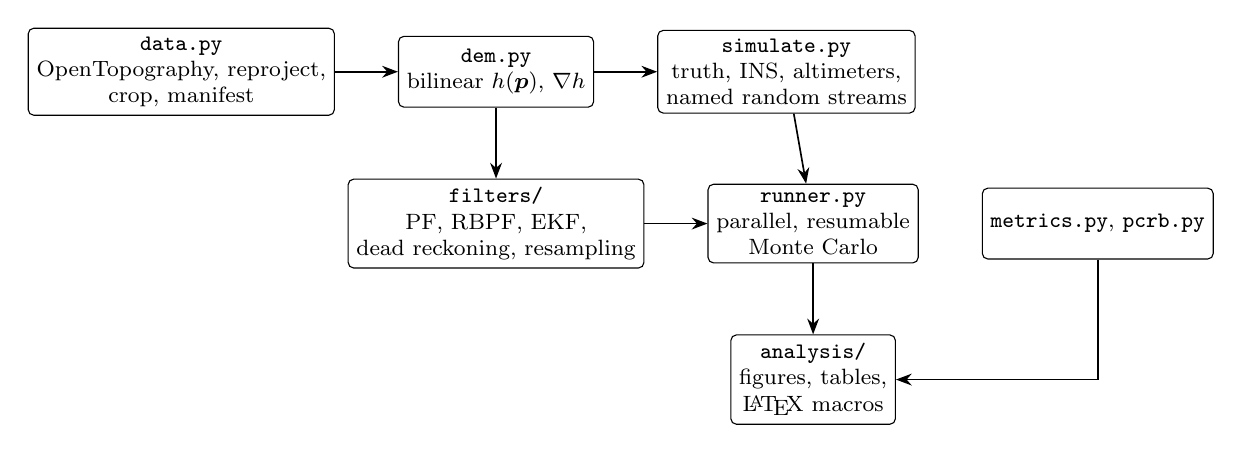
\begin{tikzpicture}[
      box/.style={draw, rounded corners=2pt, align=center, font=\footnotesize,
                  minimum height=9mm, inner sep=3pt},
      arr/.style={-{Stealth[length=2mm]}, semithick}]
    \node[box] (data) {\texttt{data.py}\\ OpenTopography, reproject,\\ crop, manifest};
    \node[box, right=8mm of data] (dem) {\texttt{dem.py}\\ bilinear $h(\pv)$, $\nabla h$};
    \node[box, right=8mm of dem] (sim) {\texttt{simulate.py}\\ truth, INS, altimeters,\\ named random streams};
    \node[box, below=9mm of dem] (filters) {\texttt{filters/}\\ PF, RBPF, EKF,\\ dead reckoning, resampling};
    \node[box, right=8mm of filters] (runner) {\texttt{runner.py}\\ parallel, resumable\\ Monte Carlo};
    \node[box, right=8mm of runner] (metrics) {\texttt{metrics.py}, \texttt{pcrb.py}};
    \node[box, below=9mm of runner] (analysis) {\texttt{analysis/}\\ figures, tables,\\ \LaTeX{} macros};
    \draw[arr] (data) -- (dem);
    \draw[arr] (dem) -- (sim);
    \draw[arr] (dem) -- (filters);
    \draw[arr] (sim) -- (runner);
    \draw[arr] (filters) -- (runner);
    \draw[arr] (runner) -- (analysis);
    \draw[arr] (metrics) |- (analysis);
  \end{tikzpicture}
  \caption{Package structure and data flow. Every estimator implements the same interface
    (\texttt{initialize}, \texttt{predict}, \texttt{update}, \texttt{estimate}), so the runner
    treats them identically. The report reads only the outputs of \texttt{analysis/}.}
  \label{fig:arch}
\end{figure}

\subsection{The particle filter}
\Cref{lst:predict,lst:update} are the predict and update steps of \cref{eq:sir}, copied from the
source by a script so that they cannot drift from the code. The particles are an $N\times4$
array; the prediction samples all $N$ motion-model draws at once, each particle integrating the
INS velocity corrected by its own bias. The update evaluates the DEM at all particle positions
with one vectorised bilinear lookup (\texttt{scipy.ndimage.map\_coordinates}), adds the
log-likelihood to the log-weights and renormalises with log-sum-exp. Particles that leave the DEM
get zero weight rather than reading a clamped edge height, which would compare the measurement with
fake flat terrain. The same pass computes the predicted measurement spread for the NIS of
\cref{sec:monitor} and the log evidence.

\lstinputlisting[caption={Particle filter prediction (\texttt{ParticleFilter.predict}).},
  label={lst:predict}]{../generated/code_pf_predict.py}

\lstinputlisting[caption={Particle filter measurement update (\texttt{ParticleFilter.update}).},
  label={lst:update}]{../generated/code_pf_update.py}

Systematic resampling (\cref{lst:systematic}) needs one uniform number: evenly spaced pointers
are located in the cumulative weights by a binary search. Pinning the last cumulative weight to
exactly 1 and searching with \texttt{side="right"} guarantee that a particle with zero weight is
never selected, even when a pointer lands on a boundary; a unit test checks this for all four
schemes.

\lstinputlisting[caption={Systematic resampling.},label={lst:systematic}]{../generated/code_systematic.py}

The Rao-Blackwellised filter stores its particles in the same $N\times4$ array, with the Kalman
bias means in the last two columns, so the parent class's weighting and resampling are reused
unchanged; only the prediction (\cref{lst:rbpf}) and the covariance differ.

\lstinputlisting[caption={RBPF prediction with the shared Riccati recursion
  (\texttt{RaoBlackwellizedPF.predict}).},label={lst:rbpf}]{../generated/code_rbpf_predict.py}

\subsection{Simulation}\label{sec:sim}
The simulator is the ``world'': it knows the true trajectory and is the only component that
reads the DEM at the true position. A flight starts at a uniformly random point with a random
heading, flies at 40\,m/s and weaves $\pm25^\circ$ with a 120\,s period. The whole flight stays
$3\times2000$\,m inside the map --- three times the largest initial uncertainty used --- so that
neither the truth nor the prior reaches the edge; flights that would are redrawn. The altitude is
constant: the highest terrain within 1\,km of the track plus 300\,m clearance. INS velocities
and altimeter readings follow \cref{sec:models}; optional radar outliers, a spatially correlated
map-error field and a constant offset are added for Experiment~4.

Each source of randomness has its own named random stream per Monte Carlo run (flight, INS,
altimeters, outliers, initial guess, map error, and one per filter family), and every draw has a
fixed size and is scaled afterwards. Run $i$ is therefore identical in every configuration: a
larger $\sigma_0$ scales the \emph{same} initial-error direction, a higher outlier rate adds
outliers \emph{at the same instants plus new ones}, and so on. Unit tests check these invariances.

\subsection{Experiments and reproducibility}
Experiments are YAML files: a grid of parameters, a list of regions and estimator variants and a
number of runs. One task simulates a flight once and runs every estimator on it; tasks run in
parallel worker processes that share the DEMs in memory, and each writes a compressed file of
time series and per-run metrics. An interrupted sweep resumes where it stopped, and each results
folder records the git commit, the data-manifest checksum, the resolved configurations and the
installed package versions. Figures, tables and every number quoted in this report are produced
by scripts from these saved results (\texttt{make figures}); the data are traced by SHA-256
checksums of the downloaded and processed rasters.

Runtimes come from a separate benchmark --- one process pinned to a performance core, one maths
thread --- because inside the parallel sweeps the workers share memory bandwidth and each runs
several times slower. \Cref{tab:runtime} lists the cost per filter step on the hill-country DEM:
the particle filter with $N = 5\,000$ needs \RtPfFiveZeroZeroZero{}\,ms per step, three orders
of magnitude faster than the 1\,Hz altimeter rate. The RBPF costs the same as the plain filter
at equal $N$ (\RtRbpfFiveZeroZeroZero{}\,ms): its bias update is cheap and it draws half as many
random numbers.

\begin{table}[t]
  \centering\small
  \caption{Runtime per filter step (median of \RtReps{} repetitions of a 300-step flight on the
    hill-country DEM, single process, one performance core of the machine in
    \cref{app:repro}).}\label{tab:runtime}
  % Generated by scripts — do not edit.
\begin{tabular}{lrrr}
\toprule
Estimator & $N$ & Median (ms/step) & IQR (ms/step) \\
\midrule
Dead reckoning & -- & 0.009 & 0.009--0.010 \\
EKF & -- & 0.046 & 0.046--0.047 \\
PF & 500 & 0.215 & 0.202--0.217 \\
PF & 1\,000 & 0.283 & 0.274--0.291 \\
PF & 2\,000 & 0.436 & 0.416--0.456 \\
PF & 5\,000 & 0.832 & 0.825--0.874 \\
PF & 10\,000 & 1.511 & 1.506--1.578 \\
PF & 20\,000 & 2.877 & 2.871--2.891 \\
PF & 50\,000 & 7.022 & 7.013--7.118 \\
RBPF & 500 & 0.242 & 0.230--0.247 \\
RBPF & 1\,000 & 0.296 & 0.292--0.310 \\
RBPF & 2\,000 & 0.434 & 0.433--0.447 \\
RBPF & 5\,000 & 0.832 & 0.829--0.872 \\
RBPF & 10\,000 & 1.483 & 1.477--1.485 \\
RBPF & 20\,000 & 2.797 & 2.790--2.799 \\
PF, Student-t & 5\,000 & 0.849 & 0.847--0.858 \\
PF + monitor & 5\,000 & 0.851 & 0.847--0.856 \\
\bottomrule
\end{tabular}

\end{table}

\subsection{Validation}\label{sec:validation}
Because the outputs of a particle filter are random, ``it converges on a test case'' is weak
evidence of correctness. The decisive test uses a terrain for which the exact answer is known: on
a tilted plane $h(\pv) = 0.05\,p_x + 0.03\,p_y + 200$ the measurement is linear and bilinear
interpolation is exact, so the EKF \emph{is} the Kalman filter and computes the exact posterior.
A correct particle filter must agree with it up to Monte Carlo error. Over \ValSeeds{} seeds and
all 300 steps, the particle filter's estimate never deviates from the Kalman estimate by more than
\ValPFPosMax{} Kalman standard deviations in position and \ValPFBiasMax{} in bias
(\cref{tab:validation}); the RBPF, with four times fewer particles, stays within
\ValRBPFPosMax{} and \ValRBPFBiasMax{} --- a first glimpse of the variance reduction that
Rao-Blackwellisation promises. On the same plane the PCRB recursion reproduces the Kalman
covariance to a relative difference of \ValPcrbRelDiff{}. Further unit tests cover the resampling
schemes (unbiased offspring counts, zero-weight particles never selected, systematic offspring
equal to $\lfloor N w\rfloor$ or $\lceil N w \rceil$), the likelihoods (normalised densities,
outlier robustness), the true-noise model of the bound (against the simulator's empirical noise),
the divergence monitor (silent while tracking, recovers from a forced false lock), the metrics
(Wilson intervals, $\chi^2$ bounds, McNemar test against closed forms) and the runner (common
random numbers across configurations, resumption).

\begin{table}[t]
  \centering\small
  \caption{Particle filters against the exact Kalman filter on planar terrain ($\sigma_0 =
    100$\,m, \ValSeeds{} seeds, worst case over the 300-step flight).}\label{tab:validation}
  % Generated by scripts — do not edit.
\begin{tabular}{lrrrr}
\toprule
Filter & $N$ & max $|\hat x - \hat x_{KF}|/\sigma_{KF}$, position & same, bias & trace ratio $P/P_{KF}$ (position) \\
\midrule
PF & 20\,000 & 0.11--0.57 & 0.06--0.18 & 0.62--1.20 \\
RBPF & 5\,000 & 0.06--0.19 & 0.05--0.13 & 0.85--1.36 \\
\bottomrule
\end{tabular}

\end{table}

\Cref{tab:params} in the appendix lists all parameters.

\section{Results}\label{sec:results}

Unless stated otherwise every experiment uses randomised 300\,s flights at 40\,m/s, the default
parameters of \cref{tab:params}, and common random numbers: within an experiment, run $i$ has the
same flight and noise for every filter and configuration. $M$ is the number of Monte Carlo runs
per configuration. Brackets give 95\,\% intervals (Wilson for rates, bootstrap for RMSE).

\subsection{Study regions}\label{sec:regions}
Three $0.36^\circ\times0.36^\circ$ boxes ($\approx40\times40$\,km) were chosen with a rule fixed
before the data were examined: on a 90\,m survey of the whole island, the roughest candidate box
around Nuwara Eliya, the flattest around Anuradhapura, and around Kandy the box whose roughness is
closest to the geometric mean of the two (\cref{fig:regions,tab:regions}). No box around Kandy is
nearly as smooth as that target, so the least rough one was selected: the ``Kandy'' region is
intermediate, but closer to the rugged end. The regions differ by two orders of magnitude in the
position information one altimeter sample carries (\cref{tab:terrain}): the Fisher information
density is \TerrHillFisherDensityPerMTwo{}, \TerrKandyFisherDensityPerMTwo{} and
\TerrPlainsFisherDensityPerMTwo{}\,$\times10^{-3}$\,m$^{-2}$ for the hill country, Kandy and the
plains. The synthetic terrain used during development has a 1\,km roughness similar to the hill
country (\TerrSyntheticRoughnessOnekmM{} vs.\ \TerrHillRoughnessOnekmM{}\,m) but less than half of
its information density: smooth Gaussian hills lack the slope texture of real terrain at the
scale of a few cells --- a difference that turns out to matter for the EKF.

\begin{figure}[t]
  \centering
  \begin{subfigure}[b]{0.34\textwidth}\centering
    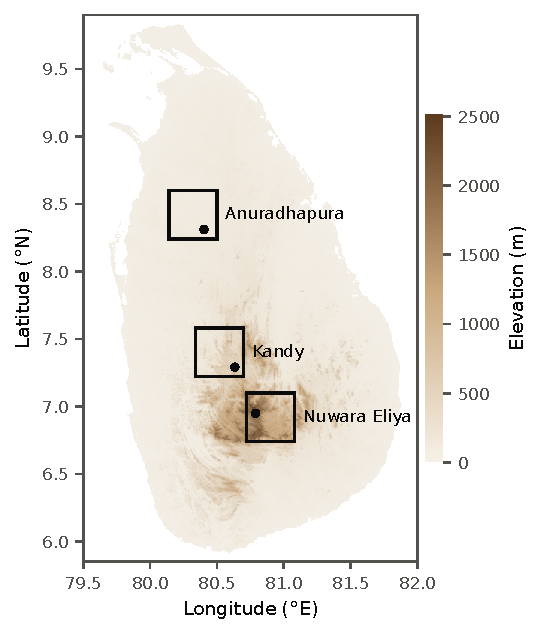
\includegraphics[width=\textwidth]{region_map.pdf}\caption{Sri Lanka (COP90 survey).}
  \end{subfigure}\hfill
  \begin{subfigure}[b]{0.64\textwidth}\centering
    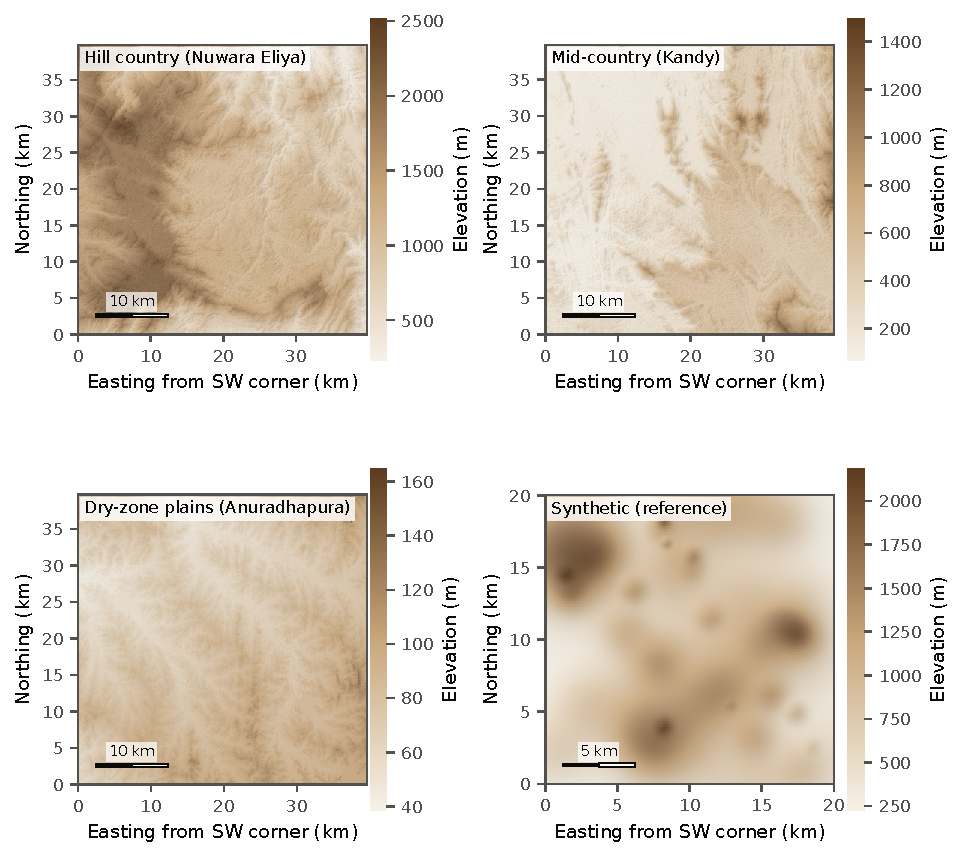
\includegraphics[width=\textwidth]{terrain_overview.pdf}\caption{The three regions and the synthetic reference.}
  \end{subfigure}
  \caption{Study regions. Boxes in (a) were selected by the pre-registered roughness rule;
    (b) shows the 30\,m Copernicus GLO-30 elevation (colour) with hillshading. Note the different
    elevation scales: the plains span only 127\,m.}\label{fig:regions}
\end{figure}

\begin{table}[t]
  \centering\small
  \caption{Study regions as requested from OpenTopography and the processed UTM grids.}\label{tab:regions}
  % Generated by scripts — do not edit.
\begin{tabular}{lrrrr}
\toprule
Region & Latitude ($^\circ$N) & Longitude ($^\circ$E) & Size (km) & Grid (30 m cells) \\
\midrule
Hill country (Nuwara Eliya) & 6.74--7.10 & 80.72--81.08 & 39.8 $\times$ 39.8 & 1327\,$\times$\,1325 \\
Mid-country (Kandy) & 7.22--7.58 & 80.34--80.70 & 39.7 $\times$ 39.8 & 1326\,$\times$\,1323 \\
Dry-zone plains (Anuradhapura) & 8.24--8.60 & 80.14--80.50 & 39.6 $\times$ 39.8 & 1325\,$\times$\,1319 \\
\bottomrule
\end{tabular}

\end{table}

\begin{table}[t]
  \centering\small
  \caption{Terrain statistics (definitions in \cref{sec:data}).}\label{tab:terrain}
  % Generated by scripts — do not edit.
\begin{tabular}{lrrrr}
\toprule
Statistic & Hill country & Kandy & Dry-zone plains & Synthetic \\
\midrule
Min.\ elevation (m) & 224 & 64 & 38 & 221 \\
Max.\ elevation (m) & 2\,521 & 1\,499 & 165 & 2\,190 \\
Elevation range (m) & 2\,297 & 1\,436 & 127 & 1\,970 \\
Elevation std (m) & 450 & 215 & 16 & 381 \\
Mean slope (\%) & 35.0 & 24.2 & 3.1 & 22.6 \\
Slope std (\%) & 21.0 & 17.6 & 2.4 & 14.7 \\
Roughness, 1 km window (m) & 64.5 & 37.7 & 3.5 & 62.7 \\
Fisher density ($10^{-3}$\,m$^{-2}$) & 13.49 & 7.38 & 0.16 & 5.63 \\
Grid (cells) & 1327\,$\times$\,1325 & 1326\,$\times$\,1323 & 1325\,$\times$\,1319 & 667\,$\times$\,667 \\
\bottomrule
\end{tabular}

\end{table}

\subsection{E1 --- When does linearisation fail?}\label{sec:e1}
\emph{Setup:} dead reckoning, EKF and particle filters with 5\,000 and 20\,000 particles on
identical flights; $\sigma_0 \in \{100, 250, 500, 1000, 1500, 2000\}$\,m on all three regions;
$M = \EOneRuns$ per cell (5\,400 flights in total).

\begin{figure}[t]
  \centering
  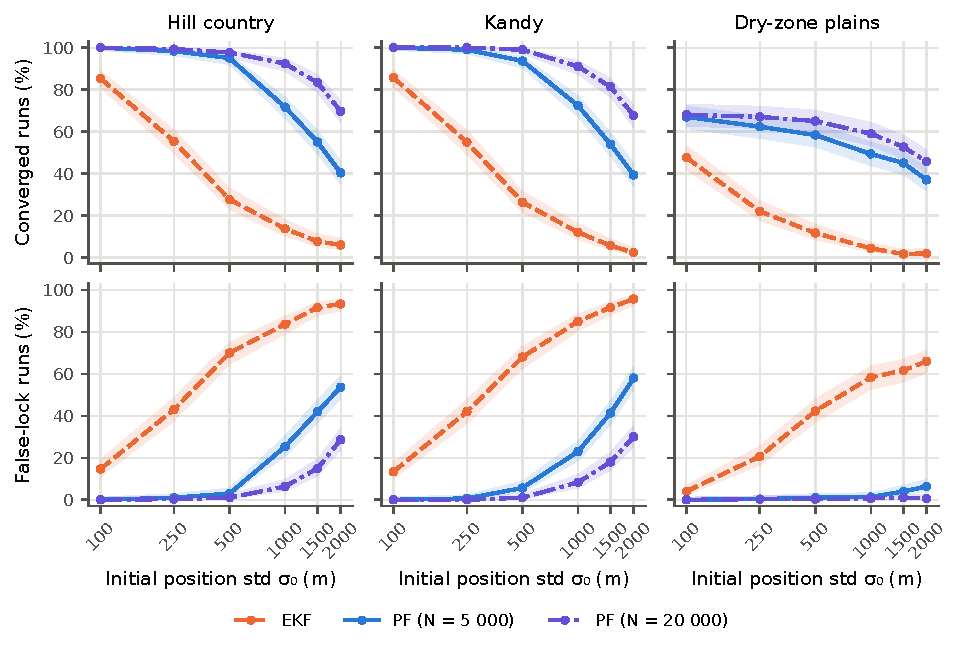
\includegraphics[width=\textwidth]{e1_rates.pdf}
  \caption{E1: share of converged (top) and falsely locked (bottom) runs against the initial
    position uncertainty, $M = \EOneRuns$ per point, Wilson 95\,\% bands. Dead reckoning never
    converges and is omitted.}\label{fig:e1rates}
\end{figure}

\begin{figure}[t]
  \centering
  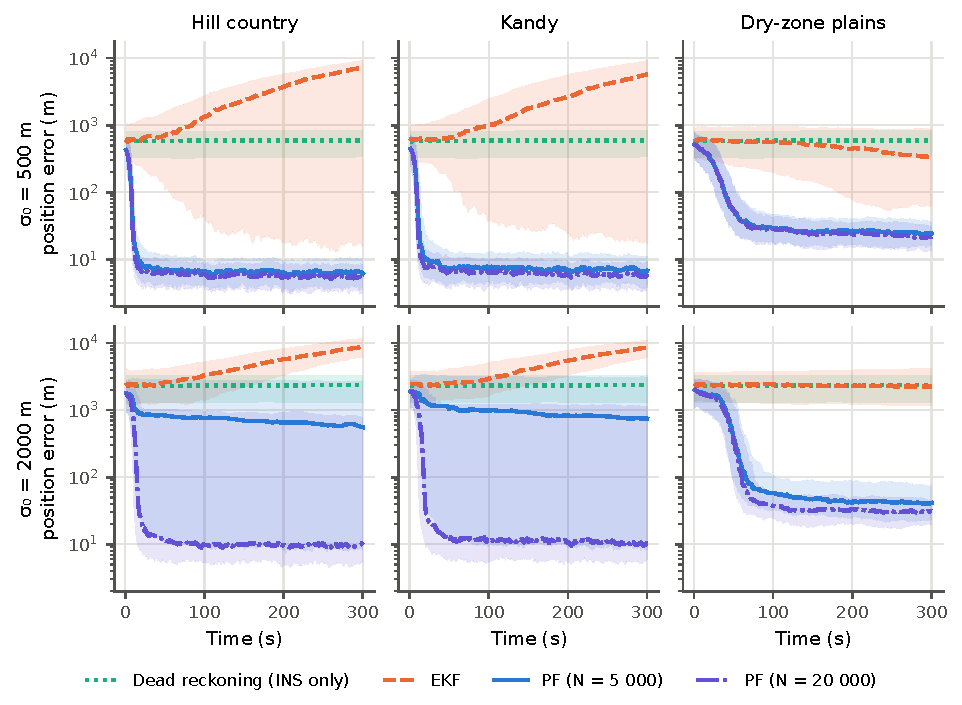
\includegraphics[width=\textwidth]{e1_error_vs_time.pdf}
  \caption{E1: median position error over time (bands: interquartile range over the
    $M = \EOneRuns$ runs) for $\sigma_0 = 500$\,m (top) and 2\,000\,m (bottom). Log scale.}\label{fig:e1time}
\end{figure}

\Cref{fig:e1rates} answers the question directly, and the answer depends strongly on the
terrain. On the hill country the EKF fails even when the initial error is small: at
$\sigma_0 = 100$\,m it converges in only \EOneHillSOneZeroZeroEkfConv\,\% of the runs and
falsely locks in \EOneHillSOneZeroZeroEkfFl\,\%; at 500\,m it converges in
\EOneHillSFiveZeroZeroEkfConv\,\% and is confidently wrong in \EOneHillSFiveZeroZeroEkfFl\,\%. The
particle filters converge in \EOneHillSFiveZeroZeroPfFiveZeroZeroZeroConv\,\% ($N=5\,000$) and
\EOneHillSFiveZeroZeroPfTwoZeroZeroZeroZeroConv\,\% ($N=20\,000$) of the same runs. Paired over the
runs, the PF converges significantly more often than the EKF in every one of the 18 cells
(McNemar, all $p < 10^{-10}$; \cref{tab:e1tests} in the appendix). This is a much earlier failure
than on the smooth synthetic terrain, where the EKF had held up to $\sigma_0 = 1$\,km during
development: the real DEM's slope changes within a few cells, so the one-cell Jacobian is already
wrong when the error is a few tens of metres. The Kandy region behaves almost identically.

\Cref{fig:e1time} shows how the EKF fails. Its median error \emph{grows} during the flight and
ends well above the dead-reckoning error on both hilly regions: corrections computed from the
wrong slope also corrupt the bias estimate, so the EKF drifts faster than the uncorrected INS.
A linearised terrain filter is worse than no terrain aiding at all once its linearisation is
invalid.

The particle filter's limit is different. Its error drops within 10--20\,s to a few metres, and
it degrades gracefully with $\sigma_0$: at 2\,km the filter with 20\,000 particles still converges in
\EOneHillSTwoZeroZeroZeroPfTwoZeroZeroZeroZeroConv\,\% of the runs, the one with 5\,000 in
\EOneHillSTwoZeroZeroZeroPfFiveZeroZeroZeroConv\,\%. Its failures are almost all false locks
(\EOneHillSTwoZeroZeroZeroPfFiveZeroZeroZeroFl\,\% and
\EOneHillSTwoZeroZeroZeroPfTwoZeroZeroZeroZeroFl\,\%): with a wide prior, few particles start
close enough to the truth, and the cloud collapses onto another patch whose profile matches.
More particles help significantly from $\sigma_0 \ge 500$\,m on every region.

The flat plains tell the opposite story about failure. No filter converges reliably: even at
$\sigma_0 = 100$\,m the 20\,000-particle PF converges in only
\EOnePlainsSOneZeroZeroPfTwoZeroZeroZeroZeroConv\,\% of the runs, and in
\EOnePlainsSTwoZeroZeroZeroPfTwoZeroZeroZeroZeroConv\,\% at 2\,km. Yet it almost never locks
falsely (\EOnePlainsSTwoZeroZeroZeroPfTwoZeroZeroZeroZeroFl\,\% at 2\,km): it knows that it does
not know. Its covariance stays wide, and its median error still falls from 500\,m to about 25\,m
within the first 100\,s, because even 3\,m of roughness is not zero information; most of its
``non-converged'' runs end just above the 50\,m threshold rather than lost (\cref{sec:e2}). The
EKF on the plains, by contrast, is falsely locked in \EOnePlainsSFiveZeroZeroEkfFl\,\% of the runs
at $\sigma_0 = 500$\,m. In the tracking phase
of converged runs the PF's RMSE is \EOneHillSFiveZeroZeroPfTwoZeroZeroZeroZeroTrack\,m (hill
country), \EOneKandySFiveZeroZeroPfTwoZeroZeroZeroZeroTrack\,m (Kandy) and
\EOnePlainsSFiveZeroZeroPfTwoZeroZeroZeroZeroTrack\,m (plains) at $\sigma_0 = 500$\,m
(\cref{tab:e1track} in the appendix).

The corridor rule for the altitude puts the UAV up to \EOneRadarHillMax\,m above the terrain on
the hill country (median of the per-flight maximum \EOneRadarHillMedian\,m); a range-independent
3\,m radar noise is optimistic at such ranges, which is a limitation of the sensor model
(\cref{sec:limitations}).

\subsection{E2 --- Terrain informativeness}\label{sec:e2}
\emph{Setup:} EKF and PF ($N = 5\,000$), $\sigma_0 = 500$\,m, $M = \ETwoRuns$ random flights
per region. For every flight the terrain under the true track is characterised by its mean 1\,km
roughness and by the terrain information $\sum_k |\nabla h(\pv_k)|^2/\sigma_z^2$, split into
along- and cross-track components.

\begin{figure}[t]
  \centering
  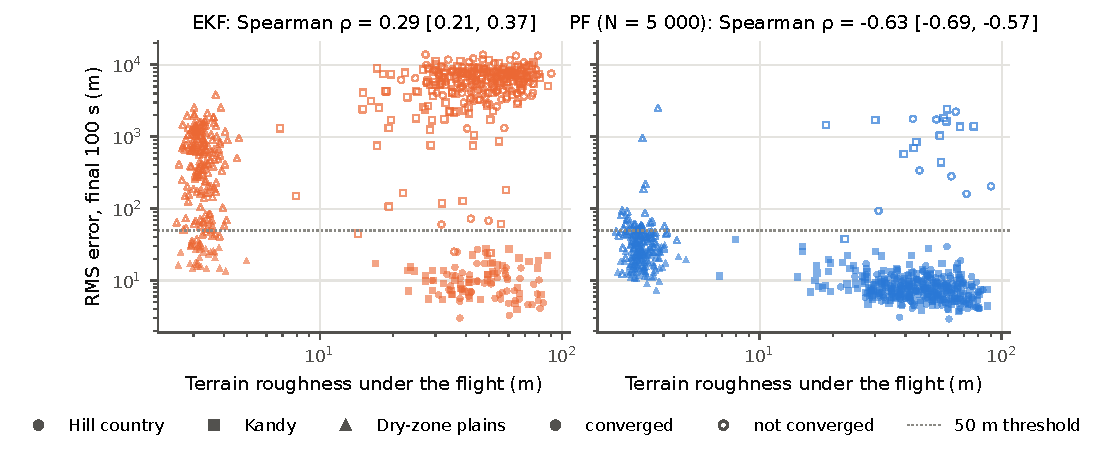
\includegraphics[width=\textwidth]{e2_scatter.pdf}
  \caption{E2: RMS error over the final 100\,s of each flight against the roughness of the
    terrain under that flight ($M = \ETwoRuns$ per region, $\sigma_0 = 500$\,m). Spearman rank
    correlation with bootstrap 95\,\% CI over all flights.}\label{fig:e2scatter}
\end{figure}

\Cref{fig:e2scatter} relates each flight's final error to the terrain it crossed. For the particle
filter, rougher terrain means smaller error (Spearman $\rho = \ETwoRhoPfFiveZeroZeroZero$
[$\ETwoRhoPfFiveZeroZeroZeroLo$, $\ETwoRhoPfFiveZeroZeroZeroHi$]). For the EKF the correlation has
the \emph{opposite} sign ($\rho = \ETwoRhoEkf$ [$\ETwoRhoEkfLo$, $\ETwoRhoEkfHi$]): the same texture that informs
the particle filter breaks the EKF's linearisation, so its failures concentrate on the most
informative terrain. Within a single region the correlations are weak (PF $\rho$ between
\ETwoPlainsPfFiveZeroZeroZeroRho{} and \ETwoKandyPfFiveZeroZeroZeroRho), i.e.\ most of the effect
is between terrain types rather than between flights over the same type. Binned by the terrain
information collected along the flight (\cref{fig:e2binned}), the PF's convergence rate rises
from about one half on the least informative flights to over 90\,\% on the hills.

\begin{figure}[t]
  \centering
  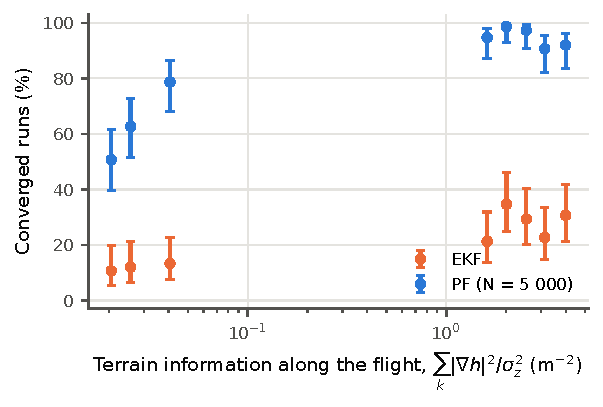
\includegraphics[width=0.62\textwidth]{e2_binned.pdf}
  \caption{E2: convergence against the terrain information along the flight (eight equal-count
    bins pooled over the three regions; Wilson 95\,\% intervals). No flight falls between the
    plains and the hills, hence the gap.}\label{fig:e2binned}
\end{figure}

Decomposing the tracking error into along- and cross-track components (\cref{tab:e2}) shows no
systematic anisotropy: the PF's along/cross RMS is \ETwoHillPfFiveZeroZeroZeroAlong{}/%
\ETwoHillPfFiveZeroZeroZeroCross\,m on the hill country, \ETwoKandyPfFiveZeroZeroZeroAlong/%
\ETwoKandyPfFiveZeroZeroZeroCross\,m around Kandy and \ETwoPlainsPfFiveZeroZeroZeroAlong/%
\ETwoPlainsPfFiveZeroZeroZeroCross\,m on the plains, and the along- and cross-track terrain
information is balanced on average (ratio $\approx 1$). The expected elongation of the error along
ridges and valleys does not appear in these averages: the 25$^\circ$ heading weave and the varied
ridge directions inside 40\,km boxes mix the two directions. The hypothesis is therefore not
supported at the ensemble level; it may still hold for individual straight flights along a valley,
which this design does not isolate.

\begin{table}[t]
  \centering\small
  \caption{E2 per region ($\sigma_0 = 500$\,m, $M = \ETwoRuns$): convergence, median roughness
    under the flights, tracking RMS along and across the track (converged runs), median ratio of
    along- to cross-track terrain information, and the within-region Spearman correlation between
    roughness and final error.}\label{tab:e2}
  % Generated by scripts — do not edit.
\begin{tabular}{llrrrrrr}
\toprule
Region & Filter & Conv.\ (\%) [95\% CI] & Rough.\ (m) & Along RMS (m) & Cross RMS (m) & $I_\parallel/I_\perp$ & $\rho_S$ \\
\midrule
Hill country & EKF & 26 [21, 33] & 48.3 & 7.6 & 8.0 & 1.01 & -0.07 \\
Hill country & PF (N = 5 000) & 96 [92, 98] & 48.3 & 6.0 & 6.0 & 1.01 & -0.16 \\
Kandy & EKF & 26 [21, 33] & 41.6 & 9.5 & 9.5 & 0.97 & 0.16 \\
Kandy & PF (N = 5 000) & 94 [89, 96] & 41.6 & 7.4 & 7.5 & 0.97 & -0.26 \\
Dry-zone plains & EKF & 12 [9, 18] & 3.2 & 14.7 & 17.5 & 1.03 & -0.07 \\
Dry-zone plains & PF (N = 5 000) & 60 [53, 67] & 3.2 & 14.7 & 15.4 & 1.03 & -0.05 \\
\bottomrule
\end{tabular}

\end{table}

\subsection{E3 --- Particle-filter design}\label{sec:e3}
\emph{Setup:} hill country, $\sigma_0 = 1$\,km, $M = \EThreeRuns$; one design parameter varied at
a time from the defaults (systematic resampling, $\tau = 0.5$, $K = 0$).

\begin{figure}[t]
  \centering
  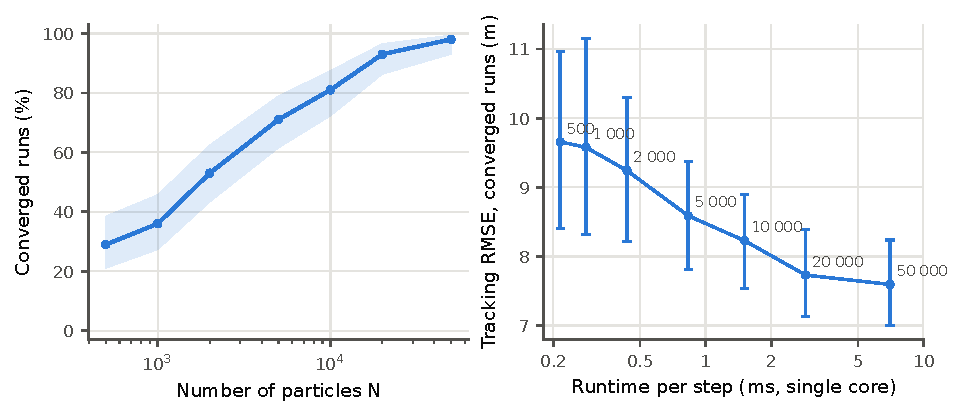
\includegraphics[width=\textwidth]{e3_particles.pdf}
  \caption{E3: convergence against the number of particles (left) and tracking RMSE of converged
    runs against the runtime per step from the single-core benchmark (right, labelled with $N$);
    $M = \EThreeRuns$, hill country, $\sigma_0 = 1$\,km.}\label{fig:e3n}
\end{figure}

\paragraph{Number of particles.} Convergence rises from \EThreeNFiveHundredConv\,\% with 500
particles to \EThreeNFiveKConv\,\% with 5\,000 and \EThreeNFiftyKConv\,\% with 50\,000
(\cref{fig:e3n}), while the tracking RMSE improves only from \EThreeNFiveHundredTrack{} to
\EThreeNFiftyKTrack\,m. Particles buy \emph{robustness of acquisition} much more than tracking accuracy:
once locked on, 500 particles track within about 2\,m of fifty thousand. The cost is
linear in $N$; even $N = 50\,000$ needs only \EThreeNFiftyKMs\,ms per step on one core, two
orders of magnitude inside the real-time budget of a 1\,Hz altimeter.

\paragraph{Resampling.} The four schemes do not differ significantly in convergence (McNemar
$p \ge 0.15$ against systematic at both $N$; \cref{tab:e3tests}) or tracking RMSE (overlapping
intervals, \cref{fig:e3design}). The schemes do differ in what they are designed to differ in:
measured directly, the variance of the offspring counts (\cref{tab:e3var}) is
\EThreeVarMultinomialFiveK{} for multinomial (theory 1.00), \EThreeVarResidualFiveK{} for residual
(theory 0.44), \EThreeVarStratifiedFiveK{} for stratified and \EThreeVarSystematicFiveK{} for
systematic resampling --- the last equal to the minimum possible for any unbiased scheme
(\EThreeVarFloorFiveK, attained when every count is $\lfloor N w\rfloor$ or $\lceil N w\rceil$).
This matches Hol, Schön and Gustafsson~\cite{hol2006}, who found stratified and residual
resampling to have lower variance than multinomial, recommended systematic resampling for its
quality and cost, and found the effect on the estimates ``not significant''; here too the lower
resampling noise is real but small compared with the other sources of error, and systematic
resampling is also the cheapest (\cref{tab:runtime}).

\paragraph{ESS threshold.} Resampling when $\Neff$ falls below $0.1N$ to $1.0N$ (every step)
changes the number of resampling steps per flight from \EThreeEssZeroPointOneResamples{} to
\EThreeEssOnePointZeroResamples{}, but not the convergence (\EThreeEssZeroPointOneConv--%
\EThreeEssOnePointZeroConv\,\%, all $p \ge 0.5$) or the tracking error.

\paragraph{Roughening.} Roughening has by far the largest effect of the design choices
(\cref{fig:e3design}, right). A small jitter, $K = 0.05$, raises convergence from
\EThreeRoughZeroPointZeroZeroConv\,\% to \EThreeRoughZeroPointZeroFiveConv\,\% (McNemar: 24 runs
gained, 1 lost, $p < 10^{-4}$) and also lowers the tracking RMSE (\EThreeRoughZeroPointZeroFiveTrack{}
vs.\ \EThreeRoughZeroPointZeroZeroTrack\,m); $K = 0.1$ gives \EThreeRoughZeroPointOneZeroConv\,\%
and $K = 0.2$ falls back to \EThreeRoughZeroPointTwoZeroConv\,\%. With $K = 0.05$, 5\,000 particles
match 20\,000 particles without roughening at a quarter of the cost. Because the jitter is
proportional to the spread of the cloud ($\sigma_j = K E_j N^{-1/4}$), roughening acts as an
\emph{adaptive} process-noise inflation: tens of metres while the cloud is still wide, which keeps
hypotheses near the truth alive between resamplings, and negligible once the cloud has collapsed.
Too much of it blurs the information the measurements provide.

\begin{figure}[t]
  \centering
  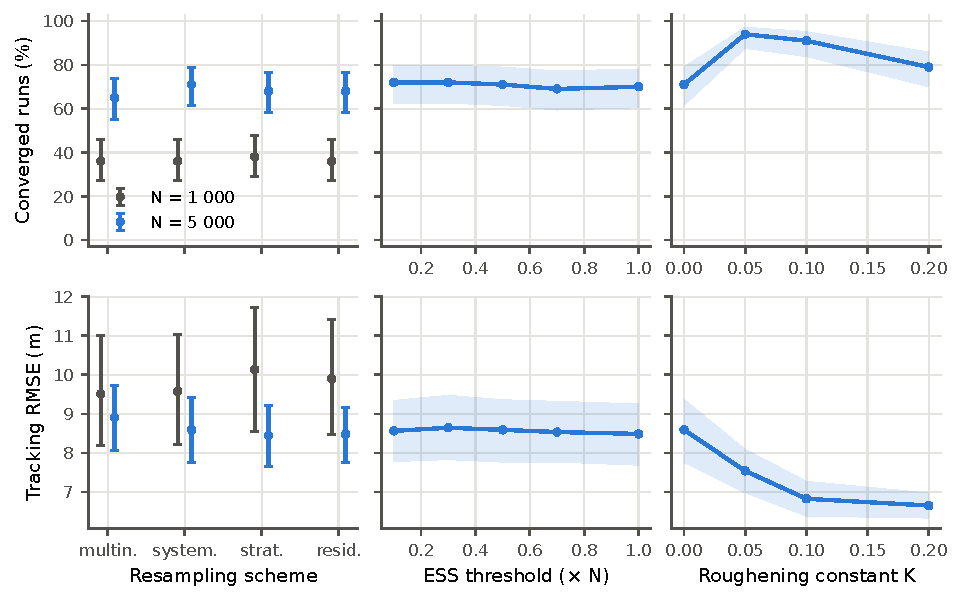
\includegraphics[width=\textwidth]{e3_design.pdf}
  \caption{E3: convergence (top) and tracking RMSE (bottom) for the resampling scheme (left,
    $N = 1\,000$ grey and 5\,000 blue), the ESS threshold (middle) and the roughening constant
    (right); $N = 5\,000$ unless stated, $M = \EThreeRuns$, 95\,\% intervals.}\label{fig:e3design}
\end{figure}

\begin{table}[t]
  \centering\small
  \caption{E3: measured variance of the offspring counts, mean over particles
    ($N_{\mathrm{eff}} \approx 0.4N$, 400 resamplings of one weight vector), with the closed forms
    for multinomial and residual resampling and the floor/ceil lower bound.}\label{tab:e3var}
  % Generated by scripts — do not edit.
\begin{tabular}{rrrrrrrr}
\toprule
$N$ & Multinomial & Systematic & Stratified & Residual & Multin.\ theory & Resid.\ theory & floor/ceil bound \\
\midrule
1\,000 & 1.001 & 0.180 & 0.269 & 0.438 & 0.997 & 0.438 & 0.179 \\
5\,000 & 1.000 & 0.179 & 0.277 & 0.442 & 1.000 & 0.441 & 0.179 \\
\bottomrule
\end{tabular}

\end{table}

\subsection{E4 --- Robustness to model mismatch}\label{sec:e4}
\emph{Setup:} hill country and Kandy (where a nominal filter converges, so there is something to
lose), $\sigma_0 = 500$\,m, $M = \EFourRuns$ per cell; the simulated world violates one model
assumption at a time while the filters keep their nominal models unless stated.

\begin{figure}[t]
  \centering
  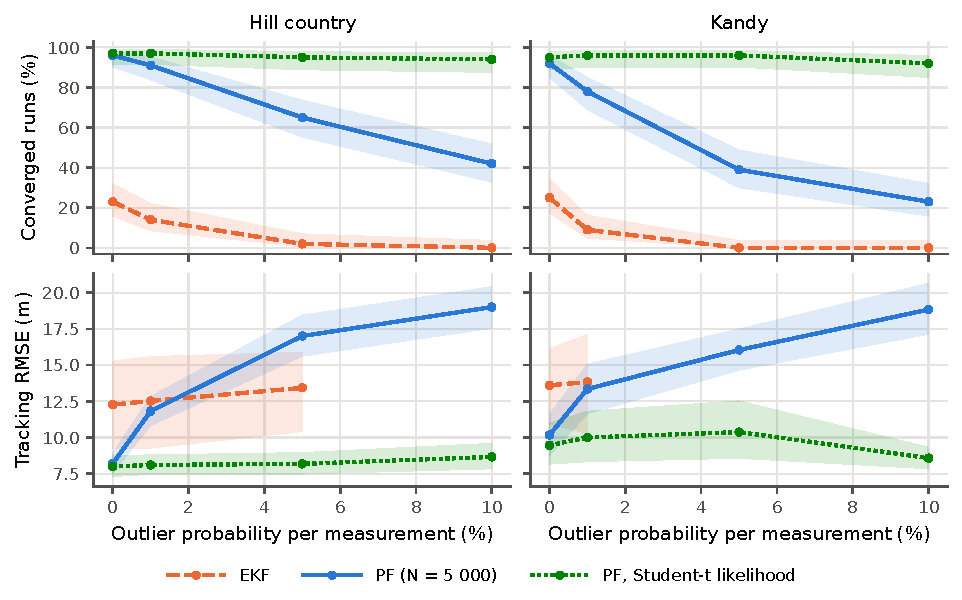
\includegraphics[width=\textwidth]{e4_outliers.pdf}
  \caption{E4: radar-altimeter outliers ($\mathcal{N}(0, 100^2)$\,m with the given probability per
    measurement). Gaussian vs.\ Student-$t$ ($\nu = 4$) likelihood; $M = \EFourRuns$, 95\,\%
    intervals.}\label{fig:e4outliers}
\end{figure}

\paragraph{Altimeter outliers.} With the Gaussian likelihood the particle filter's convergence on
the hill country falls from \EFourOutliersHillZeroPfFiveZeroZeroZeroConv\,\% without outliers to
\EFourOutliersHillOnePfFiveZeroZeroZeroConv\,\%, \EFourOutliersHillFivePfFiveZeroZeroZeroConv\,\%
and \EFourOutliersHillOneZeroPfFiveZeroZeroZeroConv\,\% when 1, 5 and 10\,\% of the radar samples
are gross errors (\cref{fig:e4outliers}): one outlier can wipe out the particles at the truth
(\cref{sec:studentt}). The Student-$t$ likelihood removes the problem: \EFourOutliersHillZeroPfStudentTConv,
\EFourOutliersHillOnePfStudentTConv, \EFourOutliersHillFivePfStudentTConv{} and
\EFourOutliersHillOneZeroPfStudentTConv\,\% for the same runs, with an unchanged tracking error,
and it costs nothing when there are no outliers. The EKF, already fragile, does not converge at
all once outliers are frequent.

\begin{figure}[t]
  \centering
  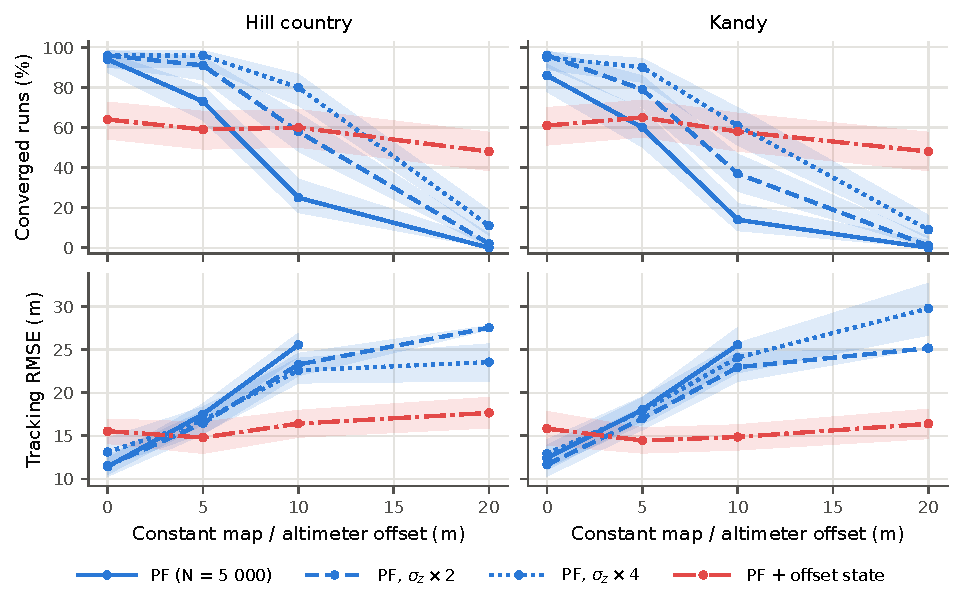
\includegraphics[width=\textwidth]{e4_map_error.pdf}
  \caption{E4: map error --- a spatially correlated field (std 2.4\,m, correlation length 1\,km,
    both assumptions derived from the handbook accuracy) plus a constant offset between the
    measured and the mapped surface. Remedies: measurement std inflated $\times2$ and $\times4$,
    and an extra state for the offset. $M = \EFourRuns$. The EKF is in \cref{tab:e4} only.}
  \label{fig:e4map}
\end{figure}

\paragraph{Map error.} A random map-error field of the size the Copernicus handbook implies is
harmless (\EFourMapErrorHillZeroPfFiveZeroZeroZeroConv\,\% convergence; \cref{fig:e4map}). A
\emph{constant} offset between the measured and the mapped height --- a barometric bias, or a radar
that sees the ground under a canopy the surface model includes --- is not: the nominal filter
converges in \EFourMapErrorHillFivePfFiveZeroZeroZeroConv\,\% of the runs at 5\,m,
\EFourMapErrorHillOneZeroPfFiveZeroZeroZeroConv\,\% at 10\,m and
\EFourMapErrorHillTwoZeroPfFiveZeroZeroZeroConv\,\% at 20\,m, because a profile shifted in height
matches the map best at the wrong place. Inflating $\sigma_z$ fourfold tolerates the offset up
to 10\,m (\EFourMapErrorHillOneZeroPfSzXFourConv\,\%) but not 20\,m
(\EFourMapErrorHillTwoZeroPfSzXFourConv\,\%). Estimating the offset as a fifth state is the only
remedy that still works at 20\,m (\EFourMapErrorHillTwoZeroPfHbiasConv\,\%), and it recovers the
offset itself (mean estimate \EFourHbHillOTwoZeroMean\,m for a true 20\,m; \cref{tab:e4hb}). It
pays for this when there is no offset: \EFourMapErrorHillZeroPfHbiasConv\,\% instead of
\EFourMapErrorHillZeroPfFiveZeroZeroZeroConv\,\%, because with an unknown offset a terrain
profile matches at more places, and the same 5\,000 particles now have to cover five dimensions.
This is a genuine trade-off, not a free improvement.

\paragraph{INS grade.} With an initial bias std of 0.1, 0.3 and 1.0\,m/s the particle filter
converges in \EFourInsGradeHillZeroPointOnePfFiveZeroZeroZeroConv,
\EFourInsGradeHillZeroPointThreePfFiveZeroZeroZeroConv{} and
\EFourInsGradeHillOnePfFiveZeroZeroZeroConv\,\% of the runs (EKF:
\EFourInsGradeHillZeroPointOneEkfConv, \EFourInsGradeHillZeroPointThreeEkfConv,
\EFourInsGradeHillOneEkfConv\,\%) and its tracking error grows with the bias
(\cref{fig:e4ins}): a poor INS makes the terrain do more of the work.

\begin{figure}[t]
  \centering
  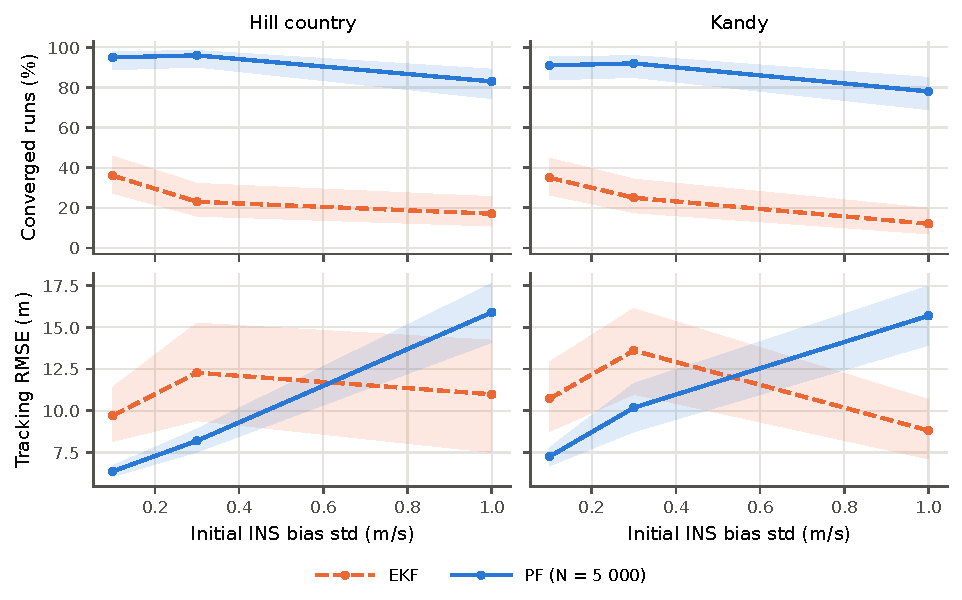
\includegraphics[width=\textwidth]{e4_ins_grade.pdf}
  \caption{E4: INS grade (initial velocity-bias std per axis); $M = \EFourRuns$. Dead reckoning
    never converges and is omitted.}\label{fig:e4ins}
\end{figure}

\begin{table}[t]
  \centering\small
  \caption{E4: offset estimated by the offset-state PF (mean over the final 100\,s, converged
    runs).}\label{tab:e4hb}
  % Generated by scripts — do not edit.
\begin{tabular}{lrrrr}
\toprule
Region & True offset (m) & Converged runs & Mean estimate (m) & Std of error (m) \\
\midrule
Hill country & 0 & 64 & -0.7 & 4.0 \\
Hill country & 10 & 60 & 10.2 & 4.3 \\
Hill country & 20 & 48 & 18.3 & 4.3 \\
Hill country & 5 & 59 & 5.1 & 3.3 \\
Kandy & 0 & 61 & 0.9 & 4.2 \\
Kandy & 10 & 58 & 10.4 & 4.1 \\
Kandy & 20 & 48 & 19.4 & 4.6 \\
Kandy & 5 & 65 & 4.8 & 3.7 \\
\bottomrule
\end{tabular}

\end{table}

\subsection{E5 --- Consistency and the theoretical bound}\label{sec:e5}
\emph{Setup:} the ensemble analysis reuses the E1 runs ($M = \EOneRuns$ per cell); the
per-flight analysis flies five fixed flight plans per region, each $M = 100$ times with fresh
sensor noise and initial error ($\sigma_0 = 500$\,m). The bounds use the true noise of the
simulation (\cref{sec:pcrb}).

\begin{figure}[t]
  \centering
  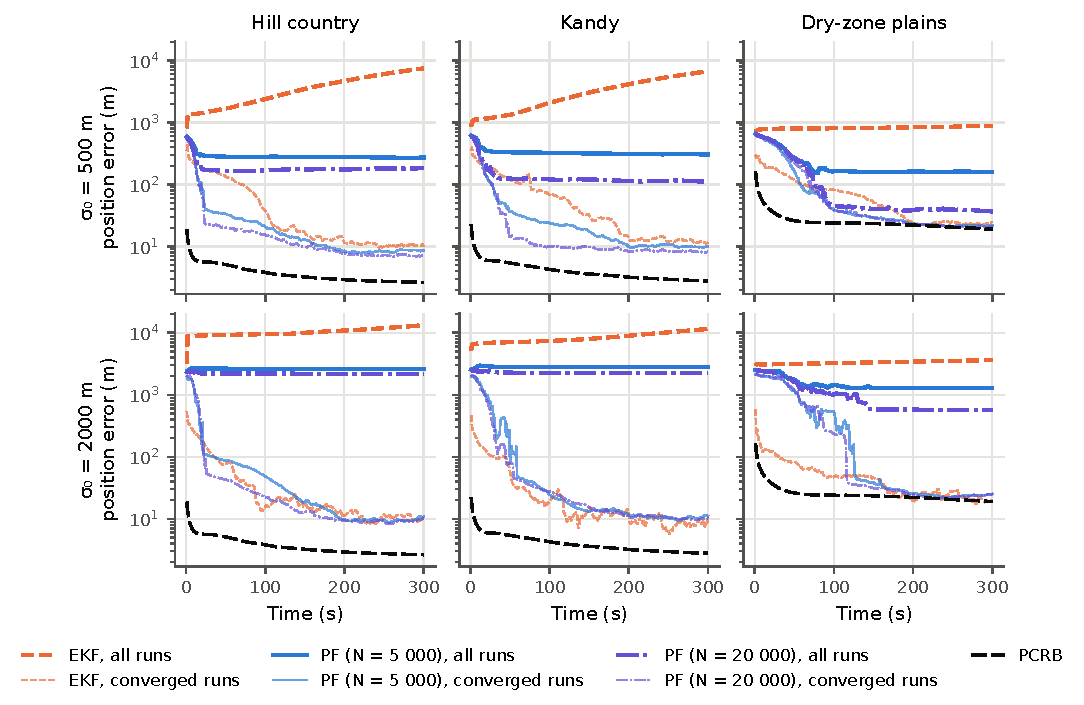
\includegraphics[width=\textwidth]{e5_bound.pdf}
  \caption{E5: RMSE over all runs (thick) and over converged runs (thin) against the ensemble
    PCRB (black), from the E1 runs ($M = \EOneRuns$).}\label{fig:e5bound}
\end{figure}

\paragraph{The bound and ambiguity.} The posterior Cramér--Rao bound is never violated: over all
regions, $\sigma_0$ and filters the all-run RMSE is at least 1.1 times the bound at every time step
(\cref{tab:e5cons}), a useful end-to-end check of the simulation, the filters and the bound. How
far above the bound the filters are depends on ambiguity (\cref{fig:e5bound}). The bound drops to
a few metres within seconds on the hilly regions (\EFiveHillSFiveZeroZeroBound\,m in the tracking
window on the hill country), because it only uses the slope at the true position: it describes a
filter that already knows which hill it is over. With $\sigma_0 = 100$\,m, where false locks do not
occur, the 20\,000-particle PF's all-run RMSE in the tracking window is
\EFiveHillSOneZeroZeroPfTwoZeroZeroZeroZeroBoundRatioAll{} times the bound on the hill country and
\EFivePlainsSOneZeroZeroPfTwoZeroZeroZeroZeroBoundRatioAll{} times on the plains; at $\sigma_0 =
500$\,m the few false locks alone raise the hill-country ratio to
\EFiveHillSFiveZeroZeroPfTwoZeroZeroZeroZeroBoundRatioAll. The gap between the thick and thin
curves in \cref{fig:e5bound} is the price of ambiguity, which no bound based on local slopes can
capture.

\begin{figure}[t]
  \centering
  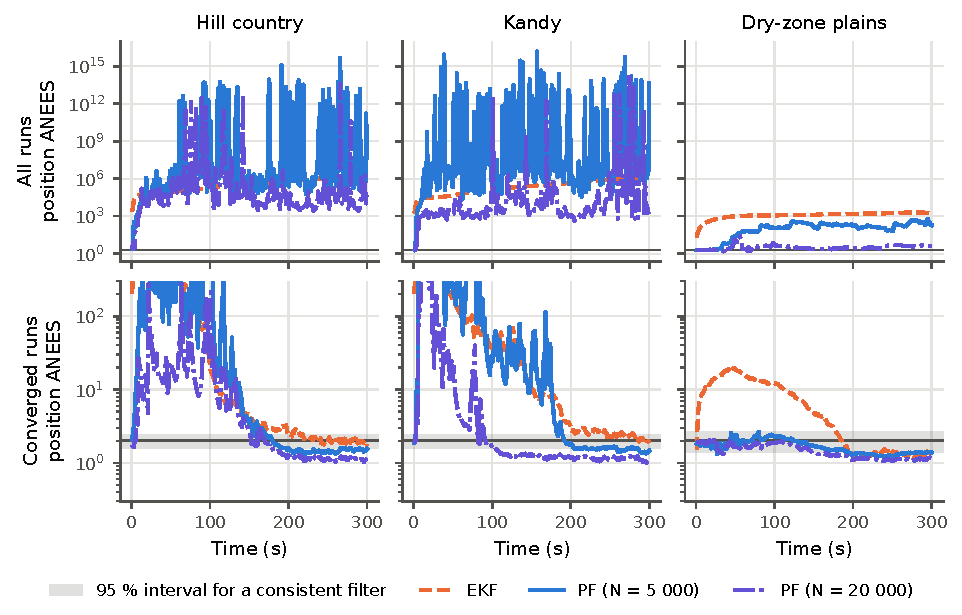
\includegraphics[width=\textwidth]{e5_anees.pdf}
  \caption{E5: position ANEES over all runs (top) and over converged runs (bottom) at
    $\sigma_0 = \EFiveAneesSigma$\,m, with the 95\,\% interval for a consistent filter (grey band;
    $M = \EOneRuns$). Log scale.}\label{fig:e5anees}
\end{figure}

\paragraph{Consistency.} Over all runs the ANEES is meaningless --- up to $10^{15}$ --- because a
falsely locked cloud is tight and far from the truth (\cref{fig:e5anees}, top). In the tracking
window of converged runs the PF is consistent to slightly conservative: ANEES
\EFiveHillSOneZeroZeroPfTwoZeroZeroZeroZeroAneesConv{} at $\sigma_0 = 100$\,m and
\EFiveHillSFiveZeroZeroPfTwoZeroZeroZeroZeroAneesConv{} at 500\,m on the hill country, against a
95\,\% interval of about [\EFiveAneesLo, \EFiveAneesHi], with
\EFiveHillSFiveZeroZeroPfTwoZeroZeroZeroZeroInside\,\% of the individual NEES values inside their
$\chi^2_2$ interval. Values below 2 are expected from the deliberately inflated process noise.
During acquisition, however, even runs that eventually converge have ANEES far above 2: while
most of the weight sits on a wrong mode and a few particles remain near the truth, the weighted
covariance ($\sim$50\,m) understates the error ($\sim$500\,m). A Gaussian consistency measure
simply does not fit a multimodal posterior; the NEES is informative only once the posterior is
unimodal.

\begin{figure}[t]
  \centering
  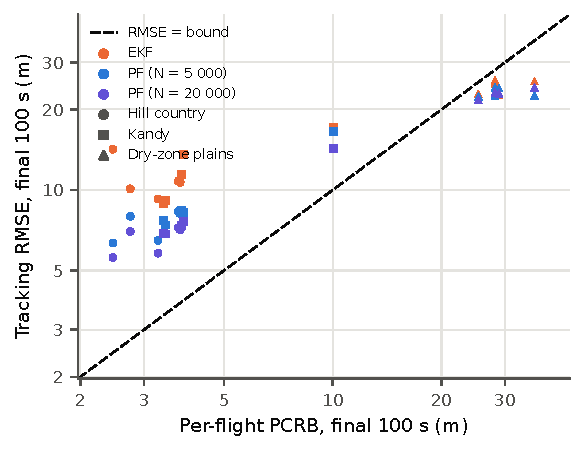
\includegraphics[width=0.6\textwidth]{e5_plans.pdf}
  \caption{E5: tracking RMSE of converged runs against the per-flight PCRB, for five fixed flight
    plans per region ($M = 100$ each, $\sigma_0 = 500$\,m). On the plains the bound is comparable
    to the 50\,m convergence threshold, so restricting the RMSE to converged runs truncates it
    and points fall below the diagonal; the unconditional RMSE never does.}\label{fig:e5plans}
\end{figure}

\paragraph{Why the filters stay above the bound.} Per flight (\cref{fig:e5plans,tab:e5plans}),
the converged 20\,000-particle PF tracks at \EFivePlanHillPfTwoZeroZeroZeroZeroRatio{} times the
bound on the hill country and \EFivePlanKandyPfTwoZeroZeroZeroZeroRatio{} times around Kandy
(medians over the five plans). This gap was tested rather than assumed: a Kalman filter that knows
the true terrain slopes along the path but uses the particle filter's tuning ($\sigma_p = 2$\,m per
step instead of the true $\approx 0.05$\,m) has an actual tracking RMSE of
\EFivePlanHillPfTwoZeroZeroZeroZeroTuned\,m on the hill country --- the mismatched-gain
recursion of \cref{app:mismatch} --- and the particle filter reaches
\EFivePlanHillPfTwoZeroZeroZeroZeroRmse\,m, i.e.\ \EFivePlanHillPfTwoZeroZeroZeroZeroRatioTuned{}
times what its tuning allows (Kandy: \EFivePlanKandyPfTwoZeroZeroZeroZeroRatioTuned). Nearly the
whole factor of two to the bound is the deliberate process-noise inflation, not the particle
approximation. With 5\,000 particles about 20\,\% of Monte Carlo error is added
(\EFivePlanHillPfFiveZeroZeroZeroRatioTuned); the EKF's converged runs are
\EFivePlanHillEkfRatioTuned{} times the tuned limit, because it linearises at its own estimate
rather than at the truth.

\subsection{E6 --- Detecting and recovering from false lock}\label{sec:e6}
\emph{Setup:} the divergence monitor of \cref{sec:monitor} (re-spread fraction $\alpha = 0.5$)
was tuned on separate development seeds ($M = \ESixDevRuns$ per cell; \cref{tab:e6dev}) with a
rule fixed in advance: the best convergence at $\sigma_0 = 2$\,km among settings with at most
5\,\% of runs raising an alarm at $\sigma_0 = 250$\,m. No setting met that constraint (the lowest
was 8\,\%), so --- decided on the development data before the test runs, and recorded as such ---
the setting with the fewest false alarms was taken: window $L = \ESixWindow$, $p_{\mathrm{FA}} =
\ESixPfa$. The test on the main seeds ($M = \ESixTestRuns$) compares, on identical flights, the
plain PF ($N = 5\,000$), the PF with the monitor, the PF with roughening ($K = 0.05$, the value
that worked best in E3) and the PF with both. The monitor against the plain PF is the primary
comparison; the other two were added because E3 had shown roughening to attack the same failure.

\begin{figure}[t]
  \centering
  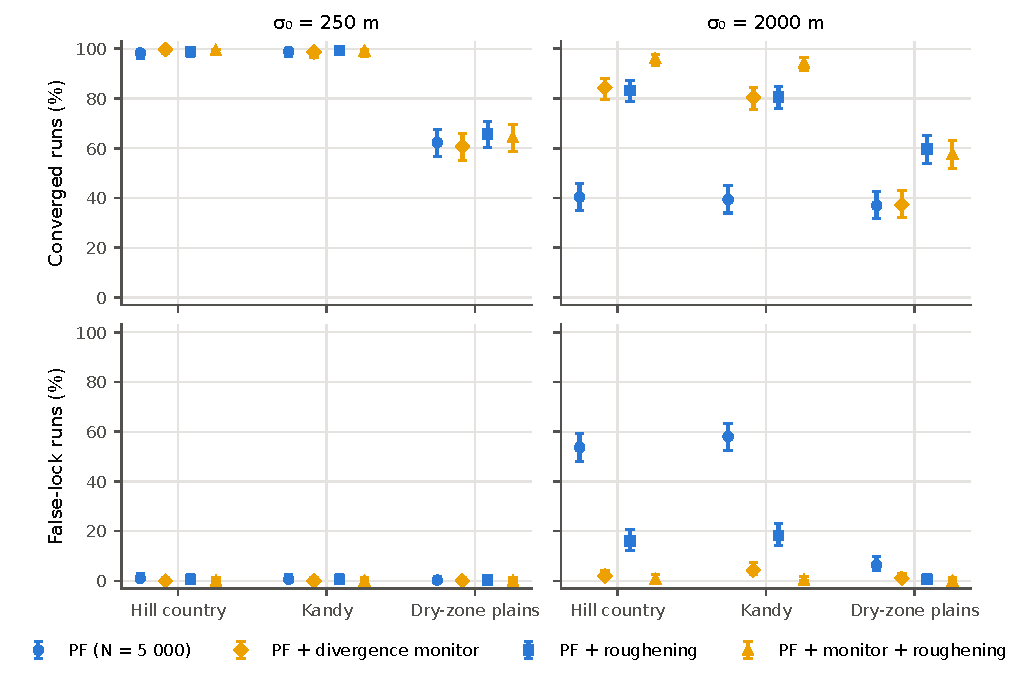
\includegraphics[width=\textwidth]{e6_test.pdf}
  \caption{E6: converged (top) and falsely locked (bottom) runs for the four variants at
    $\sigma_0 = 250$\,m and 2\,km, $M = \ESixTestRuns$ on the main seeds, Wilson 95\,\% intervals.}
  \label{fig:e6}
\end{figure}

The monitor does what it was designed for (\cref{fig:e6,tab:e6}). At $\sigma_0 = 2$\,km on the
hill country it raises convergence from \ESixHillSTwoZeroZeroZeroPfFiveZeroZeroZeroConv\,\% to
\ESixHillSTwoZeroZeroZeroPfMonitorConv\,\% and cuts false lock from
\ESixHillSTwoZeroZeroZeroPfFiveZeroZeroZeroFl\,\% to \ESixHillSTwoZeroZeroZeroPfMonitorFl\,\%
(Kandy: \ESixKandySTwoZeroZeroZeroPfFiveZeroZeroZeroConv\,\% $\to$
\ESixKandySTwoZeroZeroZeroPfMonitorConv\,\%; McNemar $p < 0.001$ on both regions). At
$\sigma_0 = 250$\,m, where it should stay silent, \ESixHillSTwoFiveZeroPfMonitorAlarm\,\% of the
hill-country runs raise an alarm, but convergence is unaffected
(\ESixHillSTwoFiveZeroPfFiveZeroZeroZeroConv\,\% $\to$ \ESixHillSTwoFiveZeroPfMonitorConv\,\%):
keeping half of the cloud means a false alarm costs little. On the plains the monitor changes
nothing (\ESixPlainsSTwoZeroZeroZeroPfFiveZeroZeroZeroConv\,\% vs.\
\ESixPlainsSTwoZeroZeroZeroPfMonitorConv\,\%), as expected: there the filter does not fail by locking
falsely, so there is nothing to detect.

Roughening alone is almost as effective on the hills
(\ESixHillSTwoZeroZeroZeroPfRoughConv\,\%) but leaves more false locks
(\ESixHillSTwoZeroZeroZeroPfRoughFl\,\%), and it is the only variant that helps on the plains
(\ESixPlainsSTwoZeroZeroZeroPfRoughConv\,\%). The two mechanisms are complementary: roughening
prevents locks by keeping hypotheses near the truth alive during acquisition; the monitor recovers
from those that still happen. Together they reach \ESixHillSTwoZeroZeroZeroPfMonitorRoughConv\,\%
(hill country) and \ESixKandySTwoZeroZeroZeroPfMonitorRoughConv\,\% (Kandy) at $\sigma_0 = 2$\,km,
with at most \ESixHillSTwoZeroZeroZeroPfMonitorRoughFl\,\% false locks --- better than the plain
filter with 20\,000 particles in E1 (\EOneHillSTwoZeroZeroZeroPfTwoZeroZeroZeroZeroConv\,\%), at a
quarter of the cost. With roughening, the monitor fires in only
\ESixHillSTwoZeroZeroZeroPfMonitorRoughAlarm\,\% of the hill-country runs instead of
\ESixHillSTwoZeroZeroZeroPfMonitorAlarm\,\%: there are fewer locks to catch.

\subsection{E7 --- Rao-Blackwellisation}\label{sec:e7}
\emph{Setup:} plain PF and RBPF with $N \in \{500, 1\,000, 2\,000, 5\,000\}$ on identical flights,
$\sigma_0 = 1$\,km, $M = \ESevenRuns$ per cell. The two filters cost the same per step at equal
$N$ (\cref{tab:runtime}), so equal $N$ is also equal runtime (\cref{fig:e7rt}).

\begin{figure}[t]
  \centering
  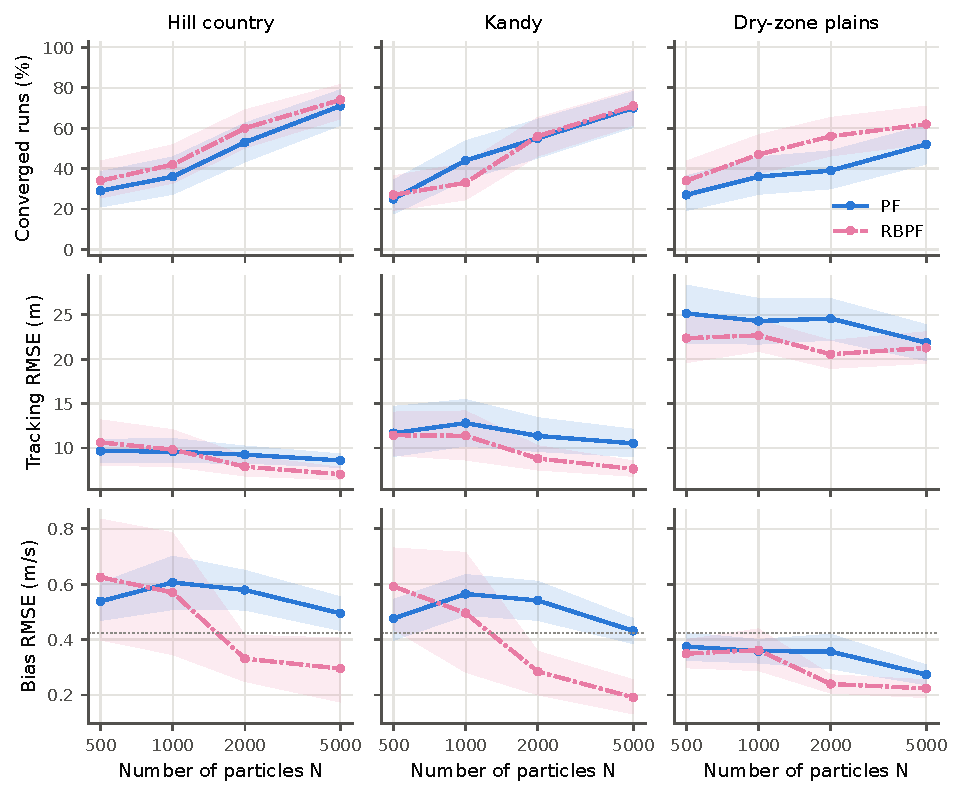
\includegraphics[width=\textwidth]{e7_equal_n.pdf}
  \caption{E7: plain PF vs.\ RBPF at equal particle count: convergence (top), tracking RMSE
    (middle) and RMS error of the INS-bias estimate in the tracking window (bottom; the prior
    alone gives 0.42\,m/s). $M = \ESevenRuns$, $\sigma_0 = 1$\,km, 95\,\% intervals.}\label{fig:e7}
\end{figure}

On the hilly regions the RBPF converges about as often as the plain PF (no significant difference,
McNemar $p \ge 0.09$; \cref{tab:e7}); on the plains it converges more often at every $N$
(\ESevenPlainsRbpfNTwoZeroZeroZeroConv\,\% vs.\ \ESevenPlainsPfNTwoZeroZeroZeroConv\,\% at
$N = 2\,000$, $p = 0.008$). Its clearest advantage is in the quantity it computes exactly
(\cref{fig:e7}): with $N = 5\,000$ on the hill country its bias estimate has an RMS error of
\ESevenHillRbpfNFiveZeroZeroZeroBias\,m/s, against \ESevenHillPfNFiveZeroZeroZeroBias\,m/s for the
plain PF --- whose bias estimate is \emph{no better than the prior} (0.42\,m/s). This is the
well-known impoverishment of an almost static parameter: the bias changes by only 0.002\,m/s
per step, so after repeated resampling all particles' bias values descend from a few ancestors,
and the estimate is roughly one random draw from the prior. The RBPF never samples the bias and
cannot impoverish it. The better bias carries over to tracking: from $N = 2\,000$ the RBPF's
tracking RMSE is lower (\ESevenHillRbpfNFiveZeroZeroZeroTrack{} vs.\
\ESevenHillPfNFiveZeroZeroZeroTrack\,m on the hill country at $N = 5\,000$). With 500 particles
the advantage disappears: each particle's bias filter is then driven by few, noisy position
increments.

\begin{figure}[t]
  \centering
  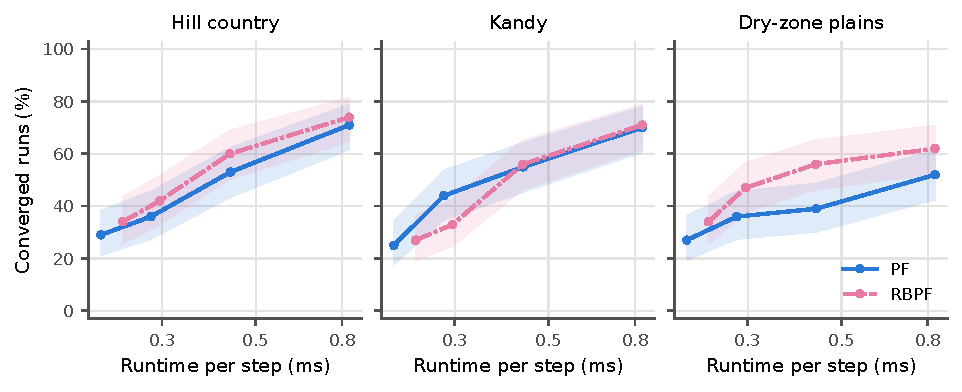
\includegraphics[width=\textwidth]{e7_equal_runtime.pdf}
  \caption{E7: convergence against runtime per step (single-core benchmark); $M = \ESevenRuns$.}
  \label{fig:e7rt}
\end{figure}

\subsection{Illustration}\label{sec:illustration}
\Cref{fig:snapshots,fig:trajectory} show one run, chosen by a fixed rule rather than by eye: the
lowest-index E1 run on the hill country with $\sigma_0 = 2$\,km in which the 20\,000-particle PF
converged after at least 60\,s and the EKF did not. It was re-simulated from its seeds with the
particle cloud recorded, reproducing the saved run exactly. Five seconds after take-off the cloud
has fragmented into clusters along terrain contours --- the multimodal posterior the EKF cannot
represent. By 20\,s it has collapsed onto one tight cluster some 100--150\,m from the truth, a
temporarily wrong mode, and between 60 and 150\,s the measurements move it onto the truth, where
it stays. Meanwhile the EKF confidently follows the wrong slope away from the truth and ends
further off than dead reckoning. An animation of this run (\texttt{report/figures/visuals\_animation.mp4})
is in the repository.

\begin{figure}[t]
  \centering
  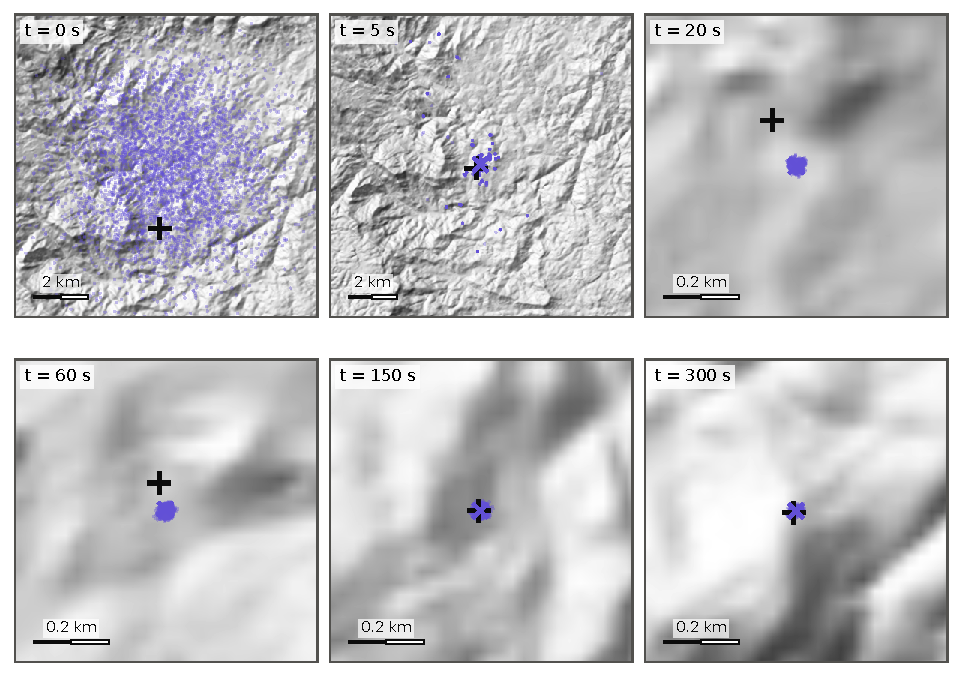
\includegraphics[width=\textwidth]{visuals_snapshots.pdf}
  \caption{Particle cloud (blue, 4\,000 of 20\,000 particles shown) over the hill-country
    hillshade at six instants of the illustrative run; $+$ truth, $\times$ PF estimate. Note the
    changing scale bars.}\label{fig:snapshots}
\end{figure}

\begin{figure}[t]
  \centering
  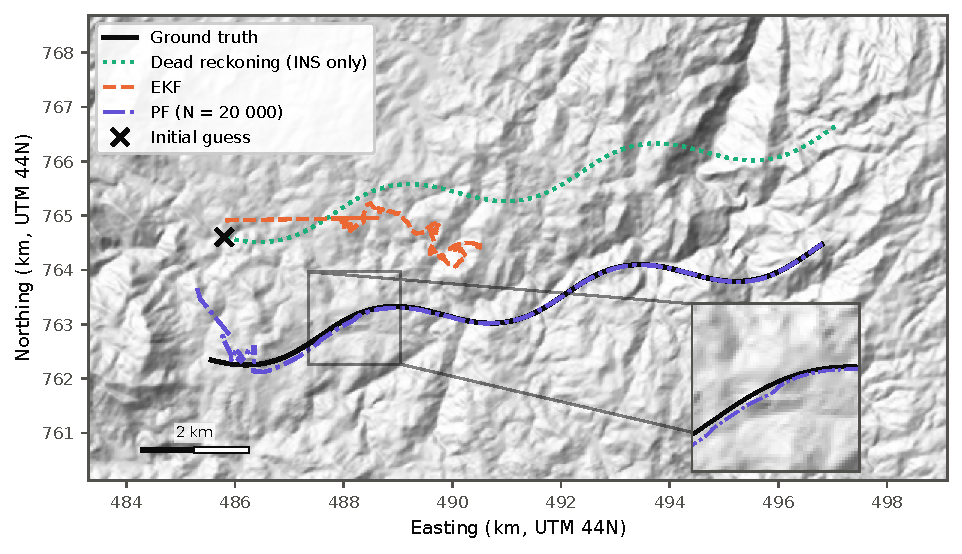
\includegraphics[width=\textwidth]{visuals_trajectory.pdf}
  \caption{Trajectories of the illustrative run; inset: the lock-on of the particle filter
    (20\,s before to 20\,s after its convergence time).}\label{fig:trajectory}
\end{figure}

\section{Discussion}\label{sec:discussion}

\subsection{Why the particle filter wins, and where the EKF breaks}
The decisive quantity is the ratio between the position uncertainty and the distance over which
the terrain slope stays roughly constant. The EKF replaces the terrain by its tangent plane at the
current estimate; that is adequate only when the error is small compared with the terrain's
correlation length. The smooth synthetic hills used during development have correlation lengths of
hundreds of metres to kilometres, and there the EKF held up to $\sigma_0 = 1$\,km. The real 30\,m
DEM of the hill country changes slope within a few cells, so the EKF already fails in
\EOneHillSOneZeroZeroEkfFl\,\% of the runs at $\sigma_0 = 100$\,m (E1). E2 shows the same effect
from the other side: the rougher the terrain under a flight, the \emph{larger} the EKF's error
($\rho = +\ETwoRhoEkf$) and the smaller the particle filter's ($\rho = \ETwoRhoPfFiveZeroZeroZero$).
Terrain texture is information for an estimator that evaluates the likelihood globally and noise
for one that linearises it locally.

Two consequences are worth stressing. First, a failed EKF is not merely inaccurate: its error
grows faster than that of the uncorrected INS, because corrections computed from the wrong slope
also corrupt its bias estimate (\cref{fig:e1time}). A linearised TAN filter whose linearisation is
invalid is worse than no terrain aiding. Second, its failures are confident: the EKF's dominant
failure mode is false lock (\cref{fig:e1rates}), so its own covariance gives no warning.

The particle filter pays for its robustness in computation, but on this problem the cost is
irrelevant: \RtPfFiveZeroZeroZero\,ms per step for 5\,000 particles on one laptop core, three
orders of magnitude inside the 1\,Hz measurement interval (E3).

\subsection{Terrain decides}
The three regions differ by two orders of magnitude in the information one altimeter sample
carries (\cref{tab:terrain}), and that ordering carries through every experiment. Over the hills
the particle filter tracks at 6--10\,m; over the plains at about 20--25\,m, close to the posterior
bound there (E5). The plains also show the most desirable property of a Bayesian filter: when the
terrain says little, the particle filter's covariance stays wide and it almost never locks
falsely (E1), so a navigation system could trust its own uncertainty and fall back on other
sources. The EKF has no such honesty --- it false-locks most often precisely where the terrain is
least informative relative to its linearisation errors.

The along-/cross-track decomposition (E2) did not show the elongated error along ridges and valleys
one might expect: averaged over flights with a 25$^\circ$ heading weave over 40\,km of varied
terrain, both directions are about equally constrained. The effect may exist on individual straight
flights along a valley, which this design does not isolate.

\subsection{Failure modes and their remedies}
\paragraph{False lock.} With a wide prior the particle filter's dominant failure is to collapse onto
the wrong patch of terrain (E1, E3). Three remedies were tested on identical flights: more particles
(E3: \EThreeNFiveKConv\,\% $\to$ \EThreeNTwentyKConv\,\% convergence from 5\,000 to 20\,000 at
$\sigma_0 = 1$\,km), roughening (E3: \EThreeRoughZeroPointZeroFiveConv\,\% with $K = 0.05$ at the
cost of 5\,000 particles) and the divergence monitor (E6). Roughening acts early, by keeping
hypotheses near the truth alive while the cloud is wide; the monitor acts late, by detecting a lock
that has already happened and re-opening the search.
On the main seeds (E6) the monitor alone lifts convergence at $\sigma_0 = 2$\,km on the hill
country from \ESixHillSTwoZeroZeroZeroPfFiveZeroZeroZeroConv\,\% to
\ESixHillSTwoZeroZeroZeroPfMonitorConv\,\%, roughening alone to
\ESixHillSTwoZeroZeroZeroPfRoughConv\,\%, and the two together to
\ESixHillSTwoZeroZeroZeroPfMonitorRoughConv\,\% with almost no false locks --- more than four
times as many particles achieve without them. The monitor's value lies in a property no amount of
particles provides: it turns a silent failure into a detected one, from information available on
board (the predicted innovation), without ground truth. Its false alarms are cheap because the
re-spread keeps half of the current cloud. Where the filter fails by imprecision rather than by
locking (the plains), there is nothing for the monitor to detect, and only roughening helps.

\paragraph{Altimeter outliers.} A Gaussian likelihood lets a single gross radar error destroy the
particles at the truth. The Student-$t$ likelihood keeps convergence at
\EFourOutliersHillOneZeroPfStudentTConv\,\% with 10\,\% outliers (Gaussian:
\EFourOutliersHillOneZeroPfFiveZeroZeroZeroConv\,\%) and costs nothing without them (E4). There is
no reason not to use it.

\paragraph{Map and altimeter offsets.} A random map error of the size the Copernicus handbook
implies is harmless, but a constant offset between measured and mapped height --- a barometric
bias, or a radar seeing through a canopy the surface model includes --- defeats the filter beyond
about 5\,m (E4). Inflating $\sigma_z$ buys tolerance up to about 10\,m; estimating the offset as a
state is the only remedy at 20\,m but costs acquisition when there is no offset. The obvious next
step is to treat the offset like the bias in the RBPF: it enters the measurement linearly, so it
could be marginalised analytically instead of sampled.

\paragraph{Static-parameter impoverishment.} The plain particle filter cannot estimate the INS bias
(E7): with a nearly static bias, resampling leaves bias values from a few ancestors, and the
estimate is no better than the prior. Rao-Blackwellisation removes the problem at no extra cost and
improves tracking from 2\,000 particles. It is the better filter for this model.

\subsection{How close to optimal?}
The posterior Cramér--Rao bound is never violated, which checks the whole chain of simulation,
filters and bound. In the tracking phase the filters are about twice the per-flight bound on the
hills, and the mismatched-gain analysis shows why: the deliberately inflated process noise
($\sigma_p = 2$\,m per step vs.\ a true $\approx0.05$\,m) alone allows only
\EFivePlanHillPfTwoZeroZeroZeroZeroTuned\,m, and the 20\,000-particle PF reaches
\EFivePlanHillPfTwoZeroZeroZeroZeroRmse\,m (E5). The inflation is a deliberate trade:
smaller process noise would track closer to the bound but would make the cloud less diverse during
acquisition, where E3 shows diversity (roughening) to be what matters. During acquisition the
bound is not a useful benchmark, because it ignores ambiguity --- which is precisely what makes TAN
hard; a bound that accounts for ambiguity would be needed there. The NEES behaves accordingly: consistent to conservative in the tracking phase,
uninformative while the posterior is multimodal.

\subsection{Limitations}\label{sec:limitations}
\begin{itemize}
  \item \textbf{Simulated sensors and flights.} No real flight data were used. The altimeter noise
        (2\,m barometric, 3\,m radar, white and range-independent) is an assumption, and an
        optimistic one at the 1--1.7\,km radar ranges the corridor altitude produces over the
        hills (E1).
  \item \textbf{Simplified flight.} Constant altitude and a horizontal 2-D state; attitude, height
        and their errors are not estimated, and the INS model is a velocity bias plus white noise.
  \item \textbf{The world uses the same map.} The simulated radar sees the DEM itself unless E4
        adds a map error; real canopy and DSM effects are spatially structured and only
        approximated by a smooth random field and a constant offset.
  \item \textbf{One tuning.} Process and measurement noise were fixed, not optimised per filter;
        the EKF in particular might do somewhat better with different tuning, although its failures
        are structural (linearisation), not a matter of noise levels.
  \item \textbf{Three regions of one country.} The conclusions about terrain dependence rest on
        three 40\,km boxes; they are consistent with the per-flight analysis of E2, but other
        landscapes (urban, forest, desert dunes) were not tested.
\end{itemize}

\subsection{Future work}
Natural extensions are a Rao-Blackwellised offset state, an adaptive proposal that uses the
current measurement (auxiliary or likelihood-based proposals) to fight false lock at its source,
a point-mass filter as a deterministic reference, real flight data with a recorded radar
altimeter, and an ambiguity-aware performance bound for the acquisition phase.

\section{Conclusion}\label{sec:conclusion}

A particle filter for terrain-aided navigation was implemented, validated against the exact
Kalman filter on planar terrain, and evaluated over real terrain of Sri Lanka in seven Monte Carlo
experiments. The main conclusions are:

\begin{enumerate}
  \item \textbf{The particle filter is the right tool, and real terrain makes the case more
        strongly than synthetic terrain.} Over real hills the EKF already locks falsely in
        \EOneHillSOneZeroZeroEkfFl\,\% of runs at 100\,m initial error and converges in only
        \EOneHillSFiveZeroZeroEkfConv\,\% at 500\,m (synthetic hills:
        \EOneSynthSFiveZeroZeroEkfConv\,\%); this ungated EKF then ends worse than dead reckoning.
        With 20\,000 particles the particle filter still converges in
        \EOneHillSOneZeroZeroZeroPfTwoZeroZeroZeroZeroConv\,\% of the runs at 1\,km and tracks at
        \EOneHillSFiveZeroZeroPfTwoZeroZeroZeroZeroTrack--\EOneKandySFiveZeroZeroPfTwoZeroZeroZeroZeroTrack\,m
        over the hills.
  \item \textbf{Terrain decides what is possible.} Performance follows the terrain information,
        strongly between terrain types and weakly between flights over the same hilly region; over
        flat plains the particle filter stays honestly uncertain instead of locking falsely.
  \item \textbf{False lock is the failure to design against.} More particles help, but roughening
        and a divergence monitor that needs no ground truth are complementary and reach
        \ESixHillSTwoZeroZeroZeroPfMonitorRoughConv\,\% convergence at 2\,km initial uncertainty
        with 5\,000 particles. The resampling scheme and the ESS threshold, by contrast, made no
        significant difference.
  \item \textbf{Robustness and efficiency.} A Student-$t$ likelihood removes most of the
        sensitivity to (zero-mean, 100\,m) altimeter outliers at no cost; constant map or altimeter
        offsets of 10\,m and more remain the most damaging model error; Rao-Blackwellising the INS
        bias fixes the plain filter's impoverished bias estimate once the position is locked on,
        at no extra runtime.
  \item \textbf{How far from optimal.} The unconditional error never undercuts the ensemble
        posterior Cramér--Rao bound; in the tracking phase the 20\,000-particle filter stays about
        twice above the per-flight bound, almost entirely because of its deliberately inflated
        process noise --- a trade made for robust acquisition, where the bound, blind to ambiguity,
        is not informative.
\end{enumerate}

Every number, table and figure in this report is regenerated from saved results by scripts in the
repository, and the study regions and analysis rules were fixed before the experiments ran.


\bibliographystyle{unsrtnat}
\bibliography{references}

\appendix
\section{Parameters}\label{app:params}

\begin{table}[H]
  \centering\small
  \caption{Simulation, sensor, filter and evaluation parameters (defaults; experiments that
    change one say so). Generated from \texttt{configs/default.yaml} and
    \texttt{configs/experiments/\_common.yaml}.}\label{tab:params}
  % Generated by scripts — do not edit.
\begin{tabular}{lllr}
\toprule
Group & Parameter & Value & Unit \\
\midrule
Simulation & Time step $\Delta t$ & 1 & s \\
Simulation & Flight duration & 300 & s \\
Simulation & Ground speed & 40 & m/s \\
Simulation & Heading weave amplitude & 25 & deg \\
Simulation & Heading weave period & 120 & s \\
Simulation & Clearance above highest terrain in corridor & 300 & m \\
Simulation & Corridor half-width & 1000 & m \\
Simulation & Flight margin from map edge / 3 & 2000 & m \\
Sensors & INS initial bias std (per axis) & 0.3 & m/s \\
Sensors & INS bias random walk & 0.002 & m/s/$\sqrt{\mathrm{s}}$ \\
Sensors & INS white velocity noise & 0.05 & m/s \\
Sensors & Barometric altimeter noise & 2 & m \\
Sensors & Radar altimeter noise & 3 & m \\
Sensors & Radar outlier std (E4) & 100 & m \\
Prior & Initial position std $\sigma_0$ (default) & 500 & m \\
Particle filter & Particles $N$ (default) & 5000 &  \\
Particle filter & Resampling scheme & systematic &  \\
Particle filter & Resample when $N_\mathrm{eff} < \tau N$, $\tau$ & 0.5 &  \\
Particle filter & Process noise, position $\sigma_p$ & 2 & m/step \\
Particle filter & Process noise, bias $\sigma_b$ & 0.002 & m/s/step \\
Particle filter & Measurement std $\sigma_z$ & 3.6 & m \\
Particle filter & Roughening $K$ (default) & 0 &  \\
Evaluation & Convergence threshold & 50 & m \\
Evaluation & Tracking window & 100 & s \\
\bottomrule
\end{tabular}

\end{table}

\section{Reproducibility}\label{app:repro}

\paragraph{Machine.} All runtimes refer to one laptop: \MachineCpu{} (6 performance and 4
efficiency cores), 16\,GB RAM, \MachineOs{}, Python \MachinePython{}, NumPy \MachineNumpy{}.

\paragraph{Reproducing everything.} From a fresh clone with an OpenTopography API key in
\texttt{.env}:
\begin{lstlisting}[language=bash,numbers=none]
make setup        # virtual environment + package + test tools
make test         # unit tests
make data         # download, reproject and crop the three regions (4 API calls)
make benchmark    # runtime per filter step (run on an idle machine)
make experiments  # all Monte Carlo experiments (resumable; about an hour on this laptop)
make figures      # every figure, table and number in this report, from saved results
make report       # this PDF (or upload report/ to Overleaf)
\end{lstlisting}
\texttt{make quick} runs every experiment with three runs and short flights as a smoke test, and
\texttt{make smoke} checks the whole pipeline on synthetic terrain without any download.
Each results folder stores the git commit, the data-manifest checksum, the resolved configuration
of every experiment cell and the installed package versions; \texttt{data/manifest.json} stores
SHA-256 checksums of every raster.

\paragraph{Code.} Repository: \texttt{https://github.com/KaveeshwaraBandara/terrain-aided-navigation-pf}.

\paragraph{Data attribution.} Produced using Copernicus WorldDEM-30 \textcopyright{} DLR e.V.
2010--2014 and \textcopyright{} Airbus Defence and Space GmbH 2014--2018 provided under
COPERNICUS by the European Union and ESA; all rights reserved. Data accessed through
OpenTopography.


\end{document}
